% Options for packages loaded elsewhere
\PassOptionsToPackage{unicode}{hyperref}
\PassOptionsToPackage{hyphens}{url}
\PassOptionsToPackage{dvipsnames,svgnames*,x11names*}{xcolor}
%
\documentclass[
  11pt,
]{krantz}
\usepackage{lmodern}
\usepackage{amssymb,amsmath}
\usepackage{ifxetex,ifluatex}
\ifnum 0\ifxetex 1\fi\ifluatex 1\fi=0 % if pdftex
  \usepackage[T1]{fontenc}
  \usepackage[utf8]{inputenc}
  \usepackage{textcomp} % provide euro and other symbols
\else % if luatex or xetex
  \usepackage{unicode-math}
  \defaultfontfeatures{Scale=MatchLowercase}
  \defaultfontfeatures[\rmfamily]{Ligatures=TeX,Scale=1}
\fi
% Use upquote if available, for straight quotes in verbatim environments
\IfFileExists{upquote.sty}{\usepackage{upquote}}{}
\IfFileExists{microtype.sty}{% use microtype if available
  \usepackage[]{microtype}
  \UseMicrotypeSet[protrusion]{basicmath} % disable protrusion for tt fonts
}{}
\makeatletter
\@ifundefined{KOMAClassName}{% if non-KOMA class
  \IfFileExists{parskip.sty}{%
    \usepackage{parskip}
  }{% else
    \setlength{\parindent}{0pt}
    \setlength{\parskip}{6pt plus 2pt minus 1pt}}
}{% if KOMA class
  \KOMAoptions{parskip=half}}
\makeatother
\usepackage{xcolor}
\IfFileExists{xurl.sty}{\usepackage{xurl}}{} % add URL line breaks if available
\IfFileExists{bookmark.sty}{\usepackage{bookmark}}{\usepackage{hyperref}}
\hypersetup{
  pdftitle={통계 프로그래밍 언어},
  pdfauthor={한국한의학연구원, 구본초},
  colorlinks=true,
  linkcolor=Maroon,
  filecolor=Maroon,
  citecolor=Blue,
  urlcolor=Blue,
  pdfcreator={LaTeX via pandoc}}
\urlstyle{same} % disable monospaced font for URLs
\usepackage{color}
\usepackage{fancyvrb}
\newcommand{\VerbBar}{|}
\newcommand{\VERB}{\Verb[commandchars=\\\{\}]}
\DefineVerbatimEnvironment{Highlighting}{Verbatim}{commandchars=\\\{\}}
% Add ',fontsize=\small' for more characters per line
\usepackage{framed}
\definecolor{shadecolor}{RGB}{248,248,248}
\newenvironment{Shaded}{\begin{snugshade}}{\end{snugshade}}
\newcommand{\AlertTok}[1]{\textcolor[rgb]{0.33,0.33,0.33}{#1}}
\newcommand{\AnnotationTok}[1]{\textcolor[rgb]{0.37,0.37,0.37}{\textbf{\textit{#1}}}}
\newcommand{\AttributeTok}[1]{\textcolor[rgb]{0.61,0.61,0.61}{#1}}
\newcommand{\BaseNTok}[1]{\textcolor[rgb]{0.06,0.06,0.06}{#1}}
\newcommand{\BuiltInTok}[1]{#1}
\newcommand{\CharTok}[1]{\textcolor[rgb]{0.5,0.5,0.5}{#1}}
\newcommand{\CommentTok}[1]{\textcolor[rgb]{0.37,0.37,0.37}{\textit{#1}}}
\newcommand{\CommentVarTok}[1]{\textcolor[rgb]{0.37,0.37,0.37}{\textbf{\textit{#1}}}}
\newcommand{\ConstantTok}[1]{\textcolor[rgb]{0,0,0}{#1}}
\newcommand{\ControlFlowTok}[1]{\textcolor[rgb]{0.27,0.27,0.27}{\textbf{#1}}}
\newcommand{\DataTypeTok}[1]{\textcolor[rgb]{0.27,0.27,0.27}{#1}}
\newcommand{\DecValTok}[1]{\textcolor[rgb]{0.06,0.06,0.06}{#1}}
\newcommand{\DocumentationTok}[1]{\textcolor[rgb]{0.37,0.37,0.37}{\textbf{\textit{#1}}}}
\newcommand{\ErrorTok}[1]{\textcolor[rgb]{0.14,0.14,0.14}{\textbf{#1}}}
\newcommand{\ExtensionTok}[1]{#1}
\newcommand{\FloatTok}[1]{\textcolor[rgb]{0.06,0.06,0.06}{#1}}
\newcommand{\FunctionTok}[1]{\textcolor[rgb]{0,0,0}{#1}}
\newcommand{\ImportTok}[1]{#1}
\newcommand{\InformationTok}[1]{\textcolor[rgb]{0.37,0.37,0.37}{\textbf{\textit{#1}}}}
\newcommand{\KeywordTok}[1]{\textcolor[rgb]{0.27,0.27,0.27}{\textbf{#1}}}
\newcommand{\NormalTok}[1]{#1}
\newcommand{\OperatorTok}[1]{\textcolor[rgb]{0.43,0.43,0.43}{\textbf{#1}}}
\newcommand{\OtherTok}[1]{\textcolor[rgb]{0.37,0.37,0.37}{#1}}
\newcommand{\PreprocessorTok}[1]{\textcolor[rgb]{0.37,0.37,0.37}{\textit{#1}}}
\newcommand{\RegionMarkerTok}[1]{#1}
\newcommand{\SpecialCharTok}[1]{\textcolor[rgb]{0,0,0}{#1}}
\newcommand{\SpecialStringTok}[1]{\textcolor[rgb]{0.5,0.5,0.5}{#1}}
\newcommand{\StringTok}[1]{\textcolor[rgb]{0.5,0.5,0.5}{#1}}
\newcommand{\VariableTok}[1]{\textcolor[rgb]{0,0,0}{#1}}
\newcommand{\VerbatimStringTok}[1]{\textcolor[rgb]{0.5,0.5,0.5}{#1}}
\newcommand{\WarningTok}[1]{\textcolor[rgb]{0.37,0.37,0.37}{\textbf{\textit{#1}}}}
\usepackage{longtable,booktabs}
% Correct order of tables after \paragraph or \subparagraph
\usepackage{etoolbox}
\makeatletter
\patchcmd\longtable{\par}{\if@noskipsec\mbox{}\fi\par}{}{}
\makeatother
% Allow footnotes in longtable head/foot
\IfFileExists{footnotehyper.sty}{\usepackage{footnotehyper}}{\usepackage{footnote}}
\makesavenoteenv{longtable}
\usepackage{graphicx,grffile}
\makeatletter
\def\maxwidth{\ifdim\Gin@nat@width>\linewidth\linewidth\else\Gin@nat@width\fi}
\def\maxheight{\ifdim\Gin@nat@height>\textheight\textheight\else\Gin@nat@height\fi}
\makeatother
% Scale images if necessary, so that they will not overflow the page
% margins by default, and it is still possible to overwrite the defaults
% using explicit options in \includegraphics[width, height, ...]{}
\setkeys{Gin}{width=\maxwidth,height=\maxheight,keepaspectratio}
% Set default figure placement to htbp
\makeatletter
\def\fps@figure{htbp}
\makeatother
\setlength{\emergencystretch}{3em} % prevent overfull lines
\providecommand{\tightlist}{%
  \setlength{\itemsep}{0pt}\setlength{\parskip}{0pt}}
\setcounter{secnumdepth}{5}
\usepackage{kotex}
\usepackage{dhucs-cmap}
\usepackage{booktabs}
\usepackage{placeins}
\usepackage{enumerate}
\usepackage{amssymb}
\usepackage{amsmath}
\usepackage{mathtools}
\usepackage{float}
% \usepackage{setspace} \doublespacing
\usepackage{relsize}
\usepackage{bigints}
\usepackage{bm}
\usepackage{amsmath}
% \usepackage{titlesec}
\usepackage{lipsum}
\usepackage{longtable}
 \usepackage[font=small,labelfont=bf]{caption}
\usepackage{dcolumn}
\usepackage{array}
\usepackage{gensymb}
\usepackage{makecell}
\usepackage{multirow}
\usepackage{natbib}
\usepackage{rotating}
\usepackage[most]{tcolorbox}

\renewcommand\theadalign{cb}
\renewcommand\theadfont{\bfseries}
\renewcommand\theadgape{\Gape[4pt]}
\renewcommand\cellgape{\Gape[4pt]}
\DeclareMathAlphabet{\mathpzc}{OT1}{pzc}{m}{it}

\renewcommand\theadalign{cb}
\renewcommand\theadfont{\bfseries}
\renewcommand\theadgape{\Gape[4pt]}
\renewcommand\cellgape{\Gape[4pt]}

\newcolumntype{L}[1]{>{\raggedright\let\newline\\
\arraybackslash\hspace{0pt}}m{#1}}
\newcolumntype{C}[1]{>{\centering\let\newline\\
\arraybackslash\hspace{0pt}}m{#1}}
\newcolumntype{R}[1]{>{\raggedleft\let\newline\\
\arraybackslash\hspace{0pt}}m{#1}}
\newcolumntype{P}[1]{>{\raggedright\tabularxbackslash}p{#1}}
\newcommand{\specialcell}[2][c]{%
  \begin{tabular}[#1]{@{}c@{}}#2\end{tabular}}
\newcommand{\specialcelll}[2][l]{%
  \begin{tabular}[#1]{@{}l@{}}#2\end{tabular}}

\captionsetup[table]{aboveskip=0pt}
\captionsetup[table]{belowskip=10pt}

\linespread{1.5}

% \setmainfont[UprightFeatures={SmallCapsFont=AlegreyaSC-Regular}]{Alegreya}

\usepackage{framed,color}
\definecolor{shadecolor}{RGB}{248,248,248}

\renewcommand{\textfraction}{0.05}
\renewcommand{\topfraction}{0.8}
\renewcommand{\bottomfraction}{0.8}
\renewcommand{\floatpagefraction}{0.75}

% \renewenvironment{quote}{\begin{VF}}{\end{VF}}
\let\oldhref\href
\renewcommand{\href}[2]{#2\footnote{\url{#1}}}

\ifxetex
  \usepackage{letltxmacro}
  \setlength{\XeTeXLinkMargin}{1pt}
  \LetLtxMacro\SavedIncludeGraphics\includegraphics
  \def\includegraphics#1#{% #1 catches optional stuff (star/opt. arg.)
    \IncludeGraphicsAux{#1}%
  }%
  \newcommand*{\IncludeGraphicsAux}[2]{%
    \XeTeXLinkBox{%
      \SavedIncludeGraphics#1{#2}%
    }%
  }%
\fi

\makeatletter
\newenvironment{kframe}{%
\medskip{}
\setlength{\fboxsep}{.8em}
 \def\at@end@of@kframe{}%
 \ifinner\ifhmode%
  \def\at@end@of@kframe{\end{minipage}}%
  \begin{minipage}{\columnwidth}%
 \fi\fi%
 \def\FrameCommand##1{\hskip\@totalleftmargin \hskip-\fboxsep
 \colorbox{shadecolor}{##1}\hskip-\fboxsep
     % There is no \\@totalrightmargin, so:
     \hskip-\linewidth \hskip-\@totalleftmargin \hskip\columnwidth}%
 \MakeFramed {\advance\hsize-\width
   \@totalleftmargin\z@ \linewidth\hsize
   \@setminipage}}%
 {\par\unskip\endMakeFramed%
 \at@end@of@kframe}
\makeatother

\makeatletter
\@ifundefined{Shaded}{
}{\renewenvironment{Shaded}{\begin{kframe}}{\end{kframe}}}
\makeatother

\newenvironment{rmdblock}[1]
  {
  \begin{itemize}
  \renewcommand{\labelitemi}{
    \raisebox{-.7\height}[0pt][0pt]{
      {\setkeys{Gin}{width=3em,keepaspectratio}\includegraphics{images/#1}}
    }
  }
  \setlength{\fboxsep}{1em}
  \begin{kframe}
  \item
  }
  {
  \end{kframe}
  \end{itemize}
  }
  
\newenvironment{rmdnote}
  {\begin{rmdblock}{note}}
  {\end{rmdblock}}
  
\newenvironment{rmdcaution}
  {\begin{rmdblock}{caution}}
  {\end{rmdblock}}
  
\newenvironment{rmdimportant}
  {\begin{rmdblock}{important}}
  {\end{rmdblock}}
  
\newenvironment{rmdtip}
  {\begin{rmdblock}{tip}}
  {\end{rmdblock}}
  
\newenvironment{rmdwarning}
  {\begin{rmdblock}{warning}}
  {\end{rmdblock}}

\renewenvironment{quote}{\begin{kframe}}{\end{kframe}}

% \newenvironment{quoteshade}
%   {
%   \begin{itemize}
%   \begin{kframe}
%   \item
%   }
%   {
%   \end{kframe}
%   \end{itemize}
%   }
%   
% \newenvironment{rmdquote}
%  {\begin{quoteshade}}
%  {\end{quoteshade}}

\usepackage{makeidx}
\makeindex

\urlstyle{tt}

\usepackage{amsthm}
\makeatletter
\def\thm@space@setup{%
  \thm@preskip=8pt plus 2pt minus 4pt
  \thm@postskip=\thm@preskip
}
\makeatother

\frontmatter
\usepackage{booktabs}
\usepackage{longtable}
\usepackage{array}
\usepackage{multirow}
\usepackage{wrapfig}
\usepackage{float}
\usepackage{colortbl}
\usepackage{pdflscape}
\usepackage{tabu}
\usepackage{threeparttable}
\usepackage{threeparttablex}
\usepackage[normalem]{ulem}
\usepackage{makecell}
\usepackage{xcolor}
\usepackage[]{natbib}
\bibliographystyle{apalike}

\title{통계 프로그래밍 언어}
\usepackage{etoolbox}
\makeatletter
\providecommand{\subtitle}[1]{% add subtitle to \maketitle
  \apptocmd{\@title}{\par {\large #1 \par}}{}{}
}
\makeatother
\subtitle{2020년도 1학기 충남대학교 정보통계학과 강의 노트}
\author{한국한의학연구원, 구본초}
\date{2020-03-26}

\let\BeginKnitrBlock\begin \let\EndKnitrBlock\end
\begin{document}
\maketitle

{
\hypersetup{linkcolor=}
\setcounter{tocdepth}{2}
\tableofcontents
}
\listoftables
\listoffigures
\hypertarget{overview}{%
\chapter*{Course Overview}\label{overview}}


\BeginKnitrBlock{rmdnote}
본 문서는 2020년도 1학기 정보통계학과에서 개설한 ``통계 프로그래밍 언어'' 강의를 위해 개발한 강의 노트이고 주 단위로 업데이트될 예정임. 본 강의 노트는 \url{https://zorba78.github.io/cnu-r-programming-lecture-note/} 에서 확인할 수 있고, 해당 페이지에서 pdf 파일 다운로드가 가능함. 본 문서는 Yihui Xie가 개발한 \textbf{bookdown} 패키지 \citep{xie-2016}를 활용하여 생성한 문서이고 Google Chrome 또는 Firefox 브라우저에 최적화 됨. 아울러 충남대학교 정보통계학과 이상인 교수님의 2019년도 2학기 ``통계패키지활용'' 강의 노트와 동국대학교 ICT빅데이터학부 김진석 교수님의 \href{http://datamining.dongguk.ac.kr/lectures/R/_book/index.html}{R 프로그래밍 및 실습} 강의 자료 내용과 구성을 참고하여 작성함.

재택 수업 시 학생들이 사용하고 있는 컴퓨터의 인터넷 접속이 원활하다는 가정 하에서 강의를 진행할 예정이기 때문에 수강 시 온라인 상태 유지가 필수임.
\EndKnitrBlock{rmdnote}

\hypertarget{intro-lec}{%
\subsubsection*{강의소개}\label{intro-lec}}


R은 뉴질랜드 오클랜드 대학의 Robert Gentleman 과 Ross Ihaka 가 AT\&T 벨 연구소에서 개발한 S 언어를 기반으로 개발한 GNU 환경의 통계 계산 및 프로그래밍 언어이다. 현재 R 소프트웨어는 통계학 뿐 아니라 데이터 과학을 포함한 의학, 생물학 등 다양한 분야에서 활용되고 있으며 특히 통계 소프트웨어 개발과 데이터 분석에 많이 활용되고 있다. 본 강의는 데이터 분석을 위한 R의 기초 문법과 통계학 입문에서 학습한 몇 가지 중요한 통계적 이론에 대한 시뮬레이션 방법을 다룬다. 아울러 R package를 활용한 데이터 헨들링 및 시각화 그리고 Rmarkdown을 활용한 재현가능(reproducible)한 문서 작성법에 대해 학습하고자 한다.

\hypertarget{purpose-course}{%
\subsubsection*{교과 목표}\label{purpose-course}}


\begin{quote}
\begin{itemize}
\tightlist
\item
  \textbf{R 기초 문법 습득}
\item
  \textbf{R package를 활용한 데이터 핸들링 및 자료 시각화}
\item
  \textbf{R 시뮬레이션을 통한 통계학 기초 이론 확인}
\item
  \textbf{R을 이용한 데이터 분석 실습}
\item
  \textbf{R markdown을 이용한 재현가능(reproducible)한 보고서 작성 방법 습득}
\end{itemize}
\end{quote}

\hypertarget{pre-course}{%
\subsubsection*{선수과목}\label{pre-course}}


\begin{quote}
\textbf{통계학 개론}
\end{quote}

\hypertarget{course-method}
\item
  \textbf{실험/실습: 50\%}
\end{itemize}

\hypertarget{grade-method}
\item
  \textbf{기말고사: 40 \%}
\item
  \textbf{출석: 10 \%}
\item
  \textbf{과제: 10 \%}
\end{itemize}
\end{quote}

\hypertarget{policy-course}{%
\subsubsection*{수업 규정}\label{policy-course}}


\begin{quote}
\begin{itemize}
\tightlist
\item
  3번 지각은 1번 결석으로 처리
\item
  특별한 사유 없이 수업 중간에 이탈한 경우 결석으로 처리
\item
  특별한 사유로 인해 결석 또는 지각을 할 경우 사유를 증빙할 수 있는 서류 제출 시 출석으로 인정
\item
  출결 미달, 중간 또는 기말고사 미 응시인 경우 F 학점으로 처리
\item
  수업 중 휴대폰 및 각종 모바일 기기 사용 금지
\end{itemize}
\end{quote}

\hypertarget{material-course}{%
\subsubsection*{교재 및 참고문헌}\label{material-course}}


\begin{quote}
별도의 교재 없이 본 강의 노트로 수업을 진행할 예정이며, 수업의 이해도 향상을 위해 아래 소개할 도서 및 웹 문서 등을 참고할 것을 권장함.
\end{quote}

\textbf{참고 자료}

\begin{itemize}
\tightlist
\item
  빅데이터 분석 도구 R 프로그래밍 \citep{noman-2012}
\item
  실리콘밸리 데이터과학자가 알려주는 따라하며 배우는 데이터 과학 \citep{kwon-2017}
\item
  R을 이용한 데이터 처리\&분석 \citep{seo-2014}
\item
  R 그래픽스 \citep{ryu-2005}
\item
  \href{https://ggplot2-book.org/}{ggplot2: elegant graphics for data analysis} \citep{wickham-2016}
\item
  \href{https://r4ds.had.co.nz/}{R for data science} \citep{wickham-2016r}
\item
  Statistical Computing with R \citep{rizzo-2019}
\end{itemize}

\hypertarget{course-schedule}{%
\subsubsection*{강의 계획}\label{course-schedule}}


\begin{table}[H]

\caption{\label{tab:make-schedule-tab}강의 계획표}
\centering
\fontsize{10}{12}\selectfont
\begin{tabular}[t]{c>{\raggedright\arraybackslash}p{6cm}c}
\toprule
주차 & 강의 내용 & 과제\\
\midrule
\rowcolor{gray!6}  Week 1 & R 소개, R/R Studio 설치, R 패키지 설치, R 맛보기 및 markdown 문서 만들기 & 과제 1\\
Week 2 & R 자료형: 스칼라, 벡터, 리스트 & \\
\rowcolor{gray!6}  Week 3 & R 자료형: 행렬 및 배열 & 과제 2\\
Week 4 & R 자료형: 팩터, 테이블, 데이터 프레임 & \\
\rowcolor{gray!6}  Week 5 & R 자료형: 문자열과 정규 표현식 & 과제 3\\
\addlinespace
Week 6 & 데이터 프레임 가공 및 시각화 I & \\
\rowcolor{gray!6}  Week 7 & 데이터 프레임 가공 및 시각화 II & 과제 4\\
Week 8 & 중간고사 & \\
\rowcolor{gray!6}  Week 9 & 데이터 프레임 가공 및 시각화 III & \\
Week 10 & R 프로그래밍: 조건문, 반복문, 함수 & 과제 5\\
\addlinespace
\rowcolor{gray!6}  Week 11 & 통계시뮬레이션 I: 표본분포 및 중심극한정리 & \\
Week 12 & 통계시뮬레이션 2: 신뢰구간과 가설검정 & 과제 6\\
\rowcolor{gray!6}  Week 13 & R을 이용한 기초통계 분석 & \\
Week 14 & R markdown 활용 & 과제 7\\
\rowcolor{gray!6}  Week 15 & 기말고사 & \\
\bottomrule
\end{tabular}
\end{table}

\mainmatter

\hypertarget{part-get-started}{%
\part{Get Started}\label{part-get-started}}

\hypertarget{intro-chap}{%
\chapter{Introduction}\label{intro-chap}}

\textbf{1. R프로그램}

\begin{itemize}
\tightlist
\item
  데이터 분석을 위한 자료 전처리, 통계 및 시각화를 지원하는 컴퓨터 언어 및 환경
\item
  1980년 AT\&T 벨 연구소의 John Chambers가 개발한 S 언어를 기반으로 1995년 뉴질랜드 Auckland 대학의 통계학과 교수 Robert Gentleman과 Ross Ihaka 가 개발
\item
  \href{https://en.wikipedia.org/wiki/GNU_Project}{GNU} 기반의 오픈 소스
\item
  통계학, 전산학, 생물학, 의학 등 거의 모든 학문분야에서 분석도구로 활용되고 있고, 최근 data science 분야에서 널리 활용
\end{itemize}

\textbf{2. R 언어의 특징}

\begin{itemize}
\tightlist
\item
  \textbf{무료 소프트웨어}
\item
  \href{http://cran.r-project.org/web/view}{CRAN (Comprehensive R Archive Network)}에서 배포
\item
  특정 vendor가 아닌 전 세계 연구자들이 개발한 알고리즘 및 최신 함수 활용 가능(packaging system)
\item
  범용적으로 사용되는 거의 대부분의 운영체제(Windows, Mac, Linux)에서 작동 가능
\item
  방대한 개발 및 사용 생태계 형성
\item
  강력한 그래픽 기능
\end{itemize}

\footnotesize

\BeginKnitrBlock{rmdtip}
\textbf{유용한 웹 사이트}: R과 관련한 거의 모든 문제는 Googling (구글을 이용한 검색)을 통해 해결 가능(검색주제 + ``in R'' or ``in R software'')하고 많은 해답들이 아래 열거한 웹 페이지에 게시되어 있음.

\begin{itemize}
\tightlist
\item
  R 프로그래밍에 대한 Q\&A: \href{https://stackoverflow.com}{Stack Overflow}
\item
  R 관련 웹 문서 모음: \href{https://rpubs.com/}{Rpubs}
\item
  R package에 대한 raw source code 제공: \href{https://github.com}{Github}
\item
  R을 이용한 통계 분석: \href{http://www.sthda.com/english/}{Statistical tools for high-throughput data analysis (STHDA)}
\end{itemize}
\EndKnitrBlock{rmdtip}

\normalsize

\hypertarget{installation}{%
\section{R 설치하기}\label{installation}}

R 다운로드 사이트: \url{https://www.r-project.org} 또는 \url{https://cran.r-project.org}

\begin{enumerate}
\def\labelenumi{\arabic{enumi}.}
\item
  웹 브라우저(i.e.~Explore, Chrome, Firefox 등)의 주소 입력창에 \url{https://www.r-project.org}
\item
  좌측 R Logo 하단 Download 아래 CRAN 클릭
\end{enumerate}

\footnotesize

\begin{center}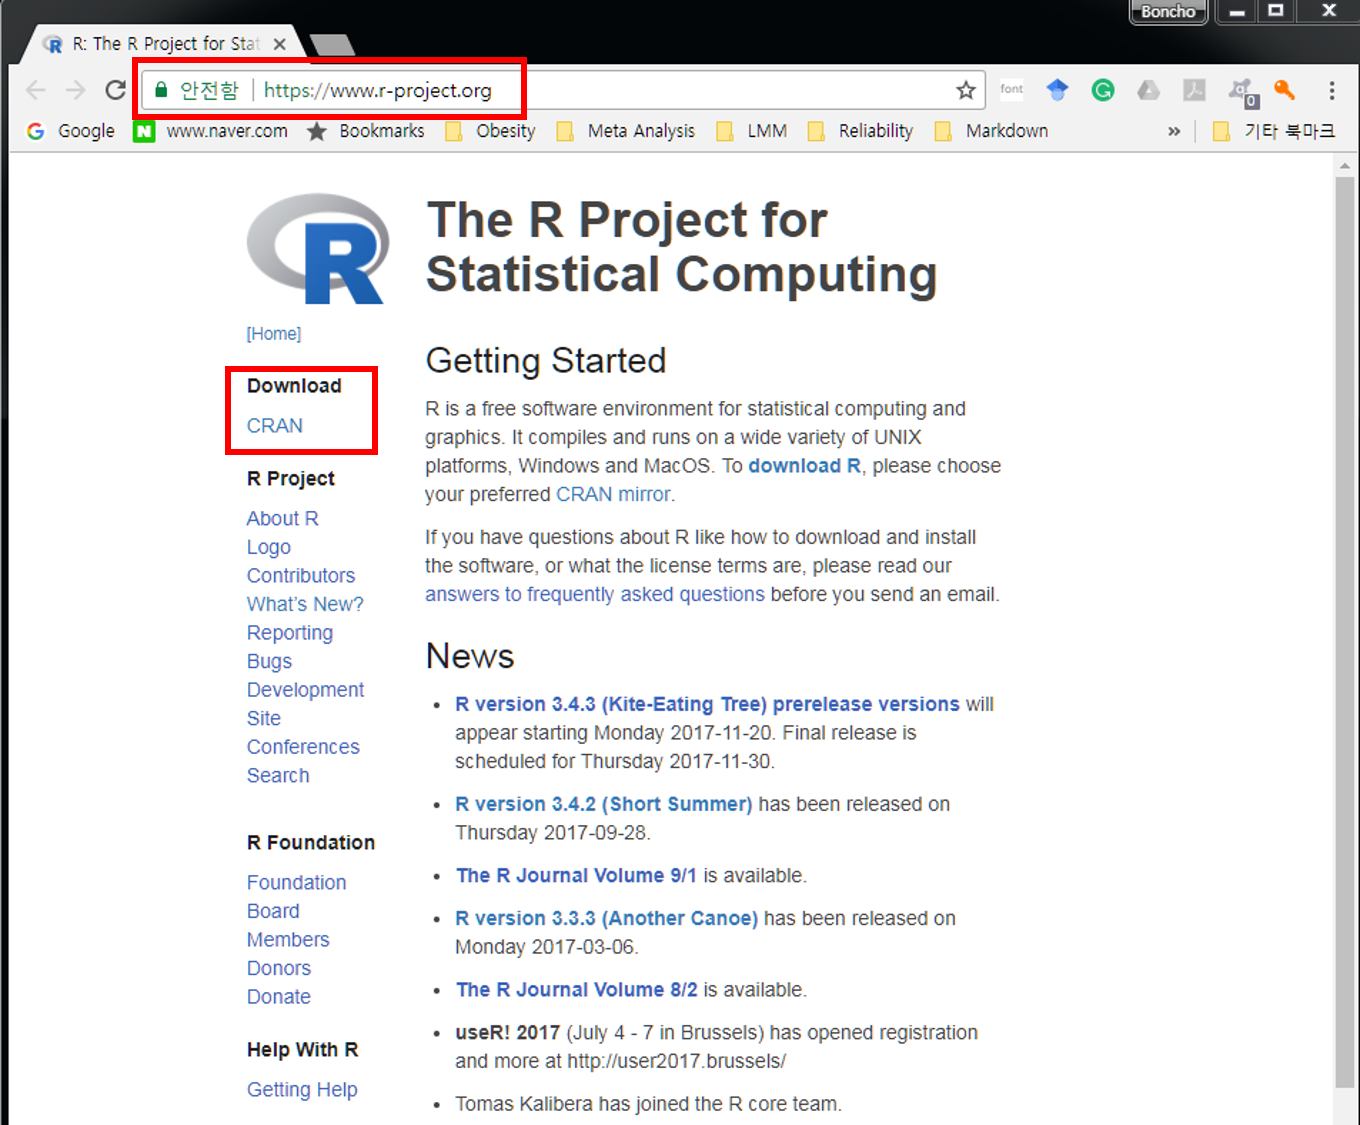
\includegraphics[width=0.9\linewidth]{figures/Rorg-main-add} \end{center}

\normalsize

\begin{enumerate}
\def\labelenumi{\arabic{enumi}.}
\setcounter{enumi}{2}
\tightlist
\item
  클릭 후 연결한 페이지를 스크롤 후 Korea 아래 링크\footnote{해당 링크들은 접속 시점에 따라 변경될 수 있음} 클릭
\end{enumerate}

\footnotesize

\begin{center}
\includegraphics[width=0.9\linewidth]{figures/CRAN-korea-01} \end{center}

\normalsize

\begin{enumerate}
\def\labelenumi{\arabic{enumi}.}
\setcounter{enumi}{3}
\tightlist
\item
  클릭 후 세 가지 운영체제(Linux, Mac OS X, Windowns)에 따른 R 버전 선택 가능\footnote{본 노트는 Windows 버전 설치만 다룸}
\end{enumerate}

\footnotesize

\begin{center}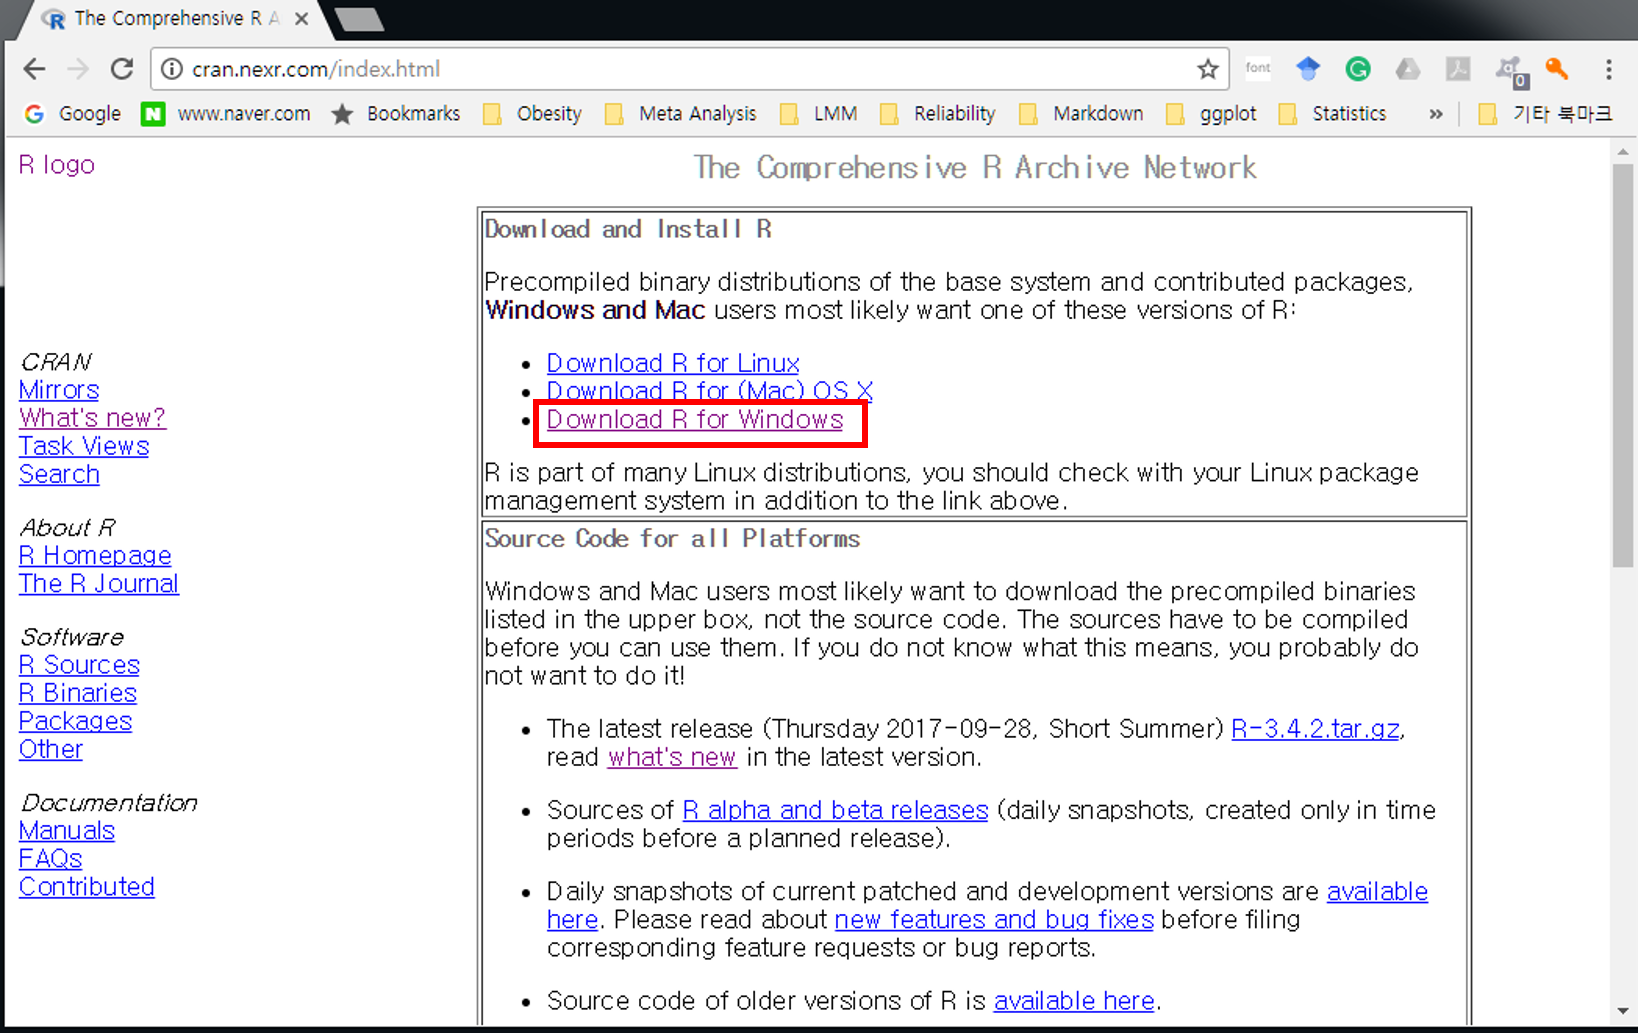
\includegraphics[width=0.9\linewidth]{figures/Rinstall-01} \end{center}

\normalsize

\begin{enumerate}
\def\labelenumi{\arabic{enumi}.}
\setcounter{enumi}{4}
\tightlist
\item
  \textbf{Downloads R for Windows} 링크 클릭하면 다음과 같은 화면으로 이동
\end{enumerate}

\footnotesize

\begin{center}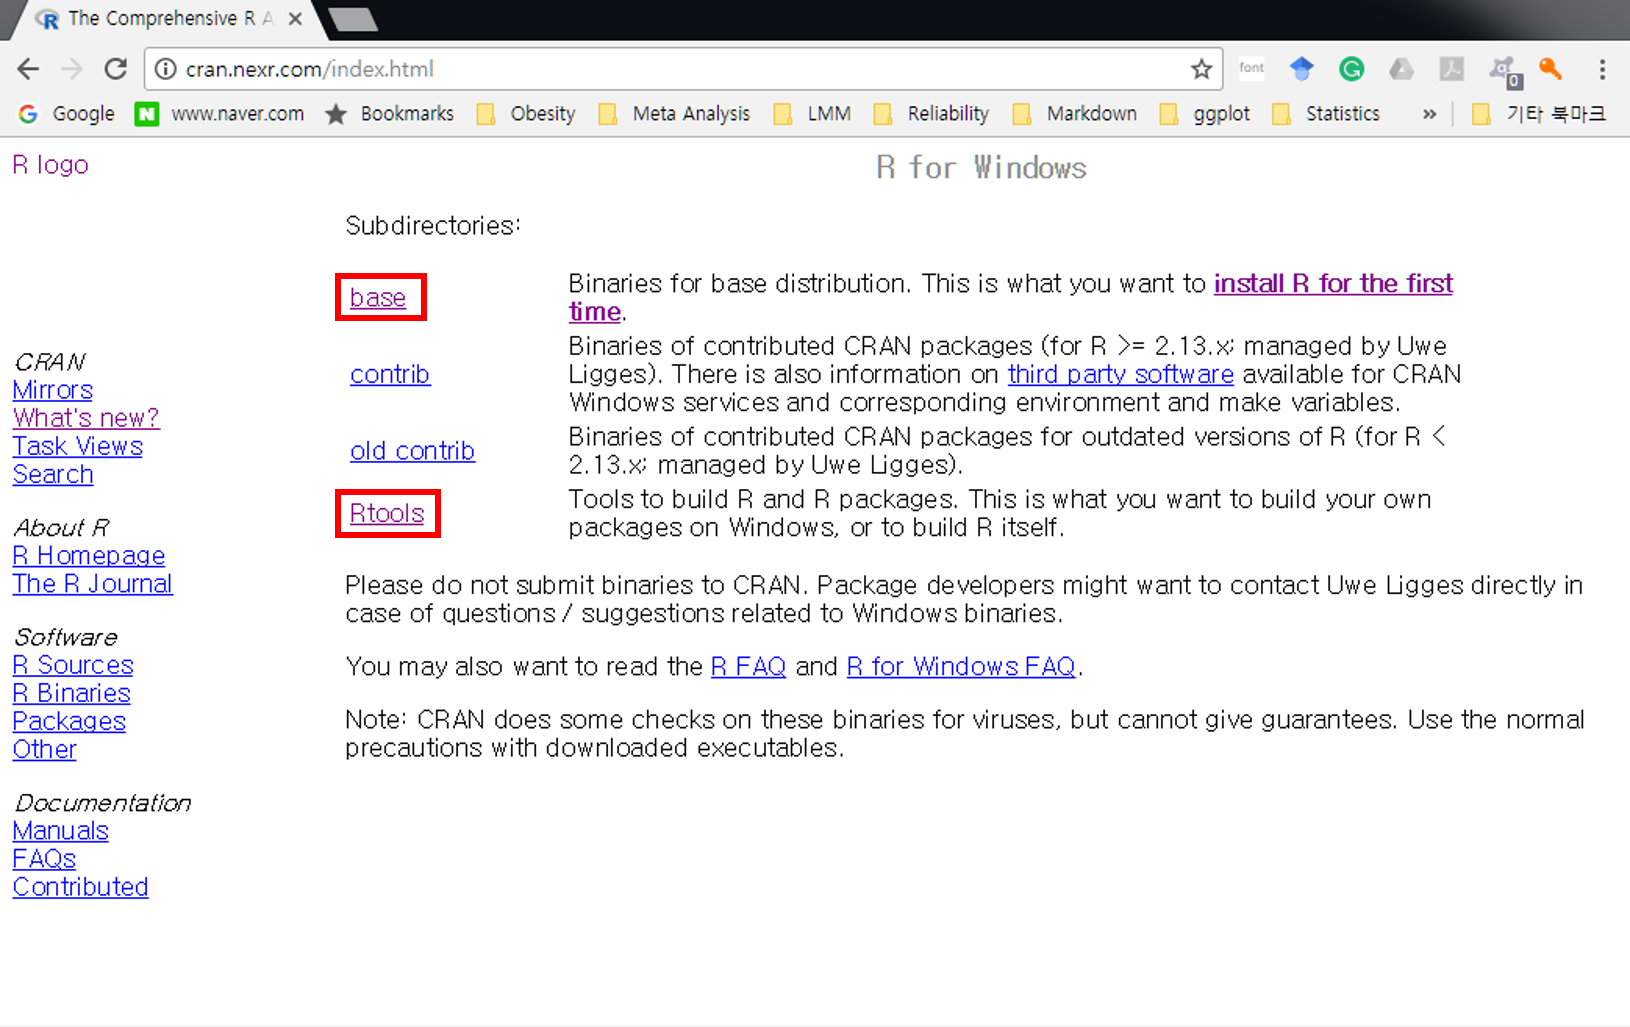
\includegraphics[width=0.9\linewidth]{figures/Rinstall-02} \end{center}

\normalsize

\footnotesize

\BeginKnitrBlock{rmdtip}
다음 하위폴더에 대한 간략 설멍

\begin{itemize}
\tightlist
\item
  \textbf{\texttt{base}}: R 실행 프로그램
\item
  \textbf{\texttt{contrib}}: R package의 바이너리 파일
\item
  \textbf{\texttt{Rtools}}: R package 개발 및 배포를 위한 프로그램
\end{itemize}
\EndKnitrBlock{rmdtip}

\normalsize

\begin{enumerate}
\def\labelenumi{\arabic{enumi}.}
\setcounter{enumi}{5}
\tightlist
\item
  위 화면에서 \textbf{base} 링크 클릭 후 아래 화면에서 \textbf{Downloads R 3.x.x for Windows} 를 클릭 후 설치 파일을 임의의 디렉토리에 저장 및 실행
\end{enumerate}

\footnotesize

\begin{center}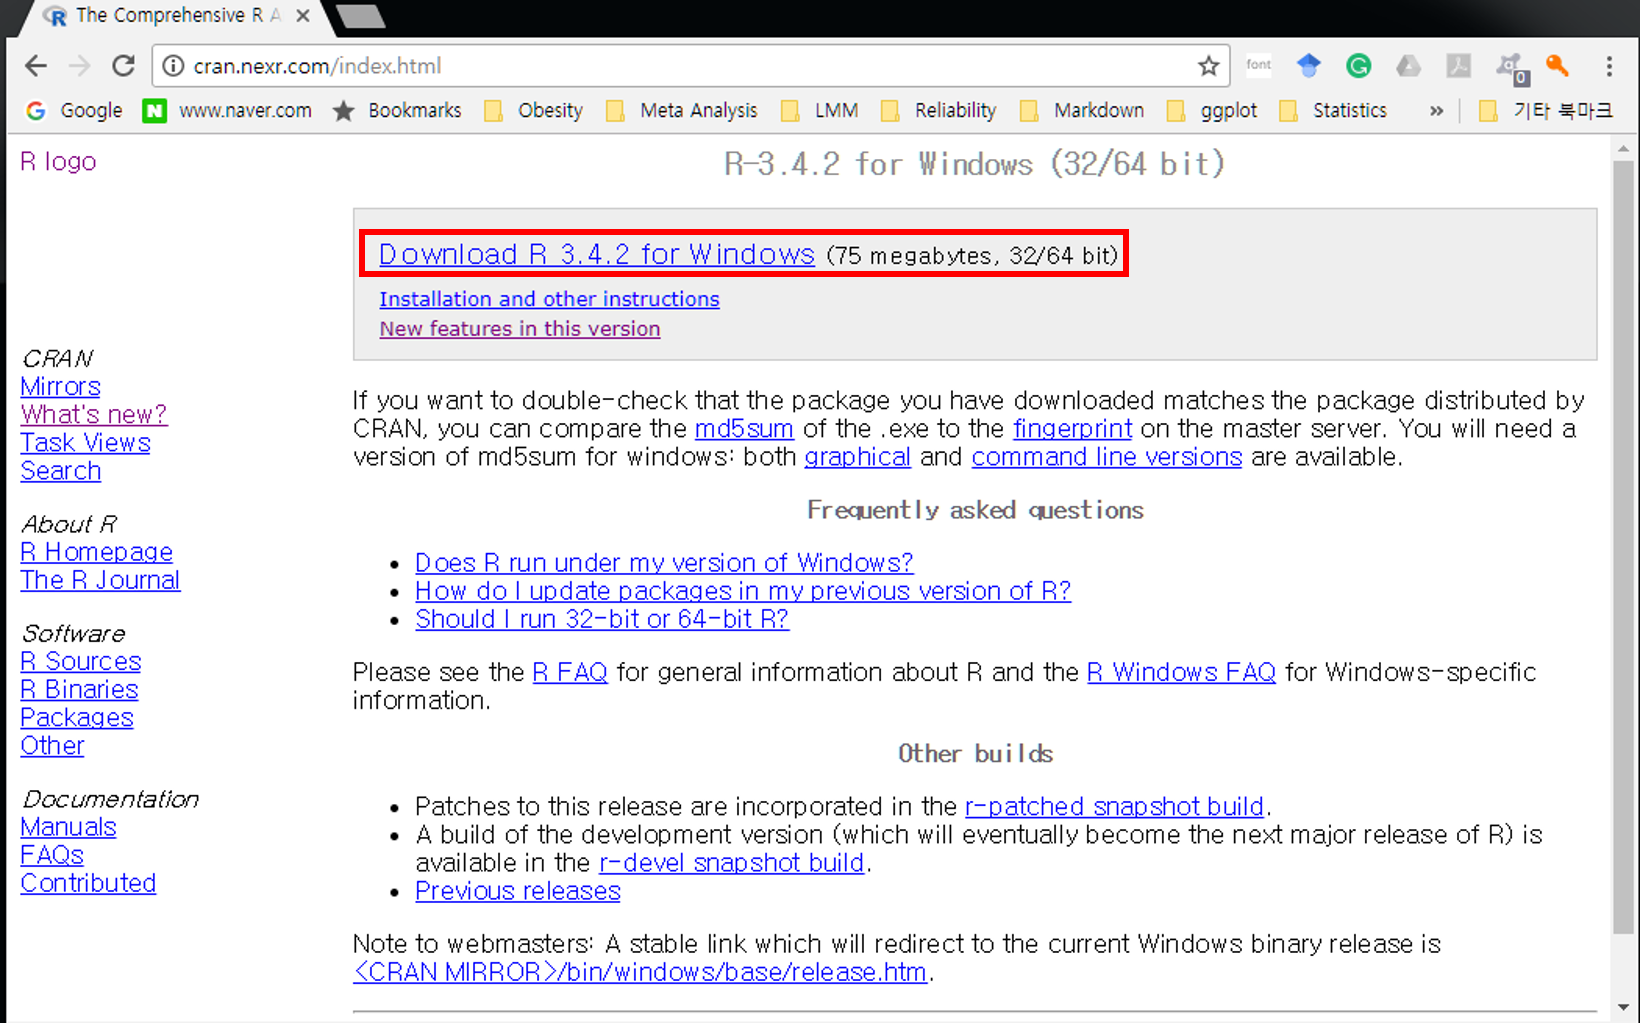
\includegraphics[width=0.9\linewidth]{figures/Rinstall-03} \end{center}

\normalsize

\begin{enumerate}
\def\labelenumi{\arabic{enumi}.}
\setcounter{enumi}{6}
\tightlist
\item
  다운로드한 파일을 실행하면 아래와 같은 대화창이 나타남

  \begin{itemize}
  \tightlist
  \item
    한국어 선택 \(\rightarrow\) 환영 화면에서 {[}다음(N)\textgreater{]} 클릭
  \end{itemize}
\end{enumerate}

\footnotesize

\begin{center}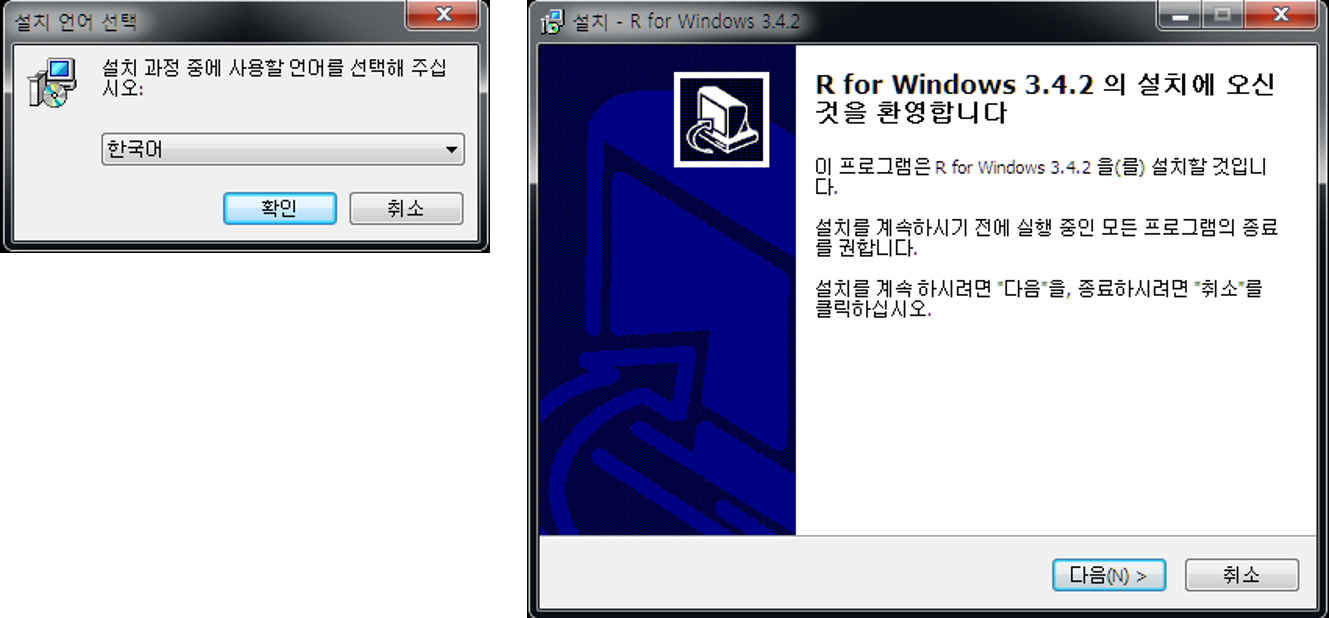
\includegraphics[width=0.9\linewidth]{figures/R-install-F01} \end{center}

\normalsize

\begin{enumerate}
\def\labelenumi{\arabic{enumi}.}
\setcounter{enumi}{7}
\tightlist
\item
  GNU 라이센스에 대한 설명 및 동의 여부({[}다음(N)\textgreater{]}) 클릭
\end{enumerate}

\footnotesize

\begin{center}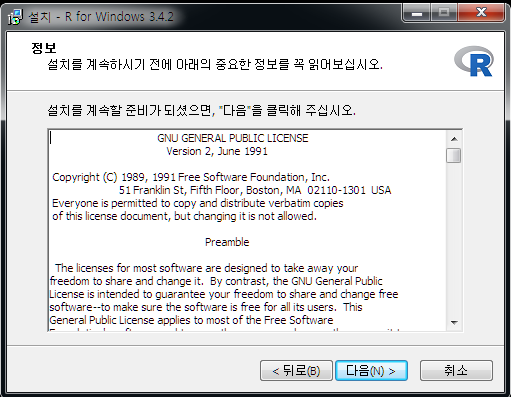
\includegraphics[width=0.9\linewidth]{figures/R-install-F02} \end{center}

\normalsize

\begin{enumerate}
\def\labelenumi{\arabic{enumi}.}
\setcounter{enumi}{8}
\tightlist
\item
  설치 디렉토리 설정 및 구성요소 설지 여부

  \begin{itemize}
  \tightlist
  \item
    원하는 디렉토리 설정(예: \texttt{C:\textbackslash{}R\textbackslash{}R-3.x.x})
  \item
    기본 프로그램(``Core Files''), 32 또는 64 bit 용 설치 파일, R console 한글 번역 모두 체크 뒤 {[}다음(N)\textgreater{]} 클릭
  \end{itemize}
\end{enumerate}

\footnotesize

\begin{center}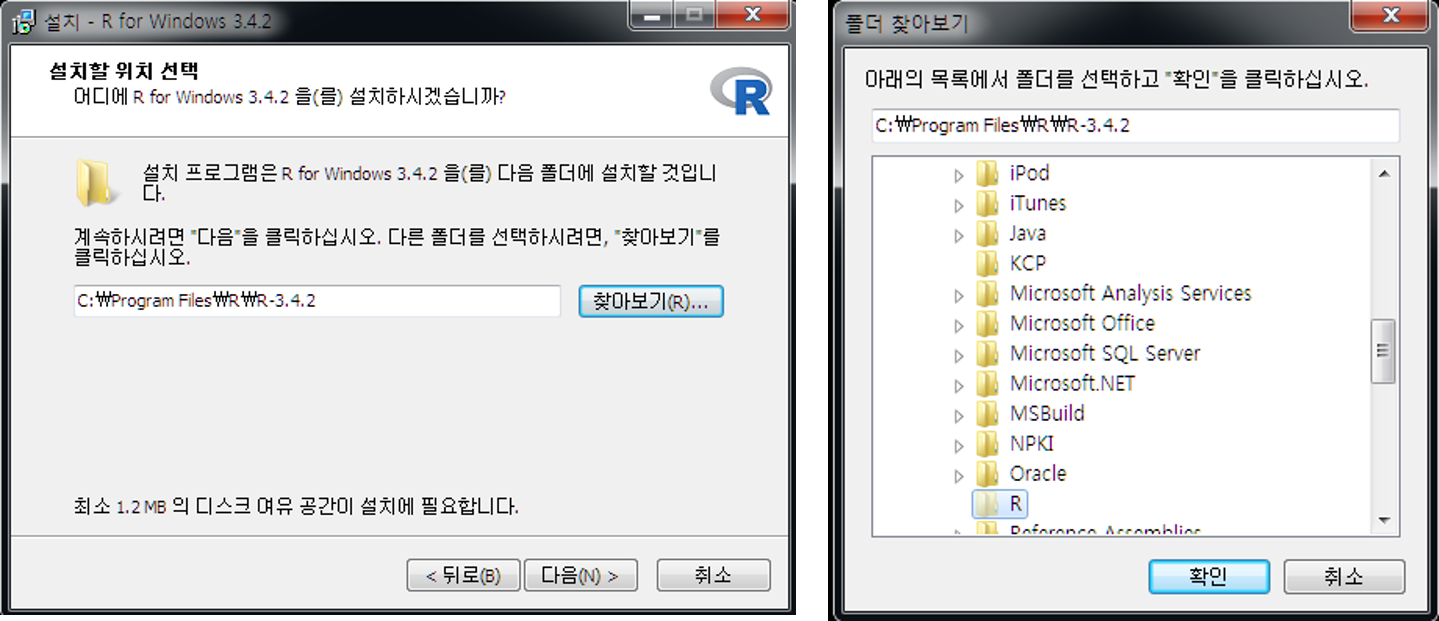
\includegraphics[width=0.9\linewidth]{figures/R-install-F03} \end{center}

\normalsize

\footnotesize

\begin{center}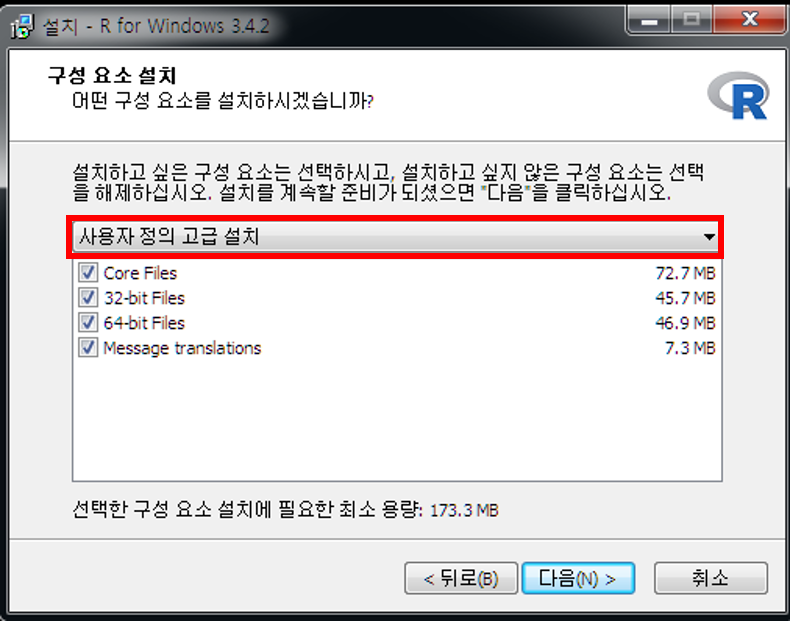
\includegraphics[width=0.9\linewidth]{figures/R-install-F04} \end{center}

\normalsize

\begin{enumerate}
\def\labelenumi{\arabic{enumi}.}
\setcounter{enumi}{9}
\tightlist
\item
  R 스타트업 옵션 지정
\end{enumerate}

\begin{itemize}
\tightlist
\item
  기본값(``No'' check-button)으로도 설치 진행 가능
\item
  본 문서에서는 스타트업 옵션 변경으로 진행
\end{itemize}

\footnotesize

\begin{center}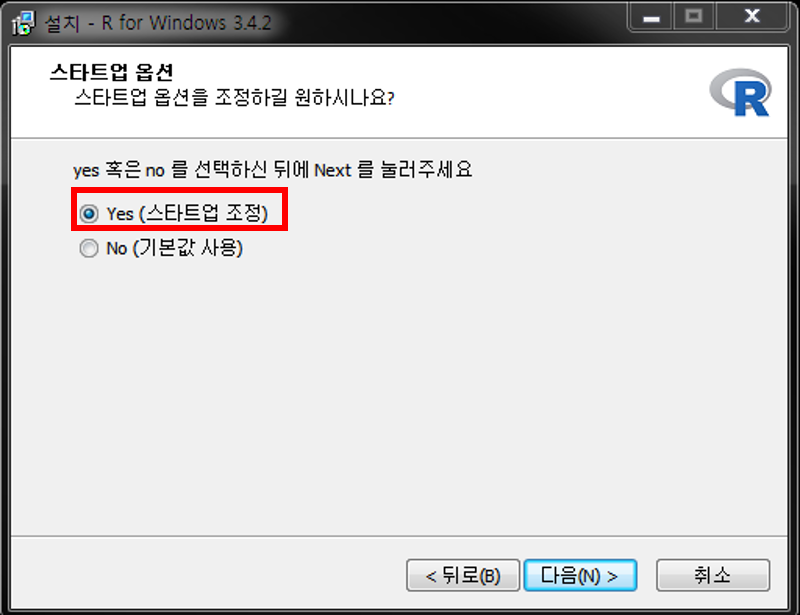
\includegraphics[width=0.9\linewidth]{figures/R-install-F05} \end{center}

\normalsize

\begin{enumerate}
\def\labelenumi{\arabic{enumi}.}
\setcounter{enumi}{10}
\tightlist
\item
  화면표시방식(디스플레이 모드) 설정 변경
\end{enumerate}

\begin{itemize}
\tightlist
\item
  MDI: 한 윈도우 내에서 script 편집창, 출력, 도움말 창 사용
\item
  SDI: 다중 창에서 각각 script 편집창, 출력, 도움말 등을 독립적으로 열기
\end{itemize}

\footnotesize

\begin{center}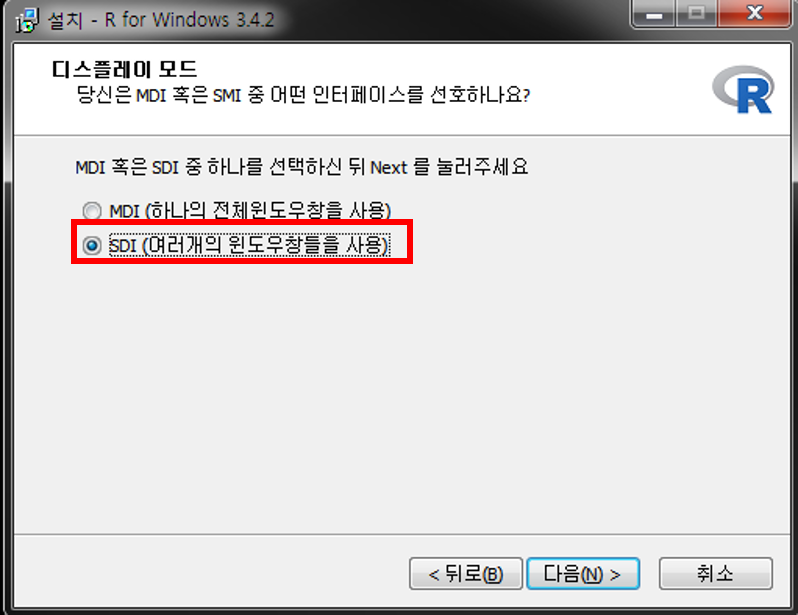
\includegraphics[width=0.9\linewidth]{figures/R-install-F06} \end{center}

\normalsize

\begin{enumerate}
\def\labelenumi{\arabic{enumi}.}
\setcounter{enumi}{11}
\tightlist
\item
  도움말 형식에서 HTML 도움말 기반 선택
\end{enumerate}

\footnotesize

\begin{center}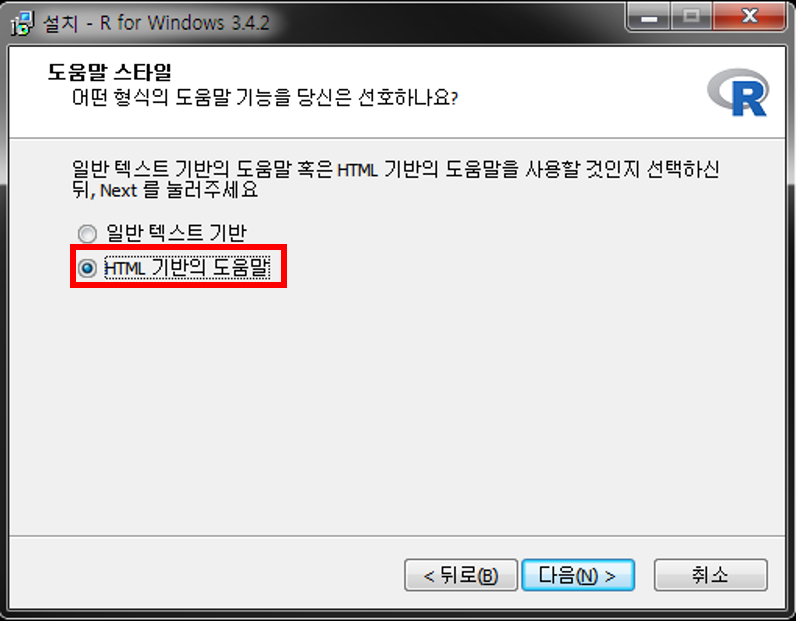
\includegraphics[width=0.9\linewidth]{figures/R-install-F07} \end{center}

\normalsize

\begin{enumerate}
\def\labelenumi{\arabic{enumi}.}
\setcounter{enumi}{12}
\tightlist
\item
  시작메뉴 폴더 선택
\end{enumerate}

\begin{itemize}
\tightlist
\item
  ``바로가기''를 생성할 시작 메뉴 폴더 지정 후 {[}다음(N)\textgreater{]} 클릭 후 설치 진행
\item
  하단 ``시작메뉴 폴더 만들지 않음'' 체크박스 표시 시 시작메뉴에 ``바로가기'' 아이콘이 생성되지 않음(실행에 전혀 지장 없음)
\end{itemize}

\footnotesize

\begin{center}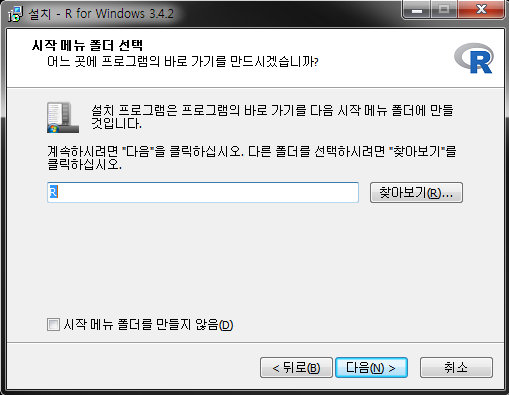
\includegraphics[width=0.9\linewidth]{figures/R-install-F08} \end{center}

\normalsize

\begin{enumerate}
\def\labelenumi{\arabic{enumi}.}
\setcounter{enumi}{13}
\tightlist
\item
  추가 옵션 지정: 바탕화면 아이콘 생성 등 추가적 작업 옵션 체크 후 {[}다음(N)\textgreater{]} 클릭 \(\rightarrow\) 설치 진행
\end{enumerate}

\begin{itemize}
\tightlist
\item
  설치된 R 버전 정보 레지스트리 저장 여부
\item
  \texttt{.Rdata} 확장자를 R 실행파일과 자동 연계
\end{itemize}

\footnotesize

\begin{center}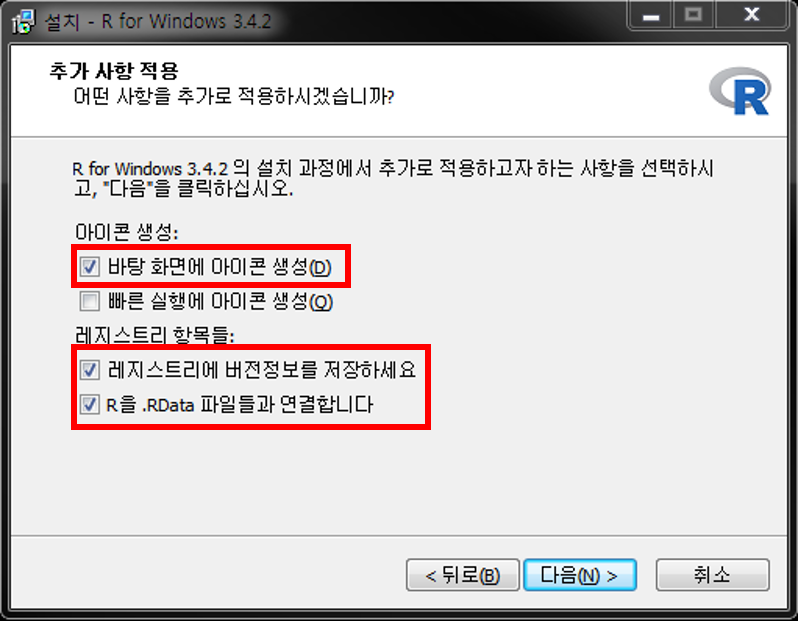
\includegraphics[width=0.9\linewidth]{figures/R-install-F09} \end{center}

\normalsize

\begin{enumerate}
\def\labelenumi{\arabic{enumi}.}
\setcounter{enumi}{14}
\tightlist
\item
  설치 완료 후 바탕화면의 R 아이콘을 더블클릭하면 Rgui가 실행
\end{enumerate}

\footnotesize

\begin{figure}

{\centering 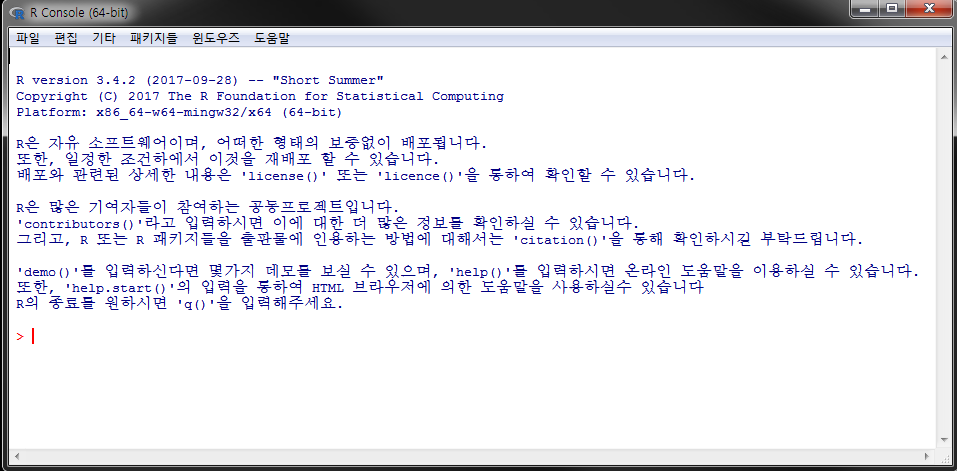
\includegraphics[width=1\linewidth]{figures/Rgui} 

}

\caption{Windows에서 R 실행화면(콘솔 창, SDI 모드)}\label{fig:r-console}
\end{figure}

\normalsize

\hypertarget{r-check}{%
\section{R 시작 및 작동 체크}\label{r-check}}

\BeginKnitrBlock{rmdimportant}
\textbf{실습}: 설치된 R을 실행 후 보이는 R 콘솔(consle) 창에서 명령어를 실행하고 결과 확인
\EndKnitrBlock{rmdimportant}

Figure \ref{fig:r-console} 에서 \texttt{\textgreater{}} 기호는 R의 명령 프롬프트(command prompt) 임

\begin{itemize}
\tightlist
\item
  \(\rightarrow\) 컴퓨터가 사용자 명령을 기다리고 있다는 기호
\end{itemize}

\begin{enumerate}
\def\labelenumi{\arabic{enumi}.}
\tightlist
\item
  현재 R session\footnote{현재 실행되고 있는 R의 작업공간} 정보(R 설치 버전, locale, 로딩 packages) 출력
\end{enumerate}

\footnotesize

\begin{Shaded}
\begin{Highlighting}[]
\CommentTok{# R의 설치 버전 및 현재 설정된 locale(언어, 시간대) 및 로딩된 R package 정보 출력}
\KeywordTok{sessionInfo}\NormalTok{() }
\end{Highlighting}
\end{Shaded}

\begin{verbatim}
R version 3.6.3 (2020-02-29)
Platform: x86_64-w64-mingw32/x64 (64-bit)
Running under: Windows 10 x64 (build 18363)

Matrix products: default

locale:
[1] LC_COLLATE=Korean_Korea.949  LC_CTYPE=Korean_Korea.949   
[3] LC_MONETARY=Korean_Korea.949 LC_NUMERIC=C                
[5] LC_TIME=Korean_Korea.949    

attached base packages:
[1] stats     graphics  grDevices utils     datasets  methods   base     

other attached packages:
[1] knitr_1.28

loaded via a namespace (and not attached):
 [1] compiler_3.6.3  magrittr_1.5    bookdown_0.18.1 htmltools_0.4.0
 [5] tools_3.6.3     yaml_2.2.1      Rcpp_1.0.4      stringi_1.4.6  
 [9] rmarkdown_2.1   stringr_1.4.0   digest_0.6.25   xfun_0.12      
[13] rlang_0.4.5     evaluate_0.14  
\end{verbatim}

\normalsize

\begin{enumerate}
\def\labelenumi{\arabic{enumi}.}
\setcounter{enumi}{1}
\tightlist
\item
  문자열 출력
\end{enumerate}

\footnotesize

\begin{Shaded}
\begin{Highlighting}[]
\CommentTok{#문자열 출력}
\KeywordTok{print}\NormalTok{(}\StringTok{"Hello R"}\NormalTok{) }\CommentTok{#문자열}
\end{Highlighting}
\end{Shaded}

\begin{verbatim}
[1] "Hello R"
\end{verbatim}

\normalsize

\begin{quote}
\texttt{\#} 기호는 주석의 시작을 의미하고 실제로 실행되지 않음 같은 행에서 \texttt{\#} 뒤 내용의 코드 역시 실행되지 않음
\end{quote}

\begin{enumerate}
\def\labelenumi{\arabic{enumi}.}
\setcounter{enumi}{2}
\tightlist
\item
  \texttt{a} 라는 변수에 숫자 9, \texttt{b}라는 변수에 숫자 7를 할당 후 출력
\end{enumerate}

\footnotesize

\begin{Shaded}
\begin{Highlighting}[]
\CommentTok{# 수치형 값(scalar)을 변수에 할당(assign)}
\CommentTok{# 여러 명령어를 한줄에 입력할 때에는 세미콜론(;)으로 구분}
\NormalTok{a =}\StringTok{ }\DecValTok{9}\NormalTok{; b =}\StringTok{ }\DecValTok{7}
\NormalTok{a}
\end{Highlighting}
\end{Shaded}

\begin{verbatim}
[1] 9
\end{verbatim}

\begin{Shaded}
\begin{Highlighting}[]
\NormalTok{b}
\end{Highlighting}
\end{Shaded}

\begin{verbatim}
[1] 7
\end{verbatim}

\normalsize

\begin{enumerate}
\def\labelenumi{\arabic{enumi}.}
\setcounter{enumi}{3}
\tightlist
\item
  변수 \texttt{a}와 \texttt{b}의 사칙연산
\end{enumerate}

\footnotesize

\begin{Shaded}
\begin{Highlighting}[]
\NormalTok{a}\OperatorTok{+}\NormalTok{b; a}\OperatorTok{-}\NormalTok{b; a}\OperatorTok{*}\NormalTok{b; a}\OperatorTok{/}\NormalTok{b}
\end{Highlighting}
\end{Shaded}

\begin{verbatim}
[1] 16
\end{verbatim}

\begin{verbatim}
[1] 2
\end{verbatim}

\begin{verbatim}
[1] 63
\end{verbatim}

\begin{verbatim}
[1] 1.285714
\end{verbatim}

\normalsize

\begin{enumerate}
\def\labelenumi{\arabic{enumi}.}
\setcounter{enumi}{4}
\tightlist
\item
  R 그래픽 맛보기: 정규분포로부터 난수 100개 생성 후 생성된 데이터에 대한 히스토그램 작성
\end{enumerate}

\footnotesize

\begin{Shaded}
\begin{Highlighting}[]
\CommentTok{# 난수 생성 시 값은 매번 달라지기 때문에 seed를 주어 일정값이 생성되도록 고정}
\CommentTok{# "="과 "<-"는 모두 동일한 기능을 가진 할당 연산자임}
\CommentTok{#평균이 0 이고 분산이 1인 정규분포에서 난수 100개 생성}
\KeywordTok{set.seed}\NormalTok{(}\DecValTok{12345}\NormalTok{) }\CommentTok{# random seed 지정}
\NormalTok{x <-}\StringTok{ }\KeywordTok{rnorm}\NormalTok{(}\DecValTok{100}\NormalTok{) }\CommentTok{# 난수 생성}
\KeywordTok{hist}\NormalTok{(x) }\CommentTok{# 히스토그램}
\end{Highlighting}
\end{Shaded}

\begin{figure}

{\centering 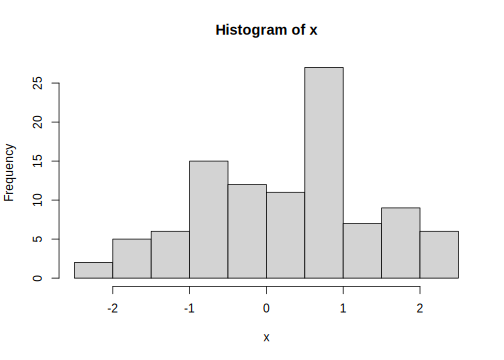
\includegraphics{01-overview_files/figure-latex/check-04-1} 

}

\caption{정규분포 100개의 히스토그램}\label{fig:check-04}
\end{figure}

\normalsize

\footnotesize

\BeginKnitrBlock{rmdtip}
R 명령어 또는 전체 프로그램 소스 실행 시 매우 빈번히 오류가 나타나는데, 이를 해결할 수 있는 가장 좋은 방법은 앞에서 언급한 Google을 이용한 검색 또는 R 설치 시 자체적으로 내장되어 있는 도움말을 참고하는 것이 가장 효율적임.
\EndKnitrBlock{rmdtip}

\normalsize

\footnotesize

\begin{table}[H]

\caption{\label{tab:tab-help}R help 관련 명령어 리스트}
\centering
\fontsize{10}{12}\selectfont
\begin{tabular}[t]{l>{\raggedright\arraybackslash}p{5cm}l}
\toprule
도움말 보기 명령어 & 설명 & 사용법\\
\midrule
\rowcolor{gray!6}  `help` 또는 `?` & 도움말 시스템 호출 & `help(함수명)`\\
`help.search` 또는 `??` & 주어진 문자열을 포함한 문서 검색 & `help.search(pattern)`\\
\rowcolor{gray!6}  `example` & topic의 도움말 페이지에 있는 examples section 실행 & `example(함수명)`\\
`vignette` & topic의 pdf 또는 html 레퍼런스 메뉴얼 불러오기 & `vignette(패키지명 또는 패턴)`\\
\bottomrule
\end{tabular}
\end{table}

\normalsize

\footnotesize

\BeginKnitrBlock{rmdtip}
\textbf{Vignette} 의 활용

\begin{itemize}
\tightlist
\item
  \texttt{vignette()}에서 제공하는 문서는 데이터를 기반으로 사용하고자 하는 패키지의 실제 활용 예시를 작성한 문서이기 때문에 초보자들이 R 패키지 활용에 대한 접근성을 높혀줌.
\item
  \texttt{browseVignettes()} 명령어를 통해 vignette을 제공하는 R 패키지 및 해당 vignette 문서 확인 가능
\end{itemize}
\EndKnitrBlock{rmdtip}

\normalsize

\hypertarget{rconsle-script}{%
\section{R script 편집기 사용}\label{rconsle-script}}

\BeginKnitrBlock{rmdimportant}
\textbf{실습}: R 설치 후 Rgui 에서 제공하는 편집기(R editor)에 명령어를 입력하고 실행
\EndKnitrBlock{rmdimportant}

설치된 R을 실행 후 상단 pull-down 메뉴에서 {[}\textbf{File}{]} \(\rightarrow\) {[}\textbf{새 스크립트}{]}를 선택하면 아래 그림과 같이 편집창(R 인스톨 시 SDI 옵션 기준)이 나타남

\footnotesize

\begin{center}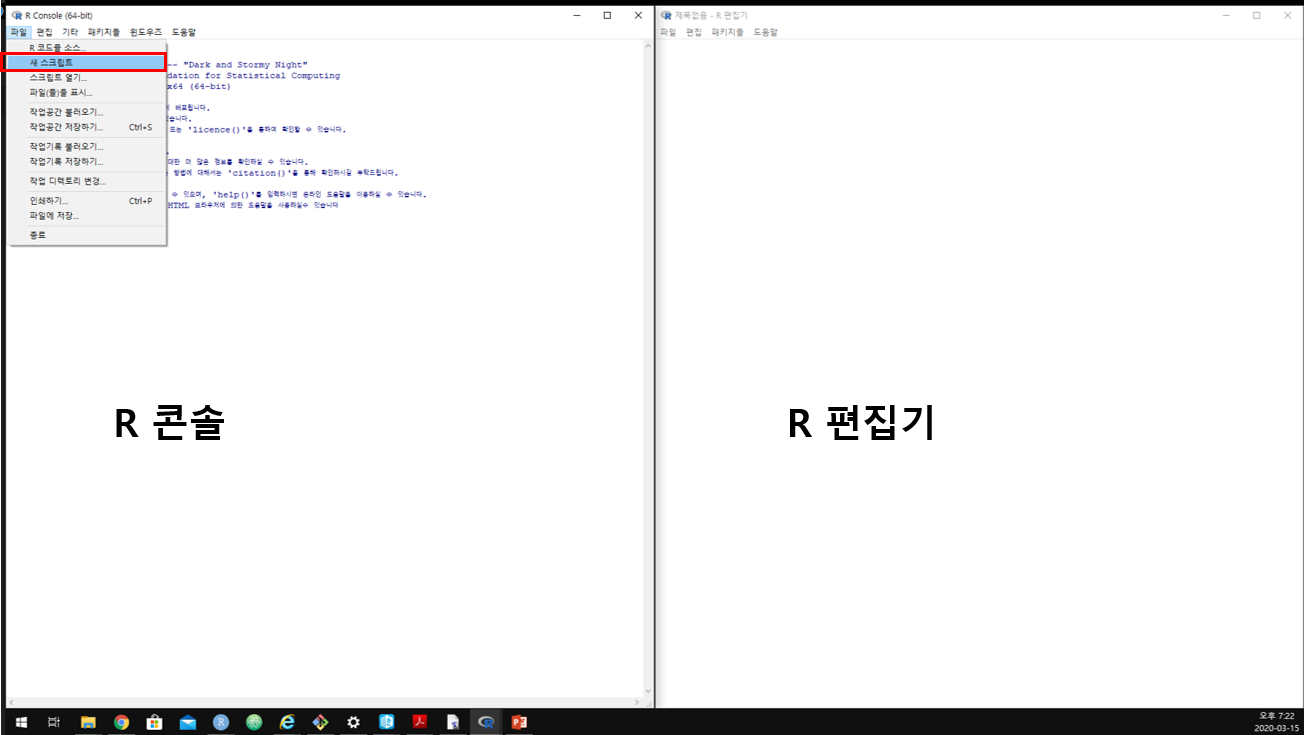
\includegraphics[width=1\linewidth]{figures/r-console-edit} \end{center}

\normalsize

편집기 창에 다음 명령어 입력

\footnotesize

\begin{Shaded}
\begin{Highlighting}[]
\CommentTok{# R에 내장된 cars 데이터셋 불러오기 cars dataset에 포함된 변수들의 기초통계량}
\CommentTok{# 출력 2차원 산점도}
\KeywordTok{data}\NormalTok{(cars)}
\KeywordTok{help}\NormalTok{(cars)  }\CommentTok{# cars 데이터셋에 대한 설명 help 창에 출력}
\KeywordTok{head}\NormalTok{(cars)  }\CommentTok{# cars 데이터셋 처음 6개 행 데이터 출력}
\KeywordTok{summary}\NormalTok{(cars)  }\CommentTok{# cars 데이터셋 요약}
\KeywordTok{plot}\NormalTok{(cars)  }\CommentTok{# 변수가 2개인 경우 산점도 출력}
\end{Highlighting}
\end{Shaded}

\normalsize

\begin{itemize}
\tightlist
\item
  편집창에서 한 줄을 실행시키려면 명령어가 입력된 줄에서 \textbf{{[}Ctrl{]}} + \textbf{{[}R{]}} 입력
\item
  편집창에 입력한 모든 명령어를 실행시키려면 모든 줄을 선택(마우스 또는 {[}Shift{]} + \(\downarrow\))
\end{itemize}

\footnotesize

\begin{verbatim}
  speed dist
1     4    2
2     4   10
3     7    4
4     7   22
5     8   16
6     9   10
\end{verbatim}

\begin{verbatim}
     speed           dist       
 Min.   : 4.0   Min.   :  2.00  
 1st Qu.:12.0   1st Qu.: 26.00  
 Median :15.0   Median : 36.00  
 Mean   :15.4   Mean   : 42.98  
 3rd Qu.:19.0   3rd Qu.: 56.00  
 Max.   :25.0   Max.   :120.00  
\end{verbatim}

\begin{figure}
\centering
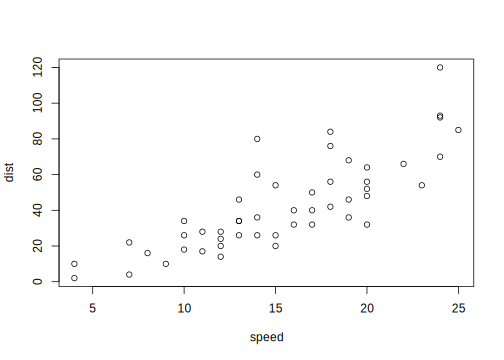
\includegraphics{01-overview_files/figure-latex/check-edit-out-1.pdf}
\caption{\label{fig:check-edit-out}cars 데이터셋의 speed와 dist 간 2차원 산점도: speed는 자동차 속도(mph)이고 dist는 해당 속도에서 브레이크를 밟았을 때 멈출 때 까지 걸린 거리(ft)를 나타냄.}
\end{figure}

\normalsize

\begin{itemize}
\tightlist
\item
  R은 명령어를 입력하고 실행결과를 확인하는 대화형(interpreter) 방식
\item
  콘솔창에서 \(\uparrow\)/\(\downarrow\)를 누르면 이전/이후 실행 명령 기록 확인 가능
\item
  여러 줄 이상 R 명령어라든가 반복적, 장기간 작업을 수행해야 할 경우 R 명령어로 구성된 스크립트 작성 후 일괄 실행하는 것이 일반적
\item
  여러 다중 명령 코딩 시 콘솔창에 직접 입력하는 것은 비효율적이므로 스크립트 에디터를 사용
\item
  위 예시처럼 R 에디터 사용할 수 있으나 가독성 및 코딩 효율이 떨어짐
\item
  과거 많이 사용됐던 R 에디터: \href{http://www.winedt.com}{WinEdt}, \href{https://sourceforge.net/projects/tinn-r/}{Tinn-R}, \href{http://www.vim.org/scripts/script.php?script_id=2628}{Vim}
\item
  현재 가장 범용적 R 에디터: \textbf{Rstudio}
\end{itemize}

\hypertarget{r-studio}{%
\section{RStudio}\label{r-studio}}

\begin{itemize}
\tightlist
\item
  \href{https://rstudio.com/}{RStudio}: R 통합 분석/개발 환경(integrated development environment, IDE)으로 현재 가장 대중적으로 사용되고 있는 R 사용 환경
\item
  명령 곤솔 외 파일 편집, 데이터 객체, 명령 기록(.history), 그래프 등에 쉽게 접근 가능
\item
  RStudio 독자적인 개발 환경 제공: Rmarkdown, Rnotebook, Shiny Web Application 등 다양한 R 환경을 제공
\item
  버전관리(git, subversion)를 통해 project 관리 가능
\item
  \textbf{무료} 및 유료 소프트웨어 제공
\end{itemize}

\hypertarget{rstudio-install}{%
\subsection{RStudio 설치하기}\label{rstudio-install}}

\begin{enumerate}
\def\labelenumi{\arabic{enumi}.}
\tightlist
\item
  웹 브라우저를 통해 \url{https://rstudio.com} 접속 후 상단 \href{https://rstudio.com/products/rstudio/download/}{DOWNLOAD} 링크 클릭
\end{enumerate}

\footnotesize

\begin{center}
\includegraphics[width=0.8\linewidth]{figures/rstudio-homepage} \end{center}

\normalsize

\begin{enumerate}
\def\labelenumi{\arabic{enumi}.}
\setcounter{enumi}{1}
\item
  Desktop 또는 Server 버전 중 택일

  \begin{itemize}
  \tightlist
  \item
    서버용 설치를 위해서는 Server 클릭 \(\rightarrow\) 소규모 자료 분석용으로는 불필요
  \item
    여기서는 \textbf{Desktop} 버전 선택 후 다음 링크로 이동
  \end{itemize}
\end{enumerate}

\footnotesize

\begin{center}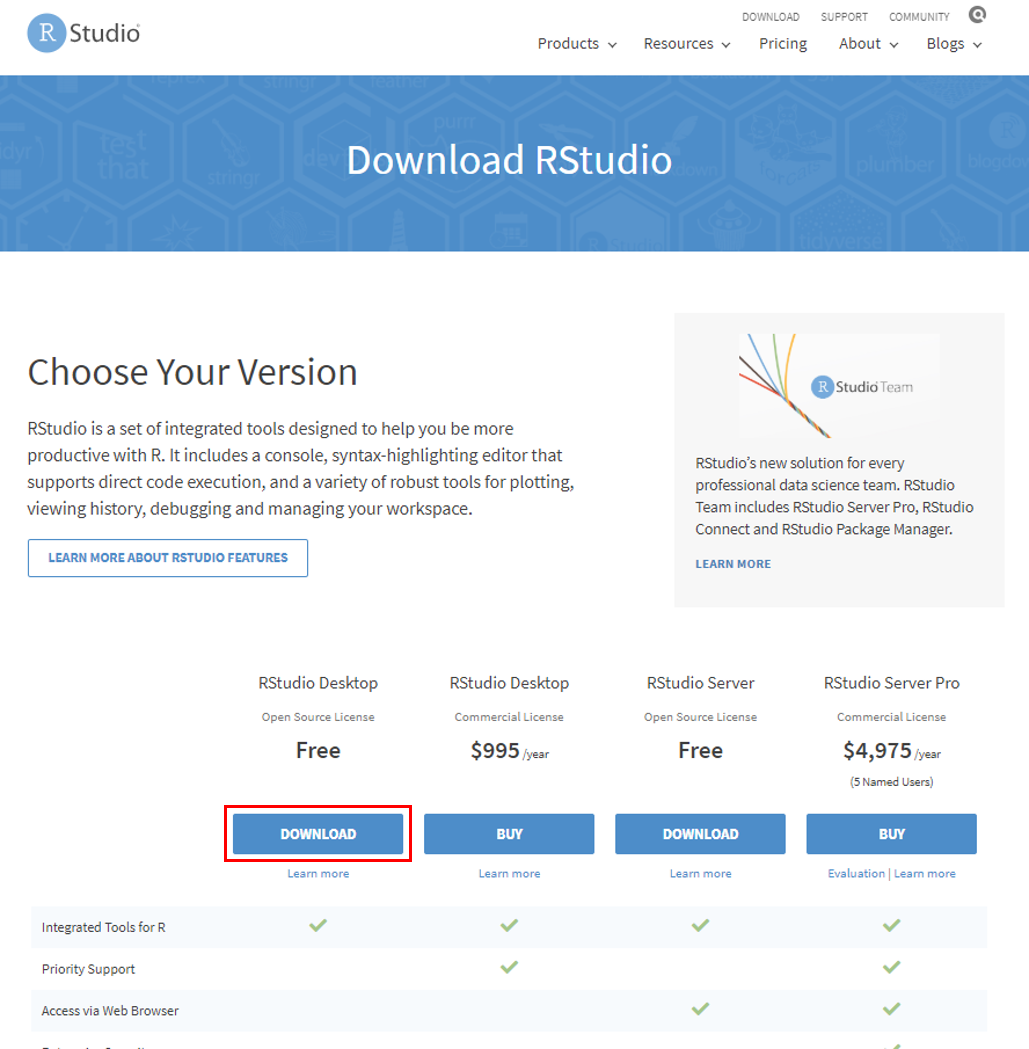
\includegraphics[width=0.7\linewidth]{figures/rstudio-download} \end{center}

\normalsize

\begin{enumerate}
\def\labelenumi{\arabic{enumi}.}
\setcounter{enumi}{2}
\tightlist
\item
  운영체제에 맞는 Rstudio installer 다운로드(여기서는 Windows 버전 다운로드)
\end{enumerate}

\footnotesize

\begin{center}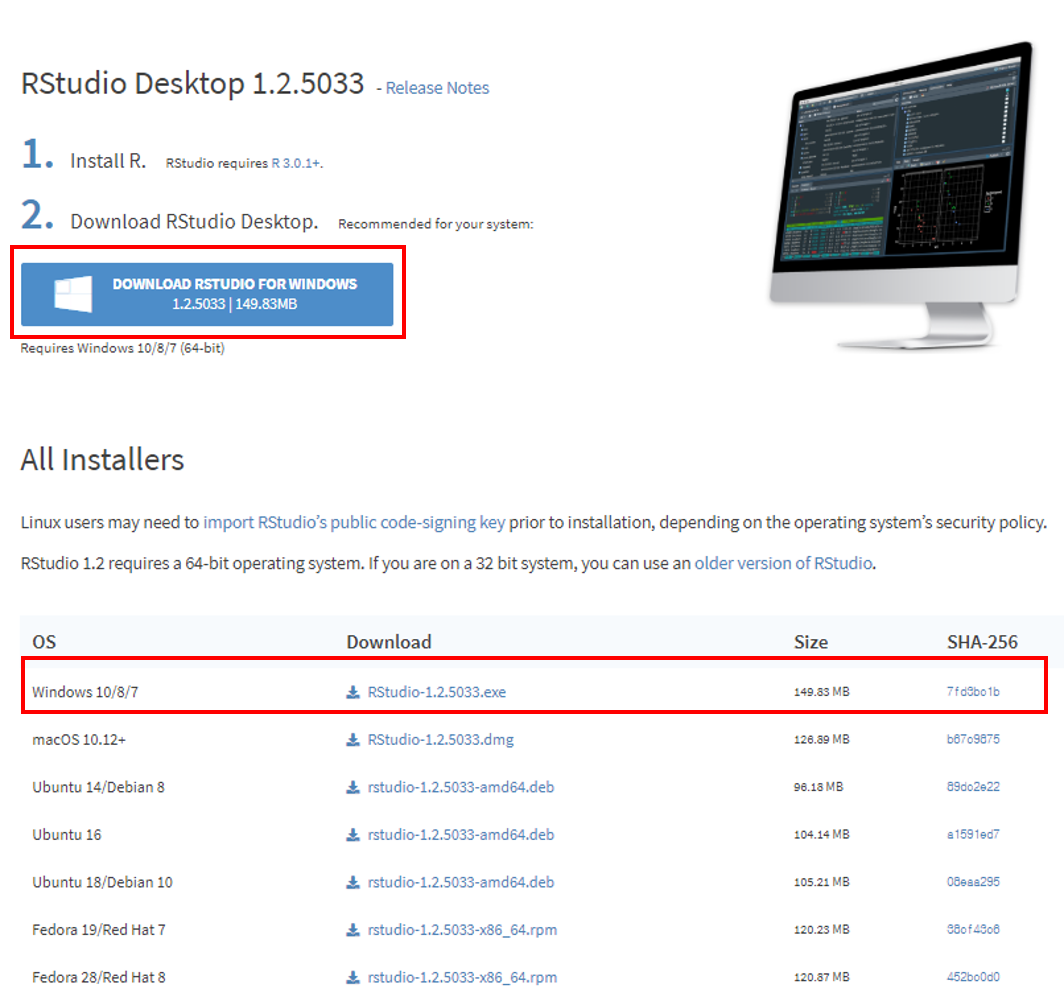
\includegraphics[width=0.6\linewidth]{figures/r-studio-download-02} \end{center}

\normalsize

\begin{enumerate}
\def\labelenumi{\arabic{enumi}.}
\setcounter{enumi}{3}
\tightlist
\item
  RStudio installer 다운로드 시 파일이 저장된 폴더에서 보통 \texttt{RStudio-xx.xx.xxx.exe} 형식의 파일명 확인

  \begin{itemize}
  \tightlist
  \item
    더블 클릭 후 실행
  \item
    \textbf{{[}다음\textgreater{]}} 몇 번 클릭 후 설치 종료
  \end{itemize}
\end{enumerate}

\footnotesize

\begin{center}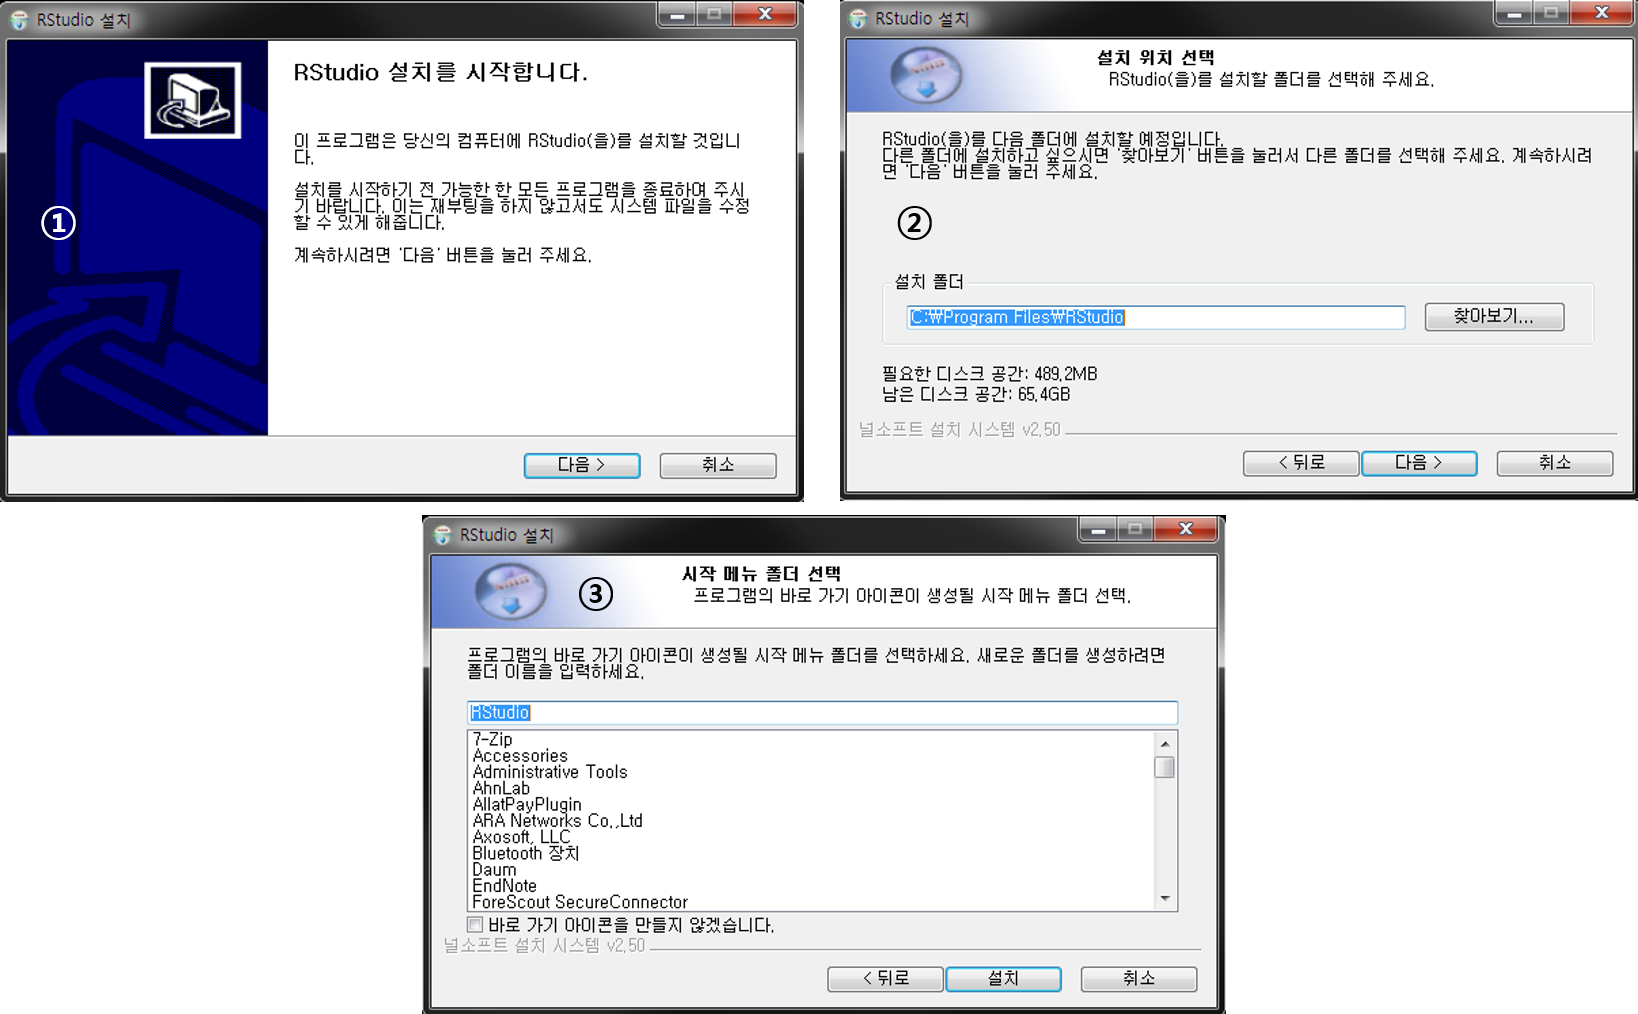
\includegraphics{figures/Rstudio-installer} \end{center}

\normalsize

\begin{enumerate}
\def\labelenumi{\arabic{enumi}.}
\setcounter{enumi}{4}
\tightlist
\item
  바탕화면 혹은 시작 프로그램에 새로 설치된 RStudio 아이콘 클릭 후 아래와 같은 프로그램 창이 나타나면 설치 성공
\end{enumerate}

\footnotesize

\begin{center}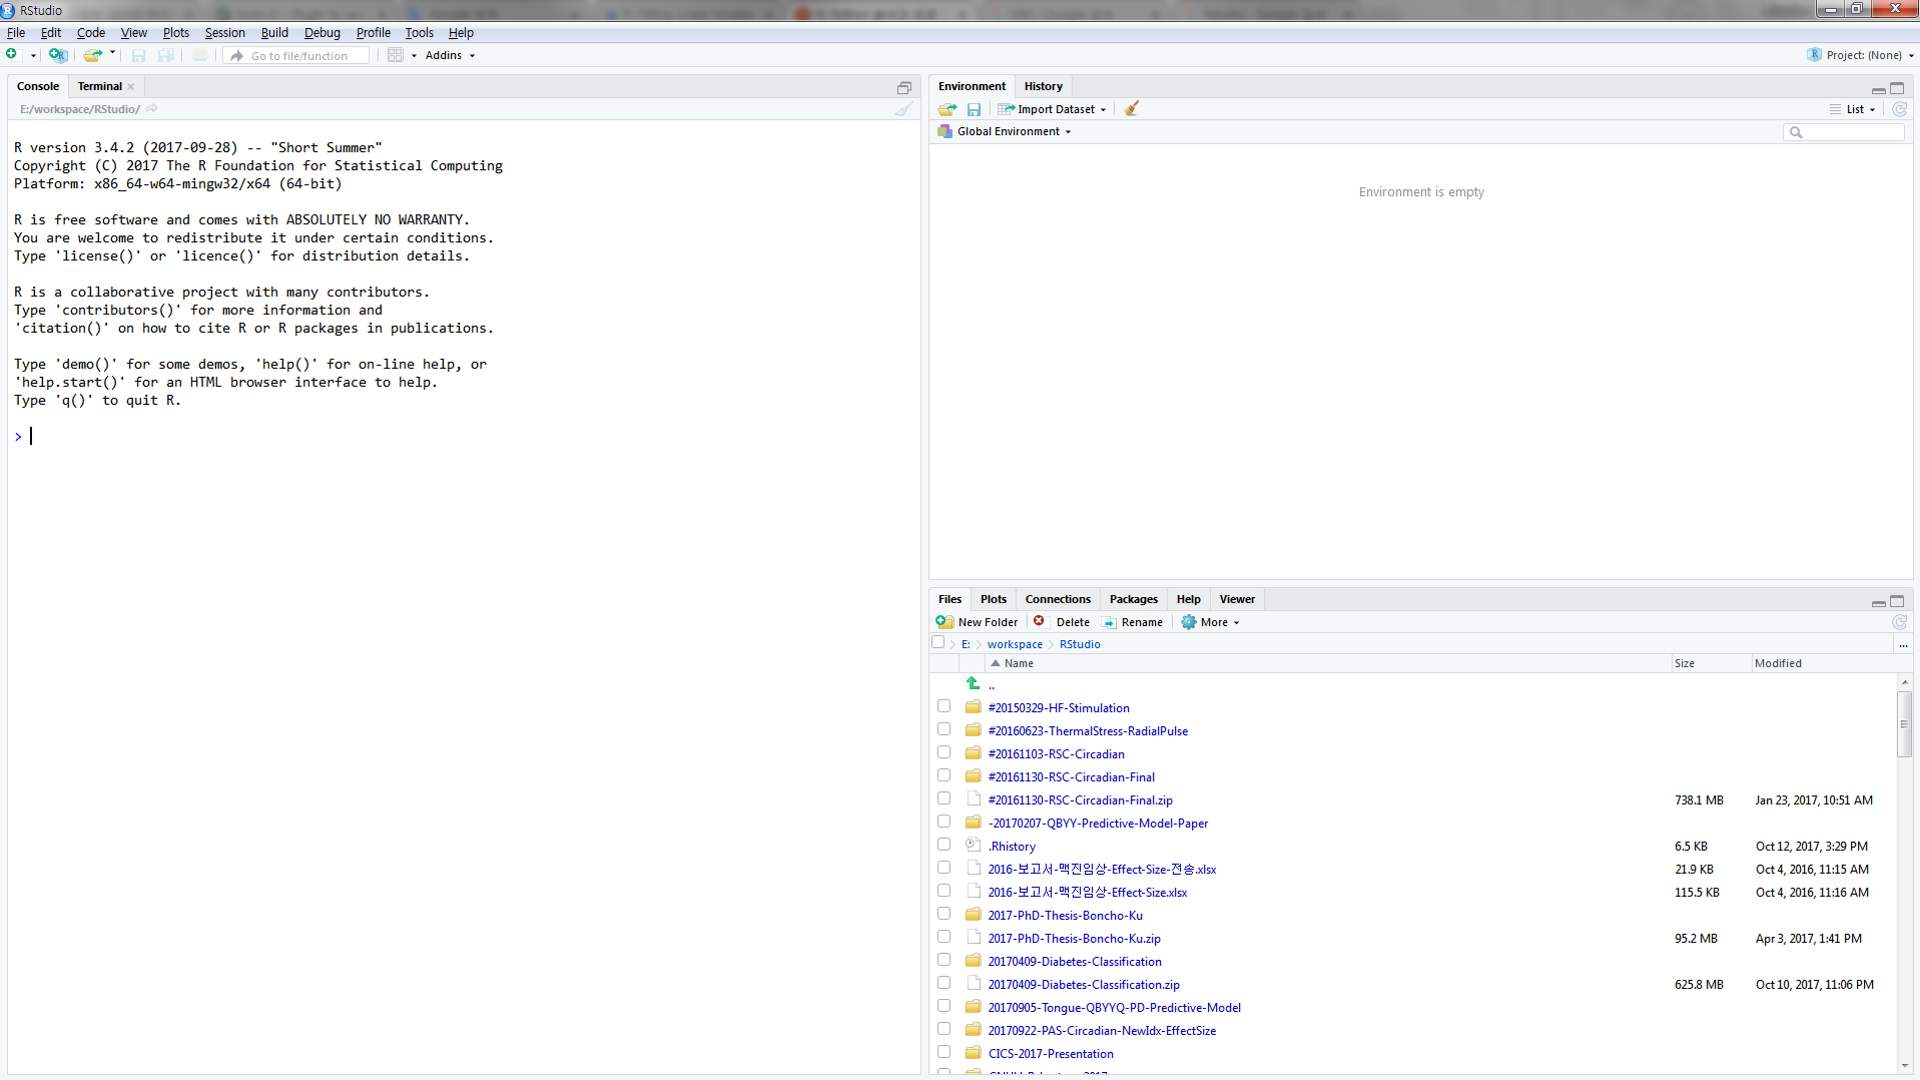
\includegraphics[width=0.8\linewidth]{figures/Rstudio-init} \end{center}

\normalsize

\hypertarget{rstudio-component}{%
\subsection{RStudio IDE 화면 구성}\label{rstudio-component}}

RStudio는 아래 그림과 같이 4개 창으로 구성\footnote{각 창의 위치는 세팅 구성에 따라 달라질 수 있음. 창 구성 방법은 RStudio 환경 옵션 설정에서 설명함.}

\footnotesize

\begin{figure}

{\centering 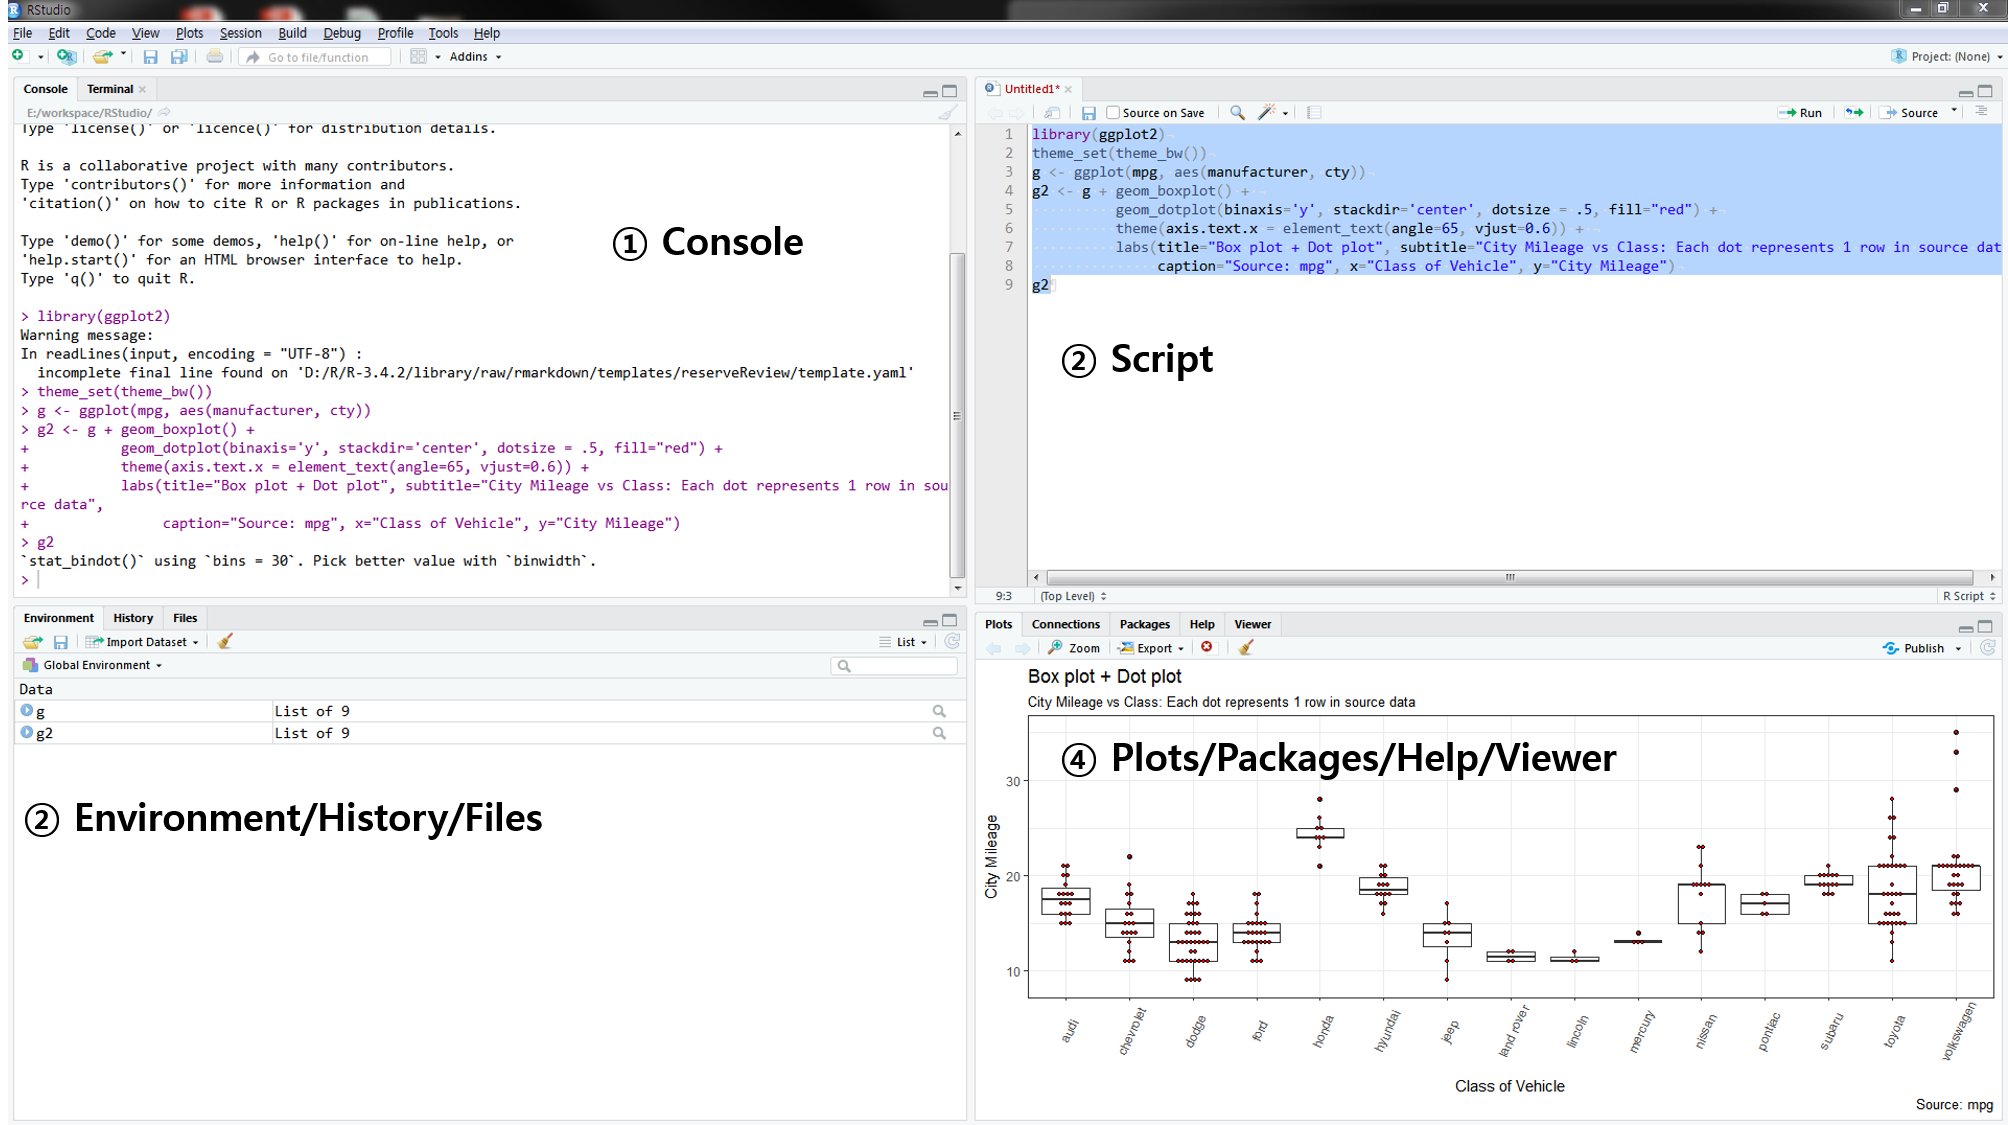
\includegraphics[width=0.9\linewidth]{figures/Rstudio-cap1} 

}

\caption{RStudio 화면구성: 우하단 그림은 http://r-statistics.co/Top50-Ggplot2-Visualizations-MasterList-R-Code.html 에서 발췌}\label{fig:rstudio-windows}
\end{figure}

\normalsize

\textbf{1. 콘솔(console)}

\begin{itemize}
\tightlist
\item
  R 명령어 실행공간(RGui, 정확하게는 R 설치 디렉토리에서 ``\textasciitilde/R/R.x.x/bin/x64/Rterm.exe'' 가 구동되고 있는 공간)
\item
  R script 또는 콘솔 창에서 작성한 명령어(프로그램) 실행 및 그 결과 출력
\item
  경고, 에러/로그 등의 메세지 확인
\end{itemize}

\footnotesize

\begin{figure}

{\centering 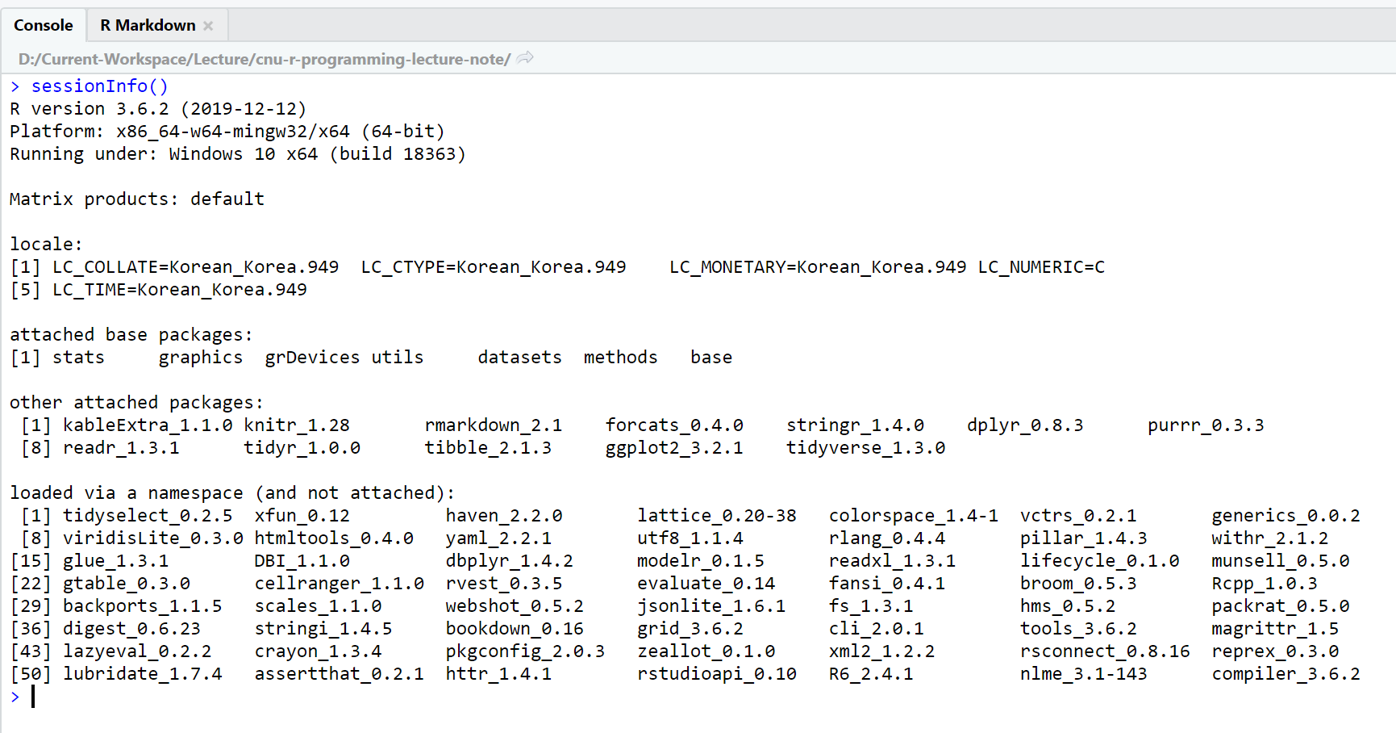
\includegraphics[width=0.8\linewidth]{figures/rstudio-console} 

}

\caption{RStudio 콘솔창에서 명령어 실행 후 출력결과 화면}\label{fig:rstudio-console}
\end{figure}

\normalsize

\textbf{2. 스크립트(script)} (Figure \ref{fig:rstudio-new-script})

\begin{itemize}
\tightlist
\item
  R 명령어 입력 공간으로 일괄처리(batch processing) 가능
\item
  새로운 스크립트 창 열기

  \begin{itemize}
  \tightlist
  \item
    아래 그림과 같이 pull-down 메뉴 좌측 상단 아이콘 클릭 후 {[}R script{]} 선택
  \item
    \texttt{{[}File{]}} \(\rightarrow\) \texttt{{[}New\ File{]}} \(\rightarrow\) \texttt{{[}R\ Script{]}} 선택
  \item
    단축 키: \texttt{{[}Ctrl{]}\ +\ {[}Shift{]}\ +\ {[}N{]}}
  \end{itemize}
\item
  일괄 명령어 처리를 위한 RStudio 제공 단축 키

  \begin{itemize}
  \tightlist
  \item
    \texttt{{[}Ctrl{]}\ +\ {[}Enter{]}}: 선택한 블럭 내 명령어 실행
  \item
    \texttt{{[}Alt{]}\ +\ {[}Enter{]}}: 선택 없이 커서가 위치한 라인의 명령어 실행
  \end{itemize}
\item
  R 스크립트 이외 R Markdown, R Notebook, Shiny web application 등 새 문서의 목적에 따라 다양한 종류의 소스 파일 생성 가능
\item
  저장된 R 스크립트 파일은 \texttt{파일명.R}로 저장됨
\item
  파일 실행 방법

  \begin{itemize}
  \tightlist
  \item
    실행하고자 하는 파일을 읽은 후(\texttt{{[}File{]}} \(\rightarrow\) \texttt{{[}Open\ File{]}} + 파일명 선택 또는 \texttt{파일명.R} 더블 클릭) 입력된 모든 라인을 선택한 뒤 \texttt{{[}Ctrl{]}\ +\ {[}Enter{]}}
  \item
    파일 읽은 후 \texttt{{[}Ctrl{]}\ +\ {[}Shift{]}\ +\ {[}S{]}} (현재 열려있는 \texttt{*.R} 파일에 대해) 또는 \texttt{{[}Ctrl{]}\ +\ {[}Shift{]}\ +\ {[}Enter{]}}
  \end{itemize}
\end{itemize}

\footnotesize

\begin{figure}

{\centering 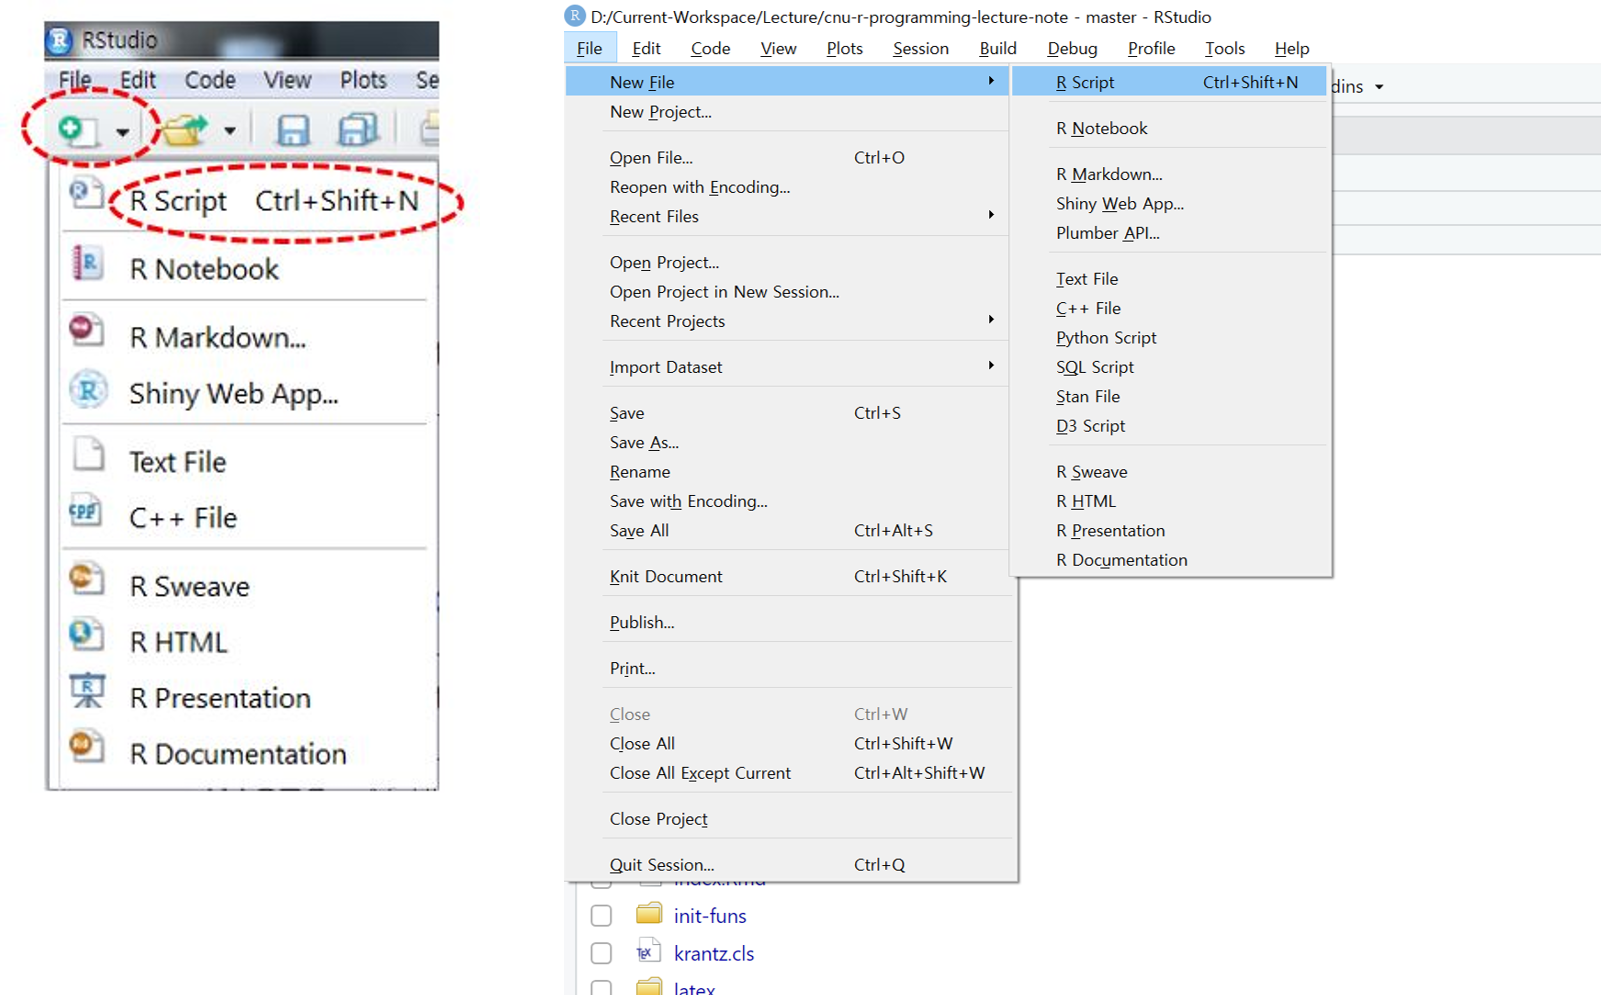
\includegraphics[width=0.8\linewidth]{figures/rstudio-open-new-script} 

}

\caption{RStudio 스크립트 새로 열기}\label{fig:rstudio-new-script}
\end{figure}

\normalsize

\footnotesize

\BeginKnitrBlock{rmdtip}
RStudio는 코딩 및 소스 작성의 효율성을 위해 여러 가지 단축 키를 제공하고 있음. 단축키는 아래 그림과 같이 pull down 메뉴 \texttt{{[}Tools{]}} 또는 \texttt{{[}Help{]}}에서 \texttt{{[}Keyboard\ shortcut\ help{]}} 또는 \texttt{{[}Alt{]}\ +\ {[}Shift{]}\ +\ {[}K{]}} 단축키를 통해 확인할 수 있음. 또는 Rstudio cheatsheet에서 단축키에 대한 정보를 제공하는데 pull down 메뉴 \texttt{{[}Help{]}} \(\rightarrow\) \texttt{{[}Cheatsheets{]}} \(\rightarrow\) \texttt{{[}RStudio\ IDE\ Cheat\ Sheet{]}}을 선택하면 각 아이콘 및 메뉴 기능에 대한 개괄적 설명 확인 가능함.
\EndKnitrBlock{rmdtip}

\normalsize

\textbf{3. 환경/명령기록(Environment/History)} (Figure \ref{fig:rstudio-env})

\begin{itemize}
\tightlist
\item
  \textbf{Environment}: 현재 R 작업환경에 저장되어 있는 객체의 특성 및 값 등을 요약 제시

  \begin{itemize}
  \tightlist
  \item
    좌측 아래 화살표 버튼 클릭: 해당 객체의 상세 정보 확인
  \item
    우측 사각형 버튼 또는 객체(데이터셋명) 클릭: 객체가 데이터셋(데이터프레임)인 경우 스프레드 시트 형태로 데이터셋 확인
  \end{itemize}
\end{itemize}

\footnotesize

\begin{figure}

{\centering 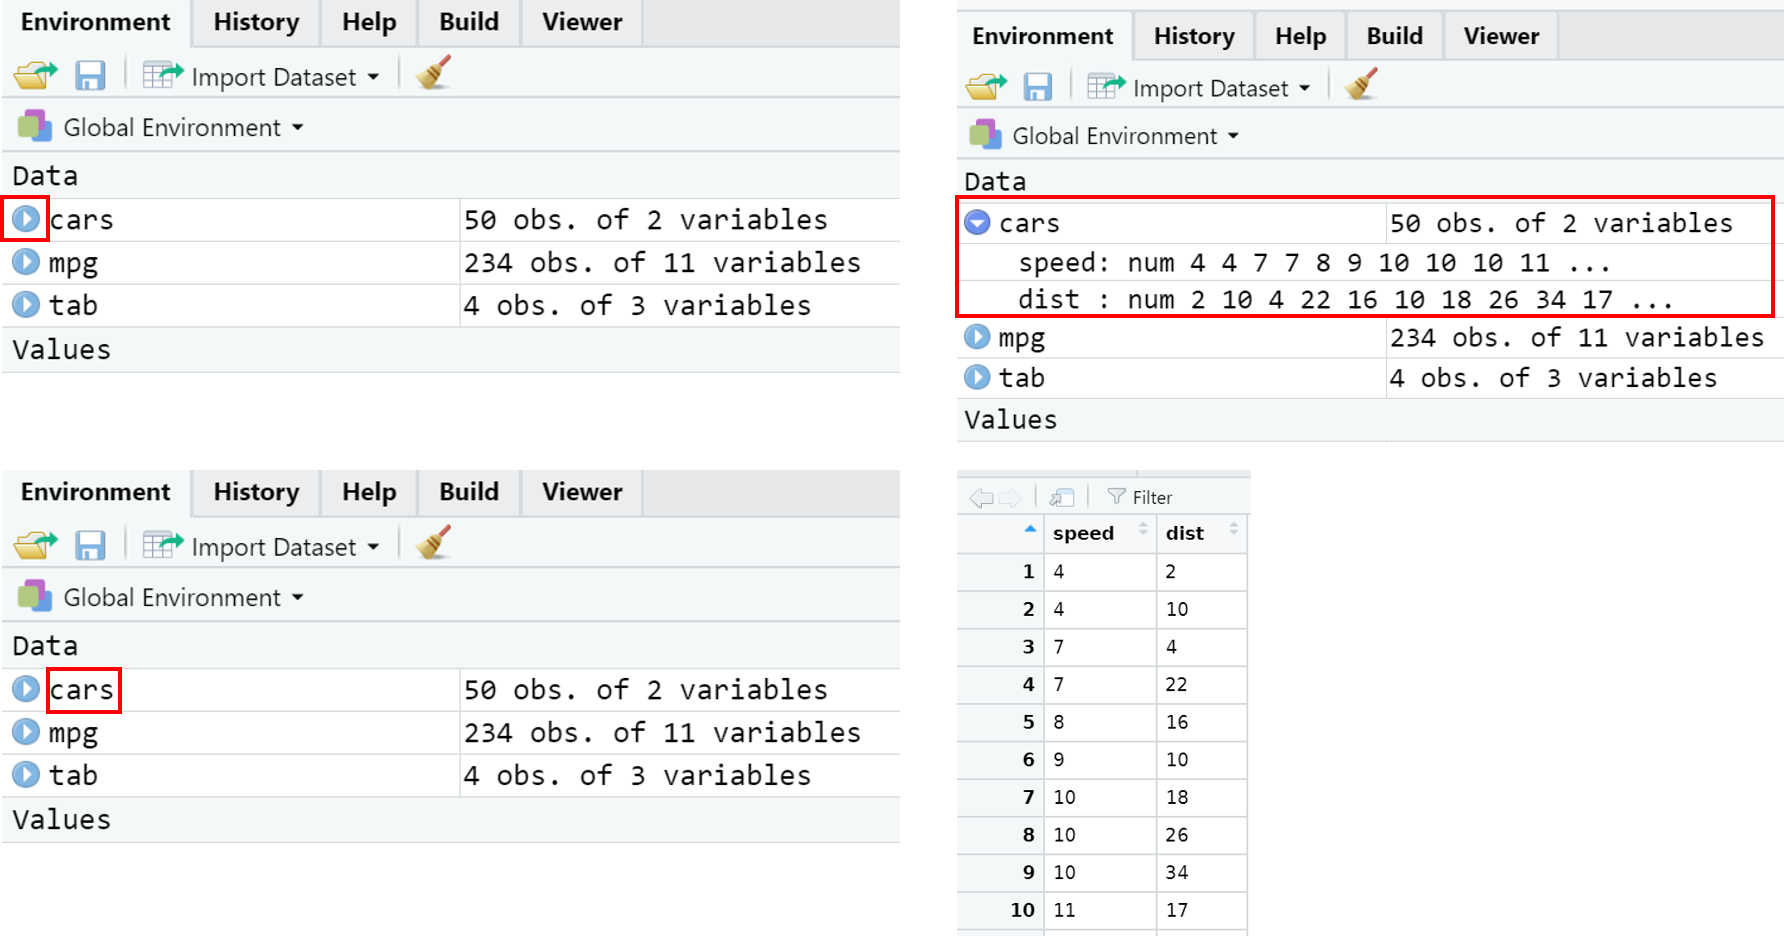
\includegraphics[width=0.9\linewidth]{figures/rstudio-environment} 

}

\caption{RStudio Environment 창 객체 상세 정보 및 스프레드 시트 출력 결과}\label{fig:rstudio-env}
\end{figure}

\normalsize

\begin{itemize}
\tightlist
\item
  History: R 콘솔에서 실행된 명령어(스크립트)들의 이력 확인
\end{itemize}

\footnotesize

\begin{center}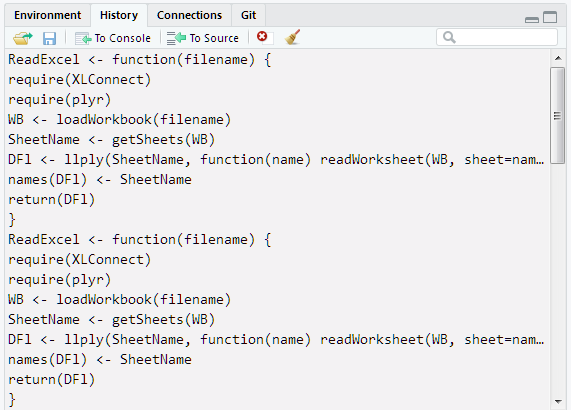
\includegraphics[width=0.9\linewidth]{figures/Rstudio-historywin} \end{center}

\normalsize

\textbf{4. File/Plots/Packages/Help/Viewer}

\begin{itemize}
\tightlist
\item
  File: Windows 파일 탐색기와 유사한 기능 제공

  \begin{itemize}
  \tightlist
  \item
    파일 및 폴더 생성, 삭제/파일 및 폴더명 수정, 그리고 작업경로 설정
  \end{itemize}
\end{itemize}

\footnotesize

\begin{center}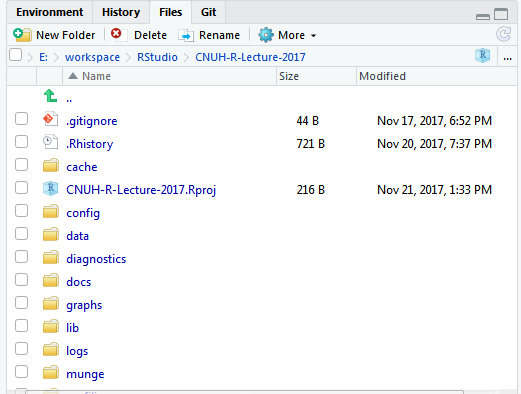
\includegraphics[width=0.8\linewidth]{figures/Rstudio-file} \end{center}

\normalsize

\begin{itemize}
\tightlist
\item
  \textbf{Plots}: 생성한 그래프 출력

  \begin{itemize}
  \tightlist
  \item
    작업 중 생성한 그래프 이력이 Plots 창에 저장: \(\leftarrow\) 이전, \(\rightarrow\) 최근
  \item
    \textbf{\texttt{Zoom}}: 클릭 시 해당 그래프의 팝업창이 생성되고 팝업창의 크기 조정을 통해 그래프의 축소/확대 가능
  \item
    \textbf{\texttt{Export}}: 선택한 그래프를 이미지 파일(\texttt{.png}, \texttt{.jpeg}, \texttt{.pdf} 등)로 저장할 수 있고, 클립보드로 복사 가능
  \end{itemize}
\end{itemize}

\footnotesize

\begin{center}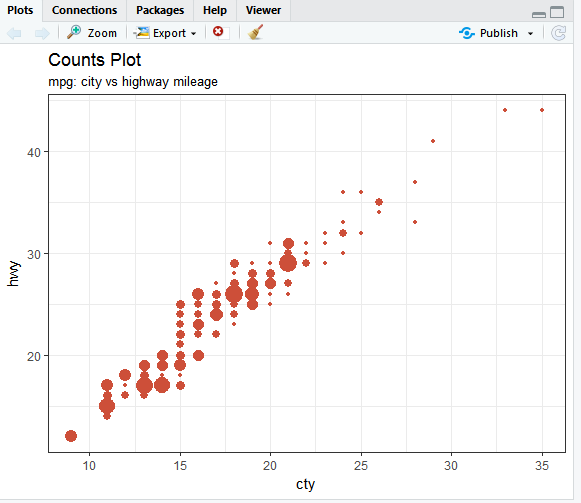
\includegraphics[width=0.8\linewidth]{figures/RStudio-plotwin} \end{center}

\normalsize

\begin{itemize}
\tightlist
\item
  \textbf{Packages}: 현재 컴퓨터에 설치된 R 패키지 목록 출력

  \begin{itemize}
  \tightlist
  \item
    신규 설치 및 업데이트 가능
  \end{itemize}
\end{itemize}

\footnotesize

\begin{center}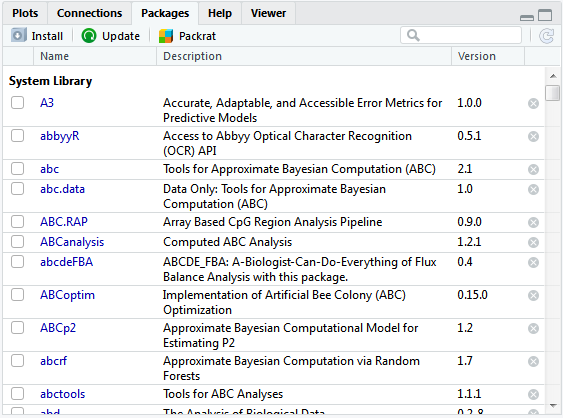
\includegraphics[width=0.8\linewidth]{figures/RStudio-packagewin} \end{center}

\normalsize

\begin{itemize}
\tightlist
\item
  \textbf{Help}: \texttt{help(topic)} 입력 시 도움말 창이 출력되는 공간
\end{itemize}

\footnotesize

\begin{Shaded}
\begin{Highlighting}[]
\KeywordTok{help}\NormalTok{(lm)}
\end{Highlighting}
\end{Shaded}

\normalsize

\footnotesize

\begin{center}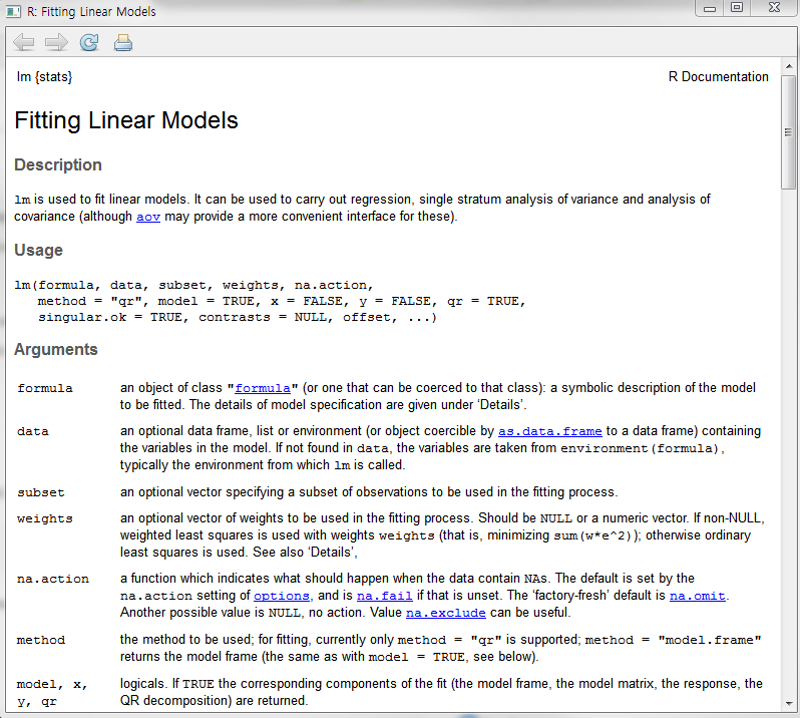
\includegraphics[width=0.8\linewidth]{figures/RStudio-helpwin} \end{center}

\normalsize

\hypertarget{rstudio-glob-options}{%
\subsection{RStudio 환경 설정}\label{rstudio-glob-options}}

Pull-down 메뉴에서 \texttt{{[}Tools{]}} \(\rightarrow\) \texttt{{[}Global\ Options...{]}}를 선택

\footnotesize

\begin{center}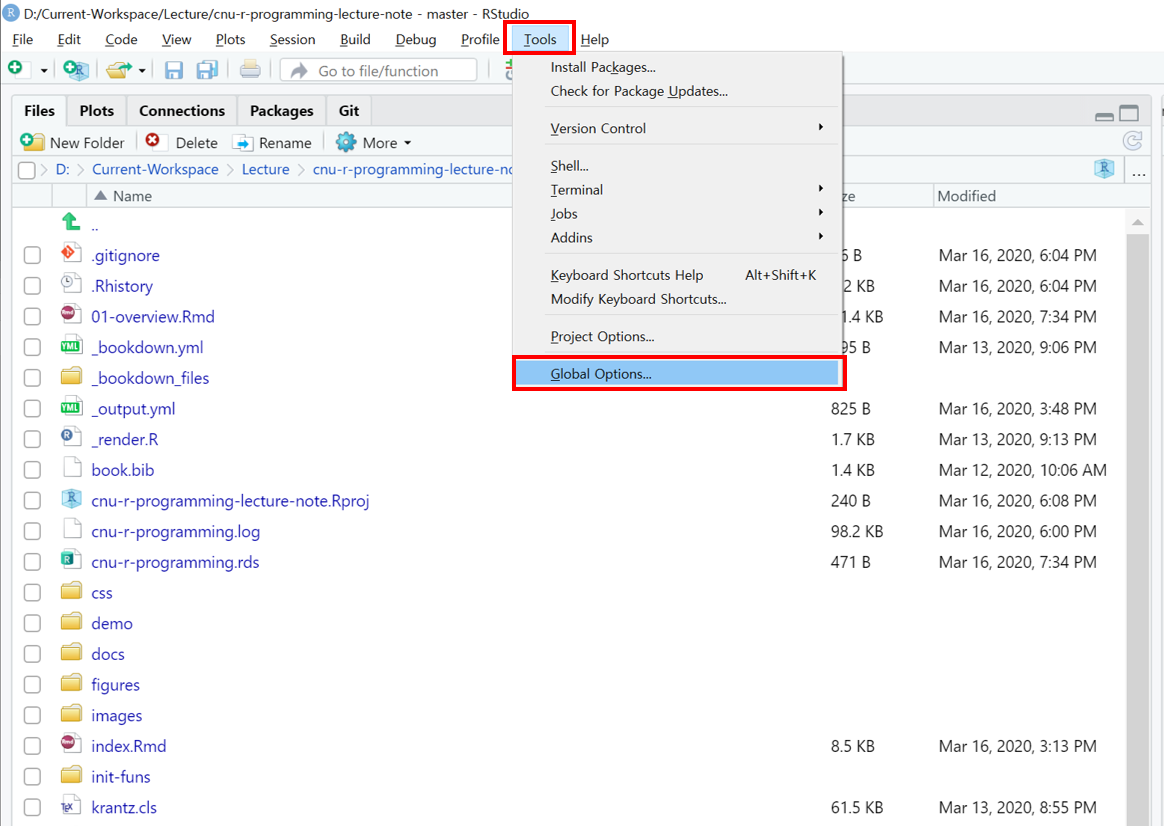
\includegraphics[width=0.8\linewidth]{figures/rstudio-glob-menu} \end{center}

\normalsize

\textbf{General}: RStudio 운용 관련 전반적 설정 세팅

\footnotesize

\begin{figure}

{\centering 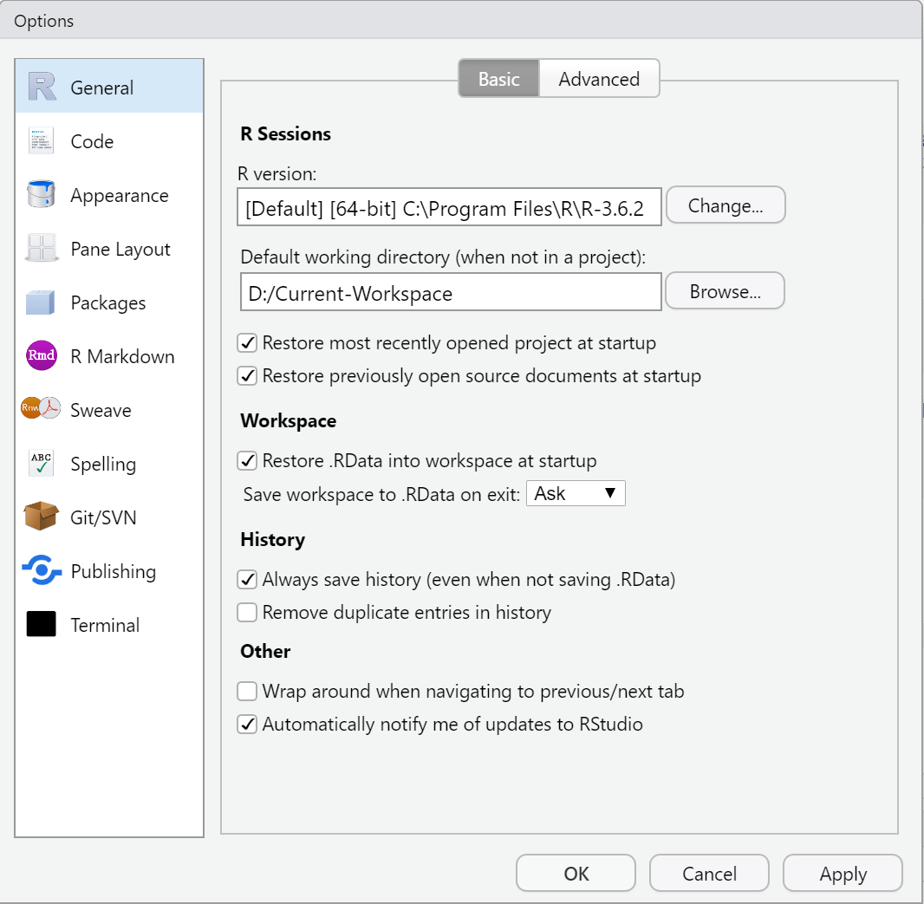
\includegraphics[width=0.8\linewidth]{figures/rstudio-glob-option} 

}

\caption{R General option 팝업 창}\label{fig:rstudio-glob-option}
\end{figure}

\normalsize

\begin{itemize}
\tightlist
\item
  \textbf{R version}: 만약 컴퓨터에 두 개 이상 다른 R 버전이 설치되어 있는 경우 \texttt{{[}Change{]}} 클릭 후 설정 변경 가능
\item
  \textbf{Default Working directory}: 작업 디렉토리 지정({[}\texttt{Browse}{]} 클릭 후 임의 폴더 설정 가능)
\item
  \textbf{Restore most recently opened project at startup}: RStudio 실행 시 가장 최근에 작업한 프로젝트로 이동
\item
  \textbf{Restore previously open source documents at startup}: RStudio 실행 시 현재 프로젝트에서 가장 최근에 작업한 소스코드 문서를 함께 열어줌.
\item
  \textbf{Restore .RData into workspace at startup}: 작업 디렉토리에 존재하는 \texttt{.RData} 파일을 RStudio 실행 시 불러옴
\item
  \textbf{Save workspace to .RData on exit}: R workspace 자동 저장(\texttt{.RData}) 여부
\item
  \textbf{Always save history (even when not saving .RData) }: R 실행 명령 history 저장 여부(Always/Never/Ask)
\item
  \textbf{Remove duplicate entries in history}: history 저장 시 중복 명령 제거 여부
\end{itemize}

작업폴더(Working Directory)는 현재 R session에서 사용하는 기본 폴더로서 R 소스파일 및 데이터의 저장 및 로딩시 기본이 되는 폴더임.

\begin{itemize}
\tightlist
\item
  소스파일이나 데이터를 불러들일 때 작업 폴더에 있는 파일은 경로명을 지정하지 않고 파일명만 사용해도 됨
\item
  작업폴더가 아닌 곳에 있는 파일을 불러들일 때는 경로명까지 써 주어야함.
\item
  R 데이터를 저장할때도 파일명만 쓰면 기본적으로 작업폴더에 저장되며, 다른 폴더에 저장하기 위해서는 경로명까지 써 주어야 함.
\end{itemize}

처음 컴퓨터에 RStudio를 설치하면 Working directory는 Windows 사용자 폴더(예: \texttt{user})의 \texttt{Document} 폴더가 기본값으로 설정되어 있음. 기본 작업폴더를 변경하려면 Figure \ref{fig:rstudio-glob-option}에서 설정 가능.

현재 R session의 작업 디렉토리 설정 방법

\begin{itemize}
\tightlist
\item
  \texttt{{[}Session{]}\ -\textgreater{}\ {[}Set\ Working\ Directoy{]}\ -\textgreater{}\ {[}Choose\ Directory{]}}에서 설정
\end{itemize}

\footnotesize

\begin{center}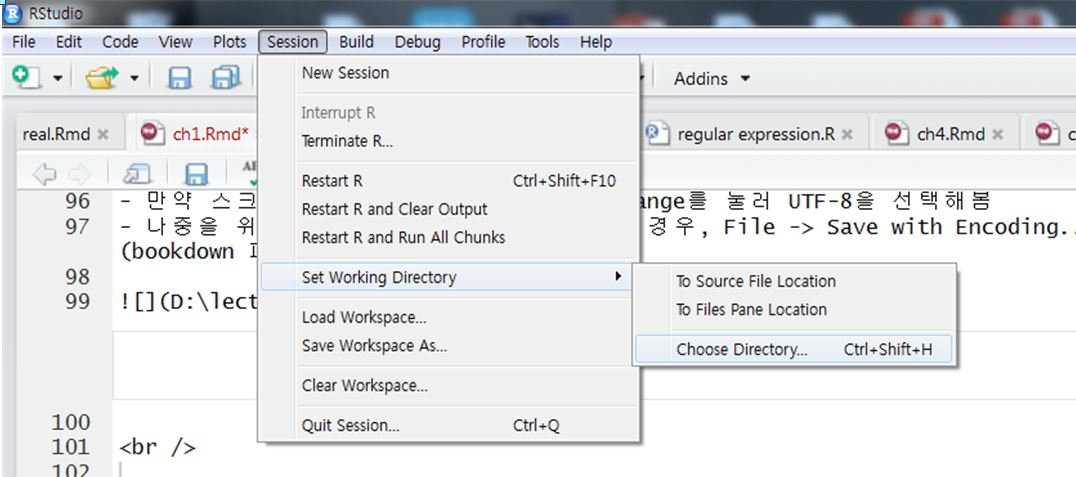
\includegraphics[width=0.8\linewidth]{figures/rstudio-wd-setting} \end{center}

\normalsize

R 콘솔에서 다음과 같은 명령어로 작업폴더를 확인 및 변경 가능

\footnotesize

\begin{Shaded}
\begin{Highlighting}[]
\KeywordTok{getwd}\NormalTok{() }\CommentTok{# 작업폴더 확인}
\end{Highlighting}
\end{Shaded}

\begin{verbatim}
[1] "D:/Current-Workspace/Lecture/cnu-r-programming-lecture-note"
\end{verbatim}

\normalsize

\footnotesize

\begin{Shaded}
\begin{Highlighting}[]
\KeywordTok{setwd}\NormalTok{(}\StringTok{".."}\NormalTok{) }\CommentTok{# 차상위 폴더로 이동}
\KeywordTok{getwd}\NormalTok{()}
\end{Highlighting}
\end{Shaded}

\begin{verbatim}
[1] "D:/Current-Workspace/Lecture"
\end{verbatim}

\begin{Shaded}
\begin{Highlighting}[]
\KeywordTok{setwd}\NormalTok{(}\StringTok{"../.."}\NormalTok{) }\CommentTok{# 차차상위 폴더로 이동}
\KeywordTok{getwd}\NormalTok{()}
\end{Highlighting}
\end{Shaded}

\begin{verbatim}
[1] "D:/"
\end{verbatim}

\begin{Shaded}
\begin{Highlighting}[]
\KeywordTok{setwd}\NormalTok{(}\StringTok{"D:/Current-Workspace/Lecture/misc/"}\NormalTok{) }\CommentTok{# 절대 폴더 명 입력}
\KeywordTok{setwd}\NormalTok{(}\StringTok{".."}\NormalTok{)}
\CommentTok{# dir() # 폴더 내 파일 명 출력}
\KeywordTok{getwd}\NormalTok{()}
\end{Highlighting}
\end{Shaded}

\begin{verbatim}
[1] "D:/Current-Workspace/Lecture"
\end{verbatim}

\begin{Shaded}
\begin{Highlighting}[]
\KeywordTok{setwd}\NormalTok{(}\StringTok{"misc"}\NormalTok{) }\CommentTok{# Current-Workspace 하위폴더인 misc 으로 이동}
\KeywordTok{getwd}\NormalTok{()}
\end{Highlighting}
\end{Shaded}

\begin{verbatim}
[1] "D:/Current-Workspace/Lecture/misc"
\end{verbatim}

\begin{Shaded}
\begin{Highlighting}[]
\KeywordTok{setwd}\NormalTok{(}\StringTok{"D:/Current-Workspace/Lecture/cnu-r-programming-lecture-note/"}\NormalTok{)}
\KeywordTok{getwd}\NormalTok{()}
\end{Highlighting}
\end{Shaded}

\begin{verbatim}
[1] "D:/Current-Workspace/Lecture/cnu-r-programming-lecture-note"
\end{verbatim}

\normalsize

\footnotesize

\BeginKnitrBlock{rmdcaution}
R에서 디렉토리 또는 폴더 구분자는 \texttt{/} 임. Windows에서 사용하는 구분자는 \texttt{\textbackslash{}}인데, R에서 \texttt{\textbackslash{}}는 특수문자로 간주하기 때문에 Windows 의 폴더명을 그대로 사용 시 에러 메세지를 출력함. 이를 해결하기 위해 Windows 경로명을 그대로 복사한 경우 경로 구분자 \texttt{\textbackslash{}} 대신 \texttt{\textbackslash{}\textbackslash{}}로 변경

\textbf{실습}: \texttt{C:\textbackslash{}r-project}를 컴퓨터에 생성 후 해당 폴더를 default 작업폴더로 설정
\EndKnitrBlock{rmdcaution}

\normalsize

\textbf{Code: Editing}: 들여쓰기, 자동 줄바꿈 등 코드 편집에 대한 전반적 설정

\footnotesize

\begin{center}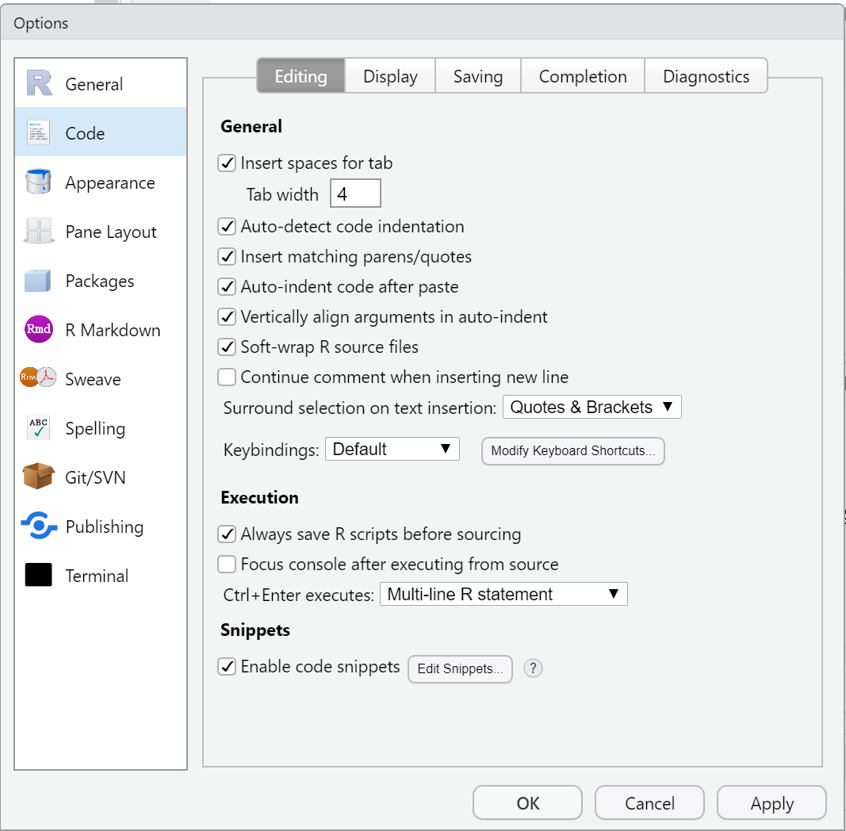
\includegraphics[width=0.8\linewidth]{figures/rstudio-code-edit-option} \end{center}

\normalsize

\begin{itemize}
\tightlist
\item
  \textbf{Insert spaces for tab}: \texttt{{[}Tab{]}} 키를 눌렀을 때 공백(space) 개수 결정(본 강의노트: \texttt{Tab\ width\ =\ 4})
\item
  \textbf{Auto-detect code indentation}: 코들 들여쓰기 자동 감지
\item
  \textbf{Insert matching parens/quotes}: 따옴표, 괄호 입력 시 커서를 따옴표/괄호 사이로 자동 이동
\item
  \textbf{Auto-indent code after paste}: 코드 복사 시 들여쓰기 일괄 적용
\item
  \textbf{Vertically align arguments in auto-indent}: 함수 작성 시 들여쓰기 레벨 유지 여부
\item
  \textbf{Soft-wrap R source file}: 스크립트 편집기 너비를 초과하는 경우 R 코드 행을 자동 줄바꿈
\item
  \textbf{Continue comment when inserting new line}: 주석 표시를 다음 행에도 자동 적용 여부
\item
  \textbf{Surround selection on text insertino}: 스크립트 상 text 선택 후 자동 따옴표 및 괄호 적용 여부
\item
  \textbf{Focus console after executing from source}: 스크립트 실행 후 커서 위치를 콘솔로 이동 여부
\end{itemize}

\textbf{Code: Display}: 스크립트(소스) 에디터 표시 화면 설정

\footnotesize

\begin{center}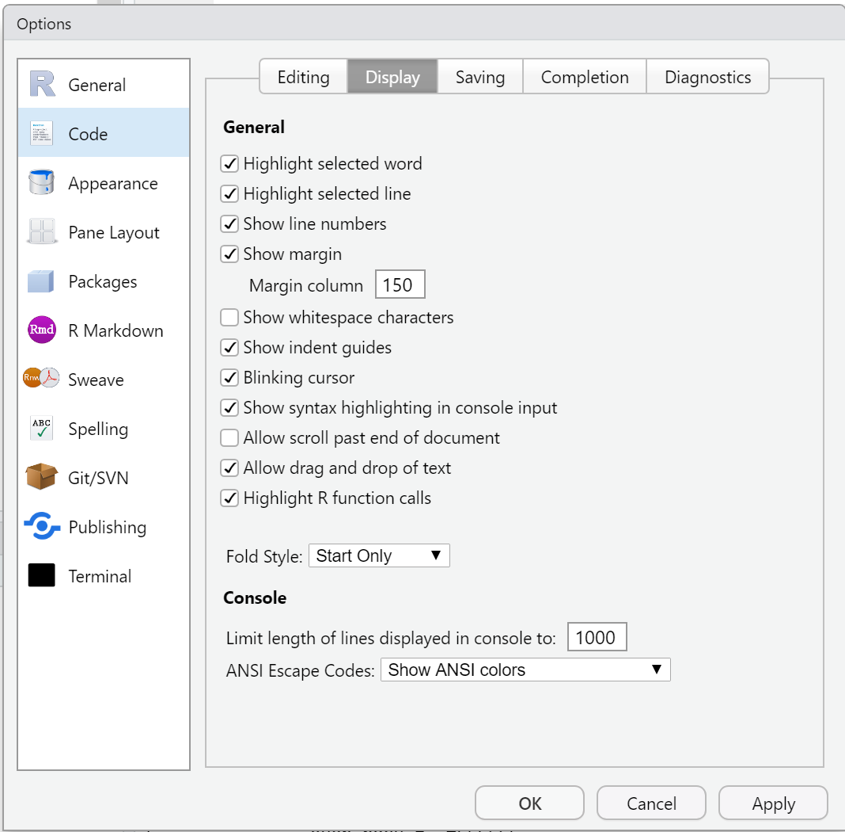
\includegraphics[width=0.8\linewidth]{figures/rstudio-code-display} \end{center}

\normalsize

\begin{itemize}
\tightlist
\item
  \textbf{Highlight selected word}: 스크립트 내 text 선택 시 동일한 text에 대해 배경강조 효과 여부
\item
  \textbf{Highlight selected line}: 선택된 행에 대해 배경 강조효과 여부
\item
  \textbf{Show line numbers}: 행 번호 보여주기 여부
\item
  \textbf{Show margin}: 소스 에디터 오른 쪽에 지정한 margin column 보여주기 여부
\item
  \textbf{Show whitespace characters}: 에디터에 공백 표시 여부
\item
  \textbf{Show indent guides}: 현재 들여쓰기 열 표시 여부
\item
  \textbf{Blinking cursor}: 커서 깜박임 여부
\item
  \textbf{Show syntax highlighting in console output}: 콘솔 입력 라인에 R 구문 강조 표시 적용 여부
\item
  \textbf{Allow scroll past end of document}: 문서 마지막 행 이후 스크롤 허용 여부
\item
  \textbf{Allow drag and drop of text}: 선택한 복수의 행으로 구성된 text에 대해 마우스 drag 허용
\item
  \textbf{Highlight R function calls}: R 내장 및 패키지 제공함수에 대해 강조 여부
\end{itemize}

\textbf{Code: Saving}: 스크립트(소스) 에디터 저장 설정

\footnotesize

\begin{center}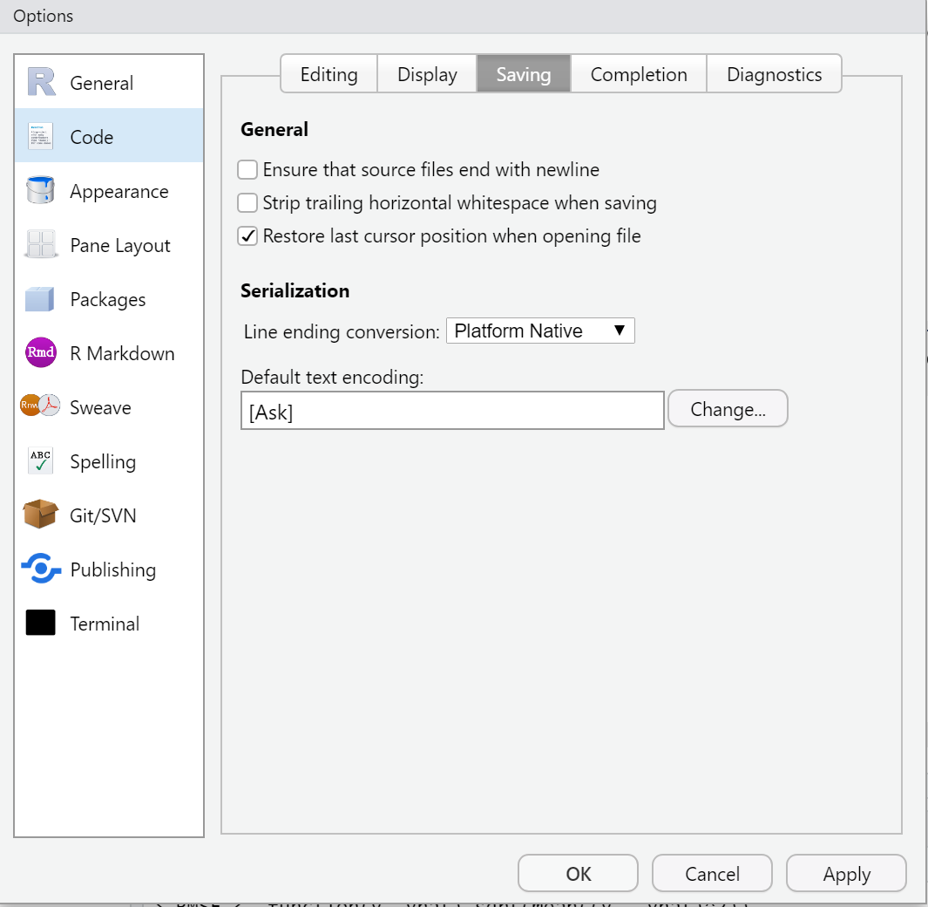
\includegraphics[width=0.8\linewidth]{figures/rstudio-code-saving} \end{center}

\normalsize

\begin{itemize}
\tightlist
\item
  \textbf{Ensure that source file end with newline}
\item
  \textbf{String trailing horizontal whitespace when saving}
\item
  \textbf{Restore last cursor position when opening file}
\item
  \textbf{Default text encoding}: 소스 에디터의 기본 설정 인코딩 설정 변경

  \begin{itemize}
  \tightlist
  \item
    RStudio의 Windows 버전 기본 text encoding은 \texttt{CP949} 임
  \item
    Linux나 Mac OS의 경우 한글은 \texttt{UTF-8}로 인코딩이 설정되어 있음.
  \item
    R 언어는 Linux 환경에서 개발되었기 때문에 \texttt{UTF-8} 인코딩과 호환성이 더 좋음
  \item
    스크립트 파일의 한글이 깨질 때는 \texttt{{[}File{]}\ -\textgreater{}\ {[}Reopen\ with\ Encoding...{]}}에서 encoding 방식 변경
  \end{itemize}
\end{itemize}

\textbf{Appearance}: RStudio 전체 폰트, 폰트 크기, theme 설정

\footnotesize

\begin{center}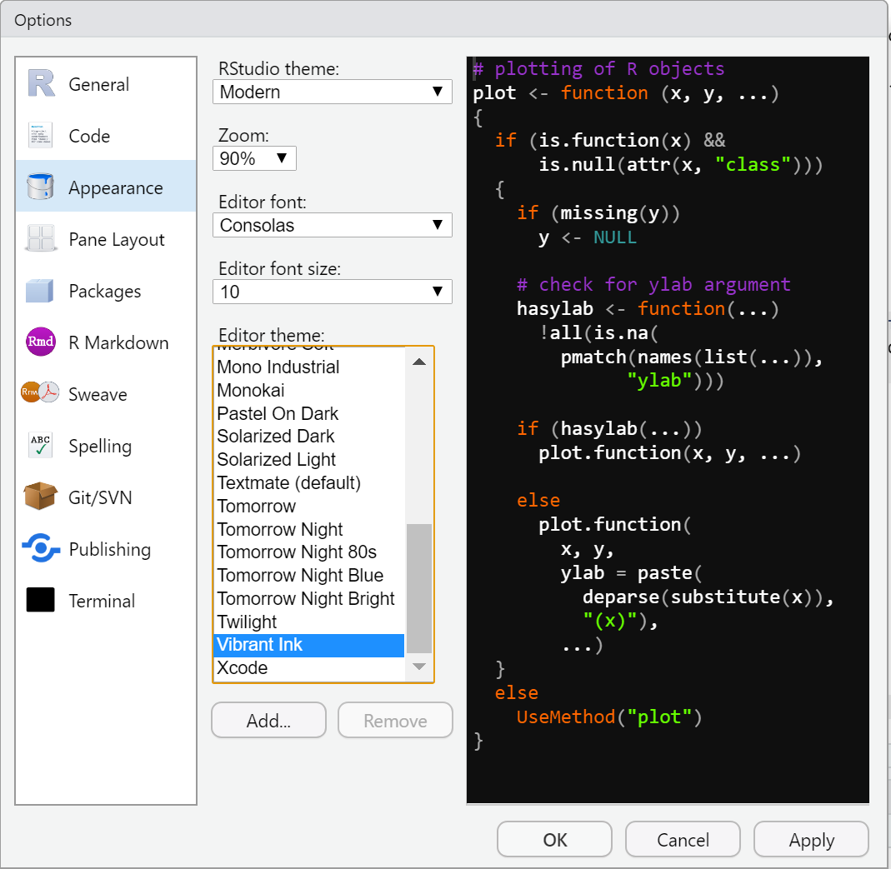
\includegraphics[width=0.8\linewidth]{figures/rstudio-appearance} \end{center}

\normalsize

\begin{itemize}
\tightlist
\item
  본인의 취향에 맞게 폰트 및 테마(theme) 설정
\item
  취향 \(\rightarrow\) 가독성이 제일 좋고 편안한 theme
\end{itemize}

\textbf{Pane Layout}: RStudio 구성 패널들의 위치 및 항목 등을 수정/추가/삭제(4개 페널은 항시 유지)

\footnotesize

\begin{center}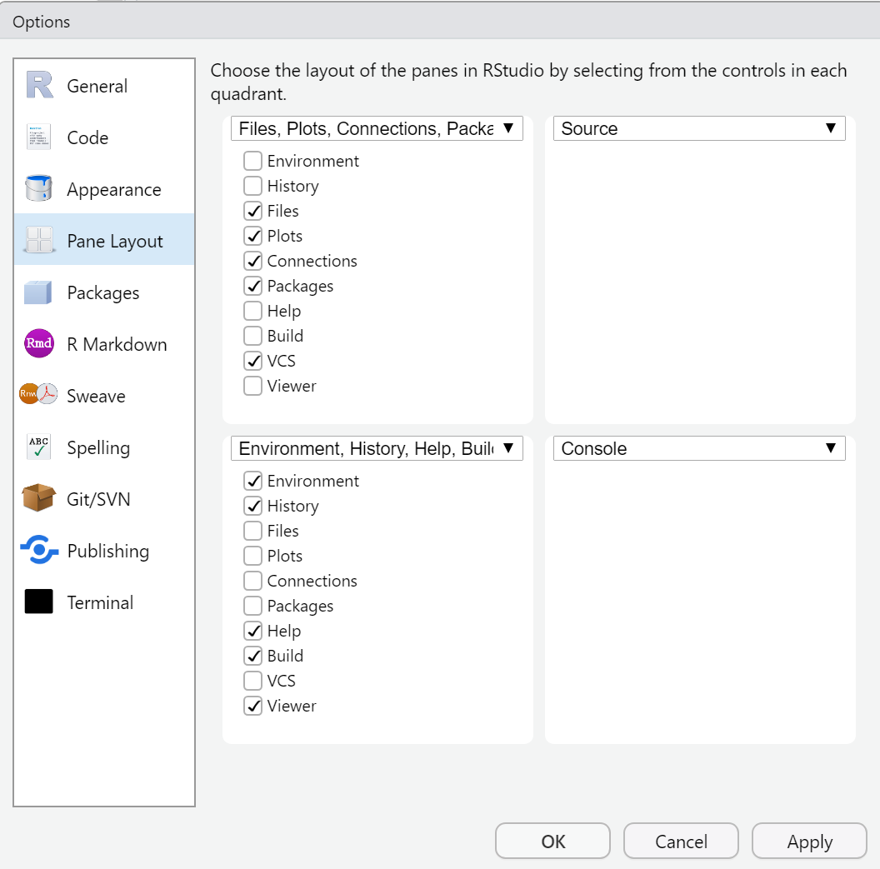
\includegraphics[width=0.8\linewidth]{figures/rstudio-pane-layout} \end{center}

\normalsize

\footnotesize

\BeginKnitrBlock{rmdimportant}
\textbf{실습}: 개인 취향에 맞게 RStudio 에디터 및 theme을 변경해 보자!!
\EndKnitrBlock{rmdimportant}

\normalsize

\hypertarget{rstudio-project}{%
\subsection{RStudio 프로젝트}\label{rstudio-project}}

\begin{enumerate}
\def\labelenumi{\arabic{enumi}.}
\tightlist
\item
  프로젝트

  \begin{itemize}
  \tightlist
  \item
    물리적 측면: 최종 산출물(문서)를 생성하기 위한 데이터, 사진, 그림 등을 모아 놓은 폴더
  \item
    논리적 측면: R session 및 작업의 버전 관리
  \end{itemize}
\item
  프로젝트의 필요성

  \begin{itemize}
  \tightlist
  \item
    자료의 정합성 보장
  \item
    다양한 확장자를 갖는 파일들이 한 폴더 내에 뒤섞일 때 곤란해 질 수 있음
  \item
    실제 분석 및 그래프 생성에 사용한 정확한 프로그램 또는 코드 연결이 어려움
  \end{itemize}
\item
  좋은 프로젝트 구성을 위한 방법

  \begin{itemize}
  \tightlist
  \item
    원자료(raw data)의 보호: 가급적 자료를 읽기 전용(read only) 형태로 다루기
  \item
    데이터 정제(data wrangling 또는 data munging)를 위한 스크립트와 정제 자료를 보관하는 읽기 전용 데이터 디렉토리 생성
  \item
    작성한 스크립트로 생성한 모든 산출물(테이블, 그래프 등)을 ``일회용품''처럼 처리 \(\rightarrow\) 스크립트로 재현 가능
  \item
    한 프로젝트 내 각기 다른 분석마다 다른 하위 디렉토리에 출력결과 저장하는 것이 유용
  \end{itemize}
\item
  RStudio 새로운 프로젝트 생성

  \begin{itemize}
  \tightlist
  \item
    RStudio의 강력하고 유용한 기능
  \item
    새로운 프로젝트 생성: RStudio 메뉴에서 \texttt{{[}File{]}} \(\rightarrow\) \texttt{{[}New\ Project{]}} 선택하면 아래와 같은 팝업 메뉴 생성
  \end{itemize}
\end{enumerate}

\footnotesize

\begin{center}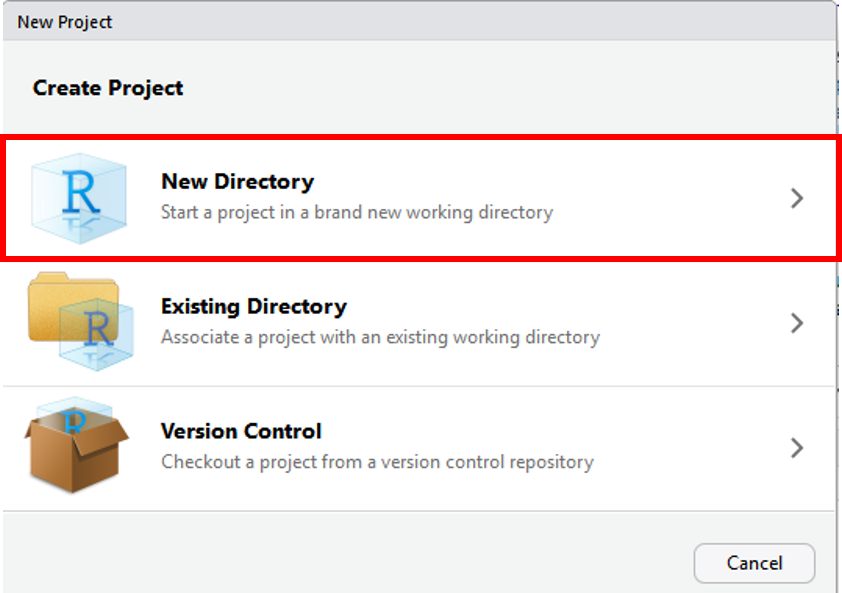
\includegraphics[width=0.8\linewidth]{figures/R-newproject-01} \end{center}

\normalsize

\begin{enumerate}
\def\labelenumi{\arabic{enumi}.}
\setcounter{enumi}{3}
\tightlist
\item
  위 그림에서 \texttt{New\ Directory}를 선택하면 아래와 같은 팝업 창이 나타나면 아래와 같은 프로젝트 유형이 나타남. 여기서는 \texttt{New\ Project} 선택
\end{enumerate}

\footnotesize

\begin{center}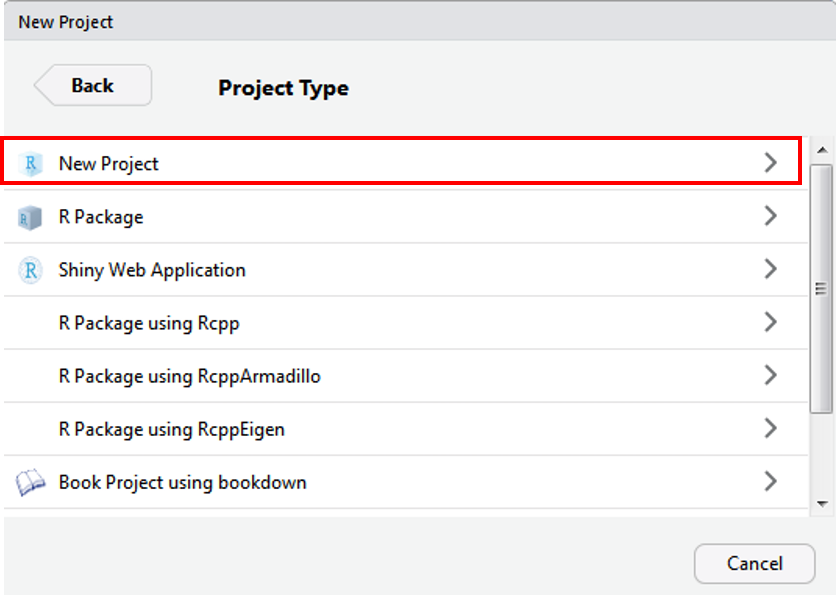
\includegraphics[width=0.8\linewidth]{figures/R-newproject-02} \end{center}

\normalsize

\begin{enumerate}
\def\labelenumi{\arabic{enumi}.}
\setcounter{enumi}{4}
\tightlist
\item
  다음 팝업창에서 새로운 프로젝트의 폴더명을 지정 후 \texttt{Create\ Project} 클릭

  \begin{itemize}
  \tightlist
  \item
    아래 \texttt{{[}Create\ projects\ as\ subdirectories\ of{]}}에서 생성하고자 하는 프로젝트의 상위 디렉토리 설정 \(\rightarrow\) 보통 RStudio의 기본 작업폴더로 설정
  \end{itemize}
\end{enumerate}

\footnotesize

\begin{center}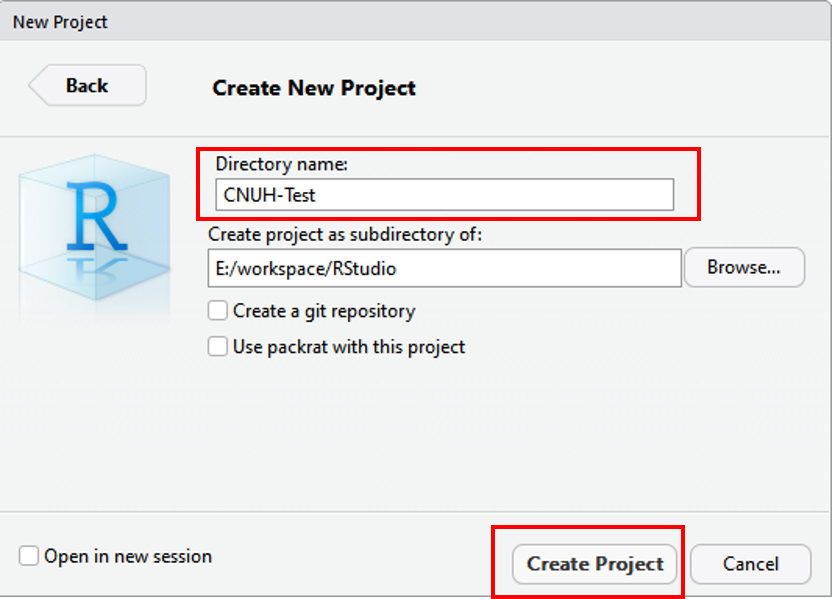
\includegraphics[width=0.8\linewidth]{figures/R-newproject-03} \end{center}

\normalsize

\begin{enumerate}
\def\labelenumi{\arabic{enumi}.}
\setcounter{enumi}{5}
\tightlist
\item
  현재 R session 종료 후 새로운 프로젝트로 session 화면이 열리면 프로젝트 생성 완료
\end{enumerate}

\footnotesize

\BeginKnitrBlock{rmdimportant}
\textbf{실습}: 프로젝트 생성

\begin{itemize}
\tightlist
\item
  위에서 설정한 작업폴더 내에 \texttt{학번-r-programming} 프로젝트 생성
\item
  생성한 프로젝트 폴더 내에 \texttt{docs}, \texttt{figures}, \texttt{script} 폴더 생성
\end{itemize}
\EndKnitrBlock{rmdimportant}

\normalsize

\hypertarget{r-package}{%
\section{R 패키지}\label{r-package}}

\footnotesize

\BeginKnitrBlock{rmdnote}
\textbf{R 패키지(package)}: 특수 목적을 위한 로직으로 구성된 코드들의 집합으로 R에서 구동되는 분석툴을 통칭

\begin{itemize}
\tightlist
\item
  CRAN을 통해 배포: 3자가 이용하기 쉬움 \(\rightarrow\) R 시스템 환경에서 패키지는 가장 중요한 역할
\item
  CRAN \href{https://cran.r-project.org/web/packages/available_packages_by_date.html}{available package by name} 또는 \href{https://cran.r-project.org/web/packages/available_packages_by_name.html}{available package by date}에서 현재 등재된 패키지 리스트 확인 가능
\item
  R console에서 \texttt{available.packages()} 함수를 통해서도 확인 가능
\item
  현재 CRAN 기준(2020-03-17) 배포된 패키지의 개수는 16045 개임
\end{itemize}

\textbf{목적}: RStudio 환경에서 패키지를 설치하고 불러오기
\EndKnitrBlock{rmdnote}

\normalsize

\hypertarget{r-package-path}{%
\subsection{R 패키지 경로 확인 및 변경}\label{r-package-path}}

\begin{itemize}
\tightlist
\item
  패키지 설치 시 일반적으로 R 환경에서 기본값으로 지정한 라이브러리 폴더에 저장
\item
  패키지 설치 전 R 패키지 설치 경로(path) 지정
\item
  \texttt{.libPaths()} 함수를 통해 현재 설정된 패키지 저장 경로 확인
\end{itemize}

\footnotesize

\begin{Shaded}
\begin{Highlighting}[]
\KeywordTok{.libPaths}\NormalTok{()}
\end{Highlighting}
\end{Shaded}

\begin{verbatim}
[1] "C:/Users/user/Documents/R/win-library/3.6"
[2] "C:/Program Files/R/R-3.6.3/library"       
\end{verbatim}

\normalsize

\begin{itemize}
\tightlist
\item
  일반적으로 첫 번째 경로를 디폴트 라이브러리 폴더로 사용
\item
  사용자 지정 라이브러리 경로를 설정 하려면 아래와 같은 절차로 진행
\end{itemize}

\begin{quote}
\textbf{실습: c:/r-library 폴더를 패키지 경로로 지정}
\end{quote}

\begin{enumerate}
\def\labelenumi{\arabic{enumi})}
\item
  \texttt{C:\textbackslash{}}에서 {[}새로 만들기(W){]} -\textgreater{} {[}폴더(F){]} 선택 후 생성 폴더 이름을 \texttt{r-library}로 변경
\item
  윈도우즈 \texttt{{[}제어판{]}\ -\textgreater{}\ {[}시스템\ 및\ 보안{]}\ -\textgreater{}\ {[}시스템{]}\ -\textgreater{}\ {[}고급\ 시스템\ 설정{]}} 클릭
\end{enumerate}

\footnotesize

\begin{center}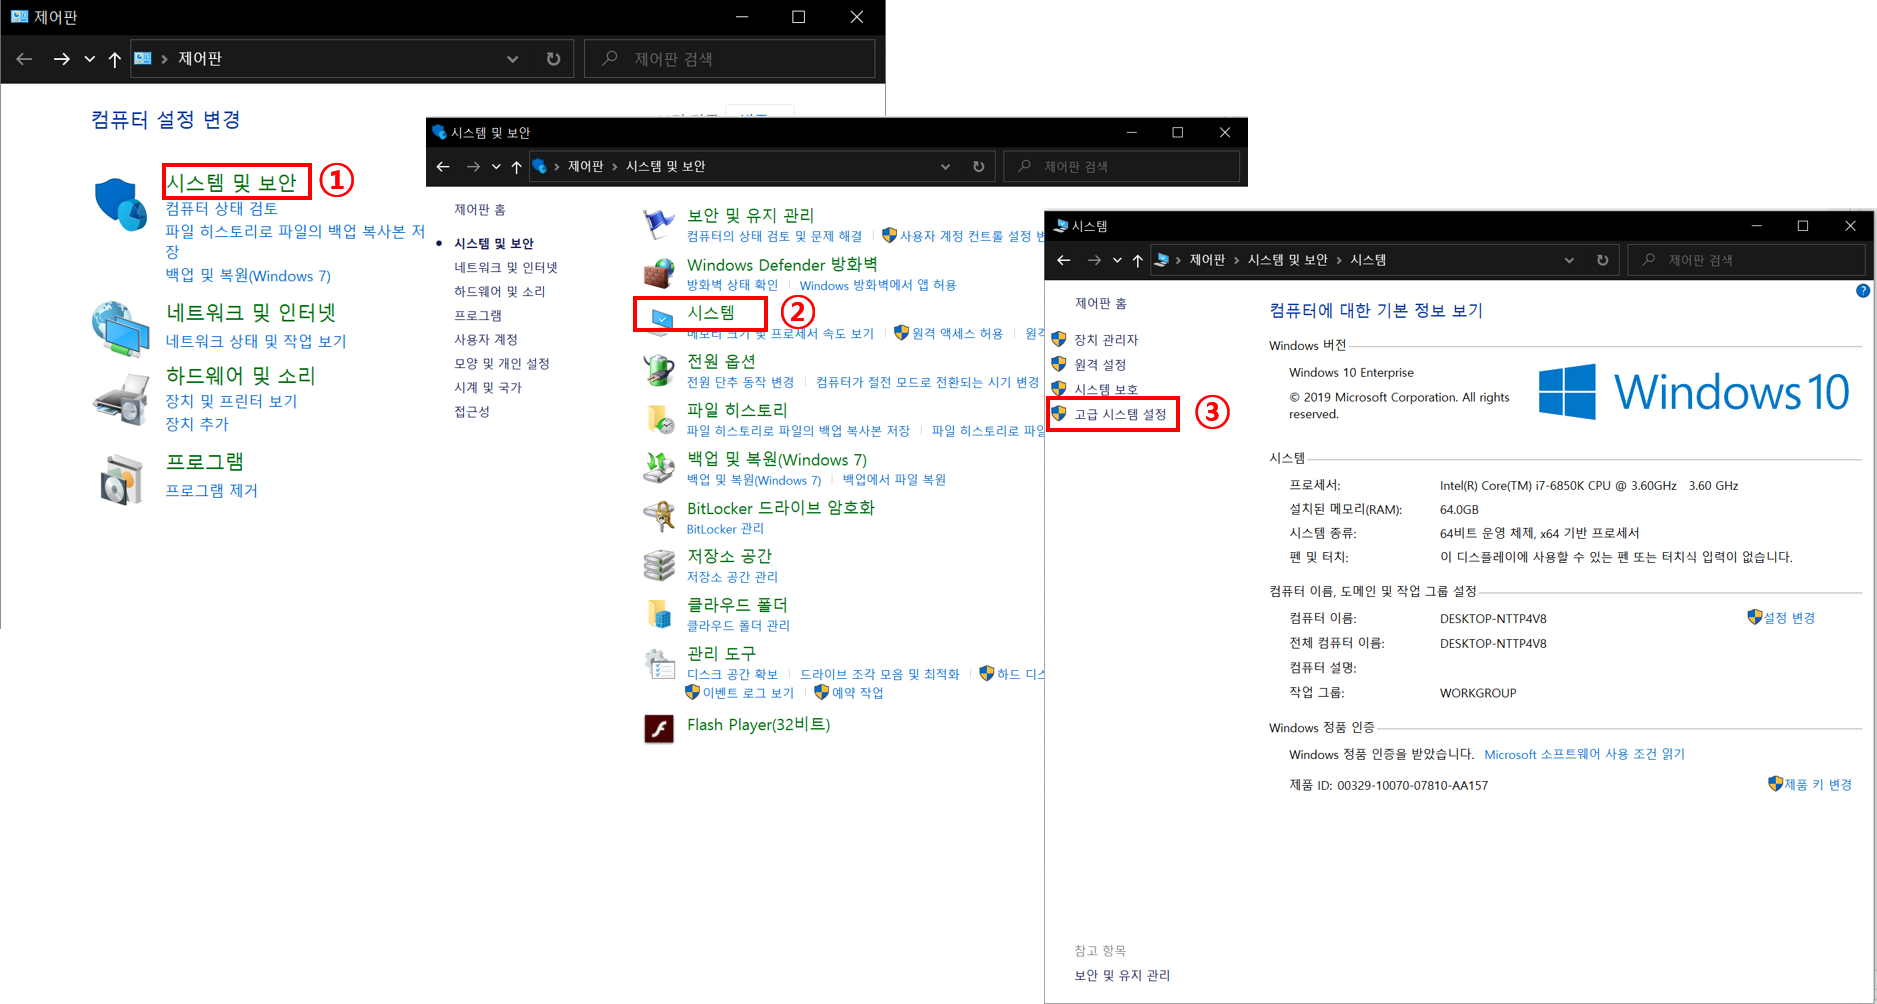
\includegraphics[width=0.8\linewidth]{figures/window-env-system} \end{center}

\normalsize

\begin{enumerate}
\def\labelenumi{\arabic{enumi})}
\setcounter{enumi}{2}
\tightlist
\item
  \texttt{{[}환경변수(N)...{]}} 선택 후 시스템 변수에서 \texttt{{[}새로\ 만들기(W)...{]}} 클릭
\end{enumerate}

\footnotesize

\begin{center}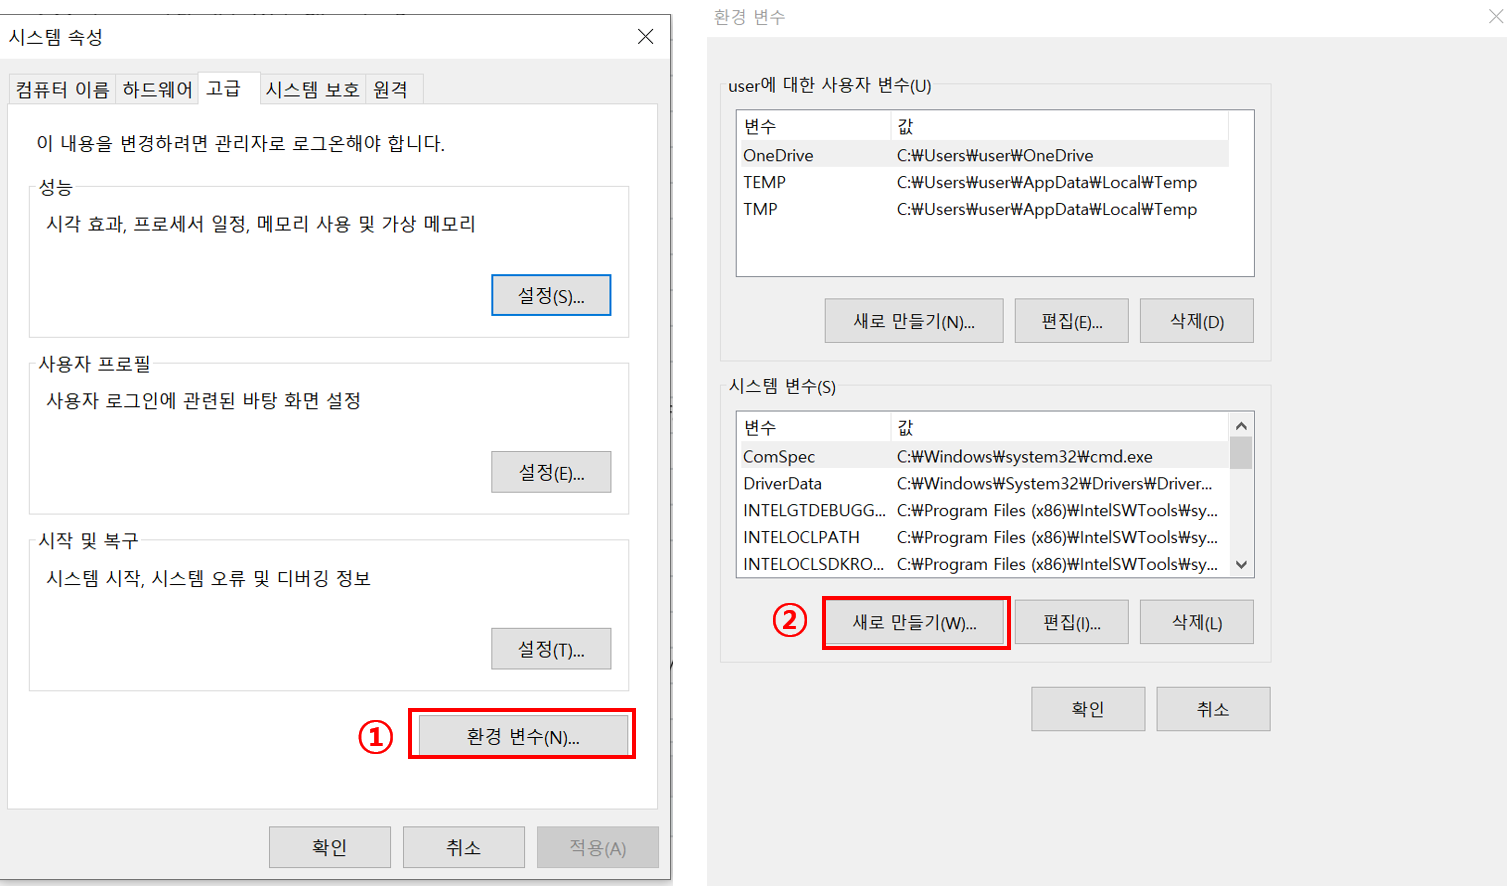
\includegraphics[width=0.8\linewidth]{figures/window-env-var} \end{center}

\normalsize

\begin{enumerate}
\def\labelenumi{\arabic{enumi})}
\setcounter{enumi}{3}
\tightlist
\item
  아래 그림과 같이 변수 이름(N)에 \texttt{R\_LIBS}, 변수 값(V)에 해당 디렉토리 경로 \texttt{C:\textbackslash{}r-library} 입력 후 확인 버튼 클릭
\end{enumerate}

\footnotesize

\begin{center}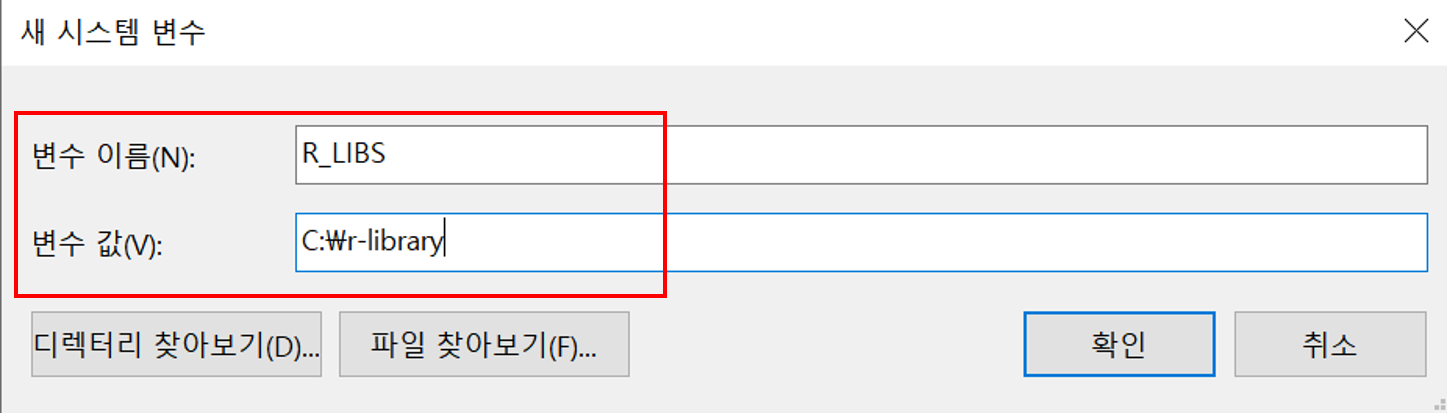
\includegraphics[width=0.9\linewidth]{figures/window-new-system-var} \end{center}

\normalsize

\begin{enumerate}
\def\labelenumi{\arabic{enumi})}
\setcounter{enumi}{4}
\tightlist
\item
  현재 RStudio 종료 후 재실행한 다음 콘솔창에 \texttt{.libPaths()} 입력 후 라이브러리 경로 확인
\end{enumerate}

\hypertarget{r-package-install}{%
\subsection{R 패키지 설치하기}\label{r-package-install}}

\begin{itemize}
\tightlist
\item
  RStudio 메뉴 \texttt{{[}Tools{]}} \(\rightarrow\) \texttt{{[}Install\ packages{]}} 클릭 후 생성된 팝업 창에서 설치하고자 하는 패키지 입력 후 설치
\end{itemize}

\footnotesize

\begin{center}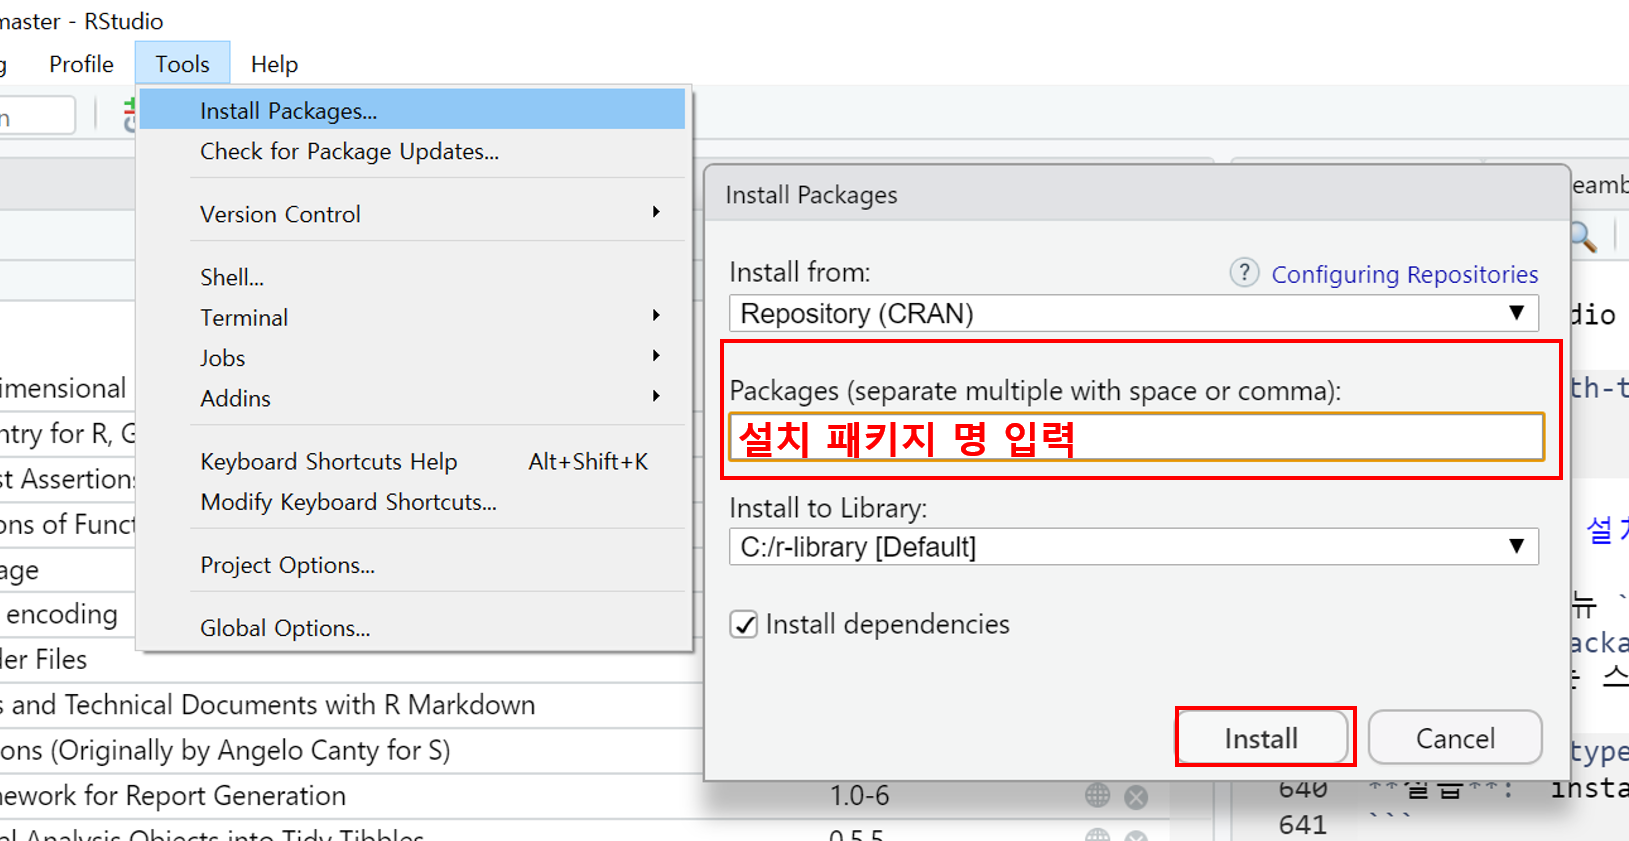
\includegraphics[width=0.8\linewidth]{figures/rstudio-package-install} \end{center}

\normalsize

\begin{itemize}
\tightlist
\item
  RStudio \texttt{Packages} 창에서 \texttt{{[}Install{]}} 버튼 누르면 위와 동일한 팝업창이 나타남(위와 동일)
\end{itemize}

\footnotesize

\begin{center}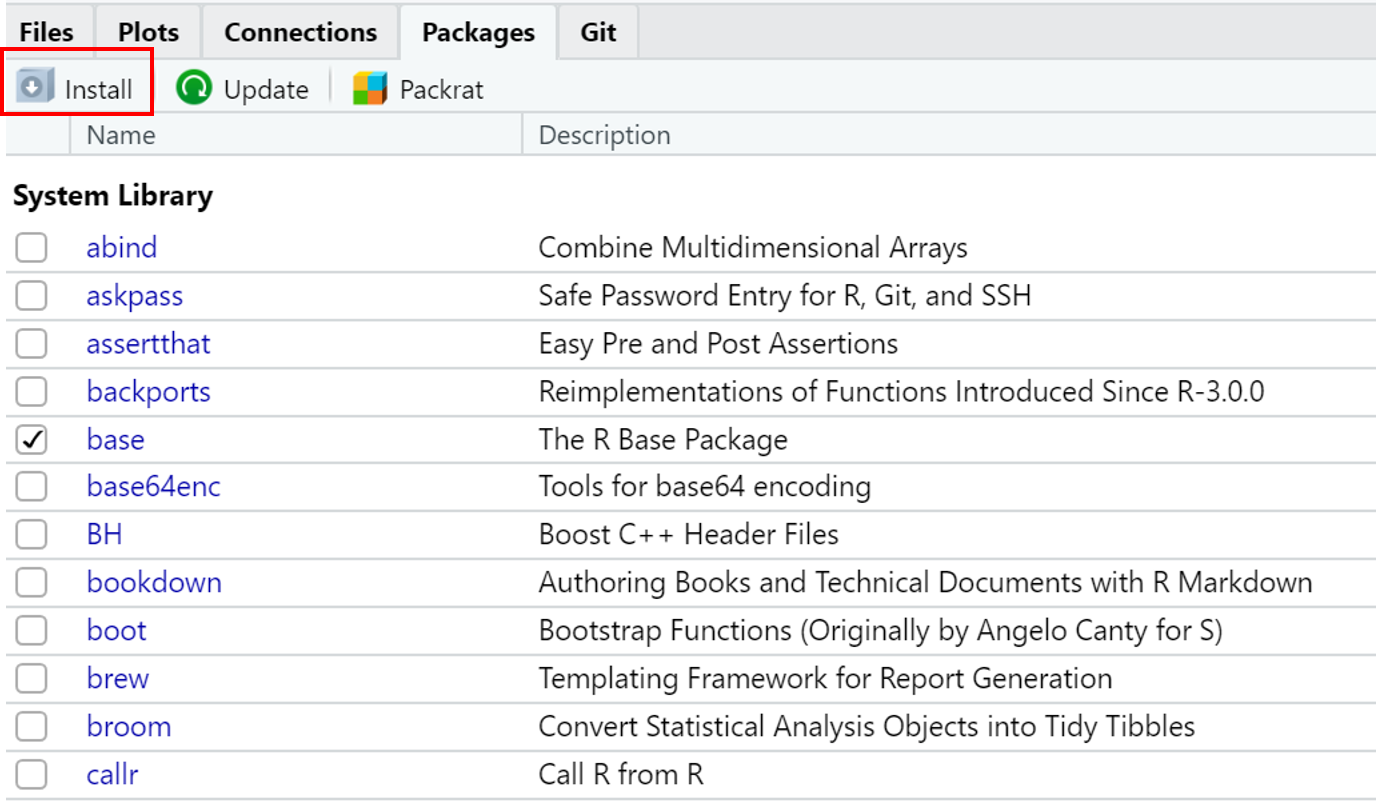
\includegraphics[width=0.8\linewidth]{figures/rstudio-pack-win-02} \end{center}

\normalsize

\begin{itemize}
\tightlist
\item
  R 콘솔 또는 스크립트 창에서 \texttt{install.packages(package\_name)} 함수를 사용해서 패키지 설치
\end{itemize}

\footnotesize

\BeginKnitrBlock{rmdimportant}
\textbf{실습}: \texttt{install.packages()} 함수를 이용해 \texttt{tidyverse} 패키지 설치
\EndKnitrBlock{rmdimportant}

\normalsize

\footnotesize

\begin{Shaded}
\begin{Highlighting}[]
\KeywordTok{install.packages}\NormalTok{(}\StringTok{"tidyverse"}\NormalTok{)}
\end{Highlighting}
\end{Shaded}

\normalsize

\begin{quote}
위 명령어를 실행하면 \texttt{tidyverse} 패키지 뿐 아니라 연관된 패키지들이 동시에 설치됨
\end{quote}

\hypertarget{r-package-load}{%
\subsection{R 패키지 불러오기}\label{r-package-load}}

\begin{enumerate}
\def\labelenumi{\arabic{enumi}.}
\tightlist
\item
  \texttt{library()} vs.~\texttt{require()}

  \begin{itemize}
  \tightlist
  \item
    \texttt{library()}: 불러오고자 하는 패키지가 시스템에 존재하지 않는 경우 에러 메세지 출력(에러 이후 명령어들이 실행되지 않음)
  \item
    \texttt{require()}: 패키지가 시스템에 존재하지 않는 경우 경고 메세지 출력(경고 이후 명령어 정상적으로 실행)
  \end{itemize}
\item
  다중 패키지 동시에 불러오기

  \begin{itemize}
  \tightlist
  \item
    RStudio \texttt{Packages} 창에서 설치하고자 하는 패키지 선택 버튼 클릭하면 R workspace로 해당 패키지 로드 가능
  \item
    스크립트 이용
  \end{itemize}
\end{enumerate}

\footnotesize

\BeginKnitrBlock{rmdimportant}
\textbf{실습}: \texttt{tidyverse} 패키지 불러오기
\EndKnitrBlock{rmdimportant}

\normalsize

\footnotesize

\begin{Shaded}
\begin{Highlighting}[]
\KeywordTok{require}\NormalTok{(tidyverse)}
\end{Highlighting}
\end{Shaded}

\begin{verbatim}
필요한 패키지를 로딩중입니다: tidyverse
\end{verbatim}

\begin{verbatim}
-- Attaching packages --------------------------------------------------------------------- tidyverse 1.3.0 --
\end{verbatim}

\begin{verbatim}
v ggplot2 3.3.0     v purrr   0.3.3
v tibble  2.1.3     v dplyr   0.8.5
v tidyr   1.0.2     v stringr 1.4.0
v readr   1.3.1     v forcats 0.5.0
\end{verbatim}

\begin{verbatim}
-- Conflicts ------------------------------------------------------------------------ tidyverse_conflicts() --
x dplyr::filter()     masks stats::filter()
x dplyr::group_rows() masks kableExtra::group_rows()
x dplyr::lag()        masks stats::lag()
\end{verbatim}

\normalsize

\footnotesize

\BeginKnitrBlock{rmdnote}
실무에서 R의 활용능력은 패키지 활용 여부에 달려 있음. 즉, 목적에 맞는 업무를 수행하기 위해 가장 적합한 패키지를 찾고 활용하느냐에 따라 R 활용능력의 차이를 보임. 앞서 언급한 바와 같이 CRAN에 등록된 패키지는 16000 개가 넘지만, 이 중 많이 활용되고 있는 패키지의 수는 약 200 \textasciitilde{} 300 개 내외이고, 실제 데이터 분석 시 10 \textasciitilde{} 20개 정도의 패키지가 사용됨. 앞 예제에서 설치하고 불러온 \texttt{tidyverse} 패키지는 Hadley Wickham \citep{tidyverse2019}이 개발한 데이터 전처리 및 시각화 패키지 번들이고, 현재 R 프로그램 환경에 지대한 영향을 미침. 본 강의 ``데이터프레임 가공 및 시각화''에서 해당 패키지 활용 방법을 배울 예정
\EndKnitrBlock{rmdnote}

\normalsize

\hypertarget{r-basic}{%
\section{R 기초 문법}\label{r-basic}}

\footnotesize

\BeginKnitrBlock{rmdnote}
본 절에서 다루는 R 문법은 R 입문 시 객체(object)의 명명 규칙과 R 콘솔 창에서 가장 빈번하게 사용되는 기초적인 명령어만 다룰 예정임. 심화 내용은 2-3주 차에 다룰 예정임.
\EndKnitrBlock{rmdnote}

\normalsize

\begin{itemize}
\tightlist
\item
  R은 객체지향언어(object-oriented language)

  \begin{itemize}
  \tightlist
  \item
    객체(object): 숫자, 데이터셋, 단어, 테이블, 분석결과 등 모든 것을 칭함
  \item
    ``객체지향''의 의미는 R의 모든 명령어는 객체를 대상으로 이루어진다는 것을 의미
  \end{itemize}
\end{itemize}

\footnotesize

\BeginKnitrBlock{rmdtip}
알아두면 유용한(콘솔창에서 매우 많이 사용되는) 명령어 및 단축키

\begin{itemize}
\tightlist
\item
  \texttt{ls()}: 현재 R 작업공간에 저장된 모든 객체 리스트 출력
\item
  \texttt{rm(object\_name)}: \texttt{object\_name}에 해당하는 객체 삭제
\item
  \texttt{rm(list\ =\ ls())}: R 작업공간에 저장된 모든 객체들을 일괄 삭제
\item
  단축키 \texttt{{[}Ctrl{]}\ +\ {[}L{]}}: R 콘솔 창 일괄 청소
\item
  단축키 \texttt{{[}Ctrl{]}\ +\ {[}Shift{]}\ +\ {[}F10{]}}: R session 초기화
\end{itemize}

\textbf{예시}
\EndKnitrBlock{rmdtip}

\normalsize

\footnotesize

\begin{Shaded}
\begin{Highlighting}[]
\NormalTok{x <-}\StringTok{ }\DecValTok{7}
\NormalTok{y <-}\StringTok{ }\DecValTok{1}\OperatorTok{:}\DecValTok{30} \CommentTok{#1에서 30까지 정수 입력}
\KeywordTok{ls}\NormalTok{() }\CommentTok{#현재 작업공간 내 객체명 출력}
\end{Highlighting}
\end{Shaded}

\begin{verbatim}
 [1] "a"                  "b"                  "cars"              
 [4] "def.chunk.hook"     "fig_cap"            "hook_output"       
 [7] "tab"                "x"                  "y"                 
[10] "도움말 보기 명령어" "사용법"             "설명"              
\end{verbatim}

\normalsize

\footnotesize

\begin{Shaded}
\begin{Highlighting}[]
\KeywordTok{rm}\NormalTok{(x) }\CommentTok{# 객체 x 삭제}
\KeywordTok{ls}\NormalTok{()}
\end{Highlighting}
\end{Shaded}

\begin{verbatim}
 [1] "a"                  "b"                  "cars"              
 [4] "def.chunk.hook"     "fig_cap"            "hook_output"       
 [7] "tab"                "y"                  "도움말 보기 명령어"
[10] "사용법"             "설명"              
\end{verbatim}

\begin{Shaded}
\begin{Highlighting}[]
\KeywordTok{rm}\NormalTok{(a,b) }\CommentTok{# 객체 a,b 동시 삭제}
\KeywordTok{ls}\NormalTok{()}
\end{Highlighting}
\end{Shaded}

\begin{verbatim}
[1] "cars"               "def.chunk.hook"     "fig_cap"           
[4] "hook_output"        "tab"                "y"                 
[7] "도움말 보기 명령어" "사용법"             "설명"              
\end{verbatim}

\begin{Shaded}
\begin{Highlighting}[]
\CommentTok{# rm(list = ls()) # 모든 객체 삭제}
\end{Highlighting}
\end{Shaded}

\normalsize

\hypertarget{r-object-nam-rule}{%
\subsubsection*{R 객체 입력 방법 및 변수 설정 규칙}\label{r-object-nam-rule}}


객체를 할당하는 두 가지 방법:\texttt{=}, \texttt{\textless{}-}

\begin{itemize}
\tightlist
\item
  두 할당 지시자의 차이점

  \begin{itemize}
  \tightlist
  \item
    \texttt{=}: 명령의 최상 수준에서만 사용 가능
  \item
    \texttt{\textless{}-}: 어디서든 사용 가능
  \item
    함수 호출과 동시에 변수에 값을 할당할 목적으로는 \texttt{\textless{}-}만 사용 가능
  \end{itemize}
\end{itemize}

\footnotesize

\begin{Shaded}
\begin{Highlighting}[]
\CommentTok{# mean(): 입력 벡터의 평균 계산}
\KeywordTok{mean}\NormalTok{(y <-}\StringTok{ }\DecValTok{1}\OperatorTok{:}\DecValTok{5}\NormalTok{)}
\end{Highlighting}
\end{Shaded}

\begin{verbatim}
[1] 3
\end{verbatim}

\begin{Shaded}
\begin{Highlighting}[]
\NormalTok{y}
\end{Highlighting}
\end{Shaded}

\begin{verbatim}
[1] 1 2 3 4 5
\end{verbatim}

\begin{Shaded}
\begin{Highlighting}[]
\KeywordTok{mean}\NormalTok{(}\DataTypeTok{x =} \DecValTok{1}\OperatorTok{:}\DecValTok{5}\NormalTok{)}
\end{Highlighting}
\end{Shaded}

\begin{verbatim}
[1] 3
\end{verbatim}

\begin{Shaded}
\begin{Highlighting}[]
\NormalTok{x}
\end{Highlighting}
\end{Shaded}

\begin{verbatim}
Error in eval(expr, envir, enclos): 객체 'x'를 찾을 수 없습니다
\end{verbatim}

\normalsize

객체 또는 변수의 명명 규칙

\begin{itemize}
\tightlist
\item
  알파벳, 한글, 숫자, \texttt{\_}, \texttt{.}의 조합으로 구성 가능(\texttt{-}은 사용 불가)
\item
  변수명의 알파벳, 한글, \texttt{.}로 시작 가능
\item
  \texttt{.}로 시작한 경우 뒤에 숫자 올 수 없음(숫자로 인지)
\item
  대소문자 구분
\end{itemize}

\footnotesize

\begin{Shaded}
\begin{Highlighting}[]
\CommentTok{# 1:10은 1부터 10까지 정수 생성}
\CommentTok{# 'c()'는 벡터 생성 함수}
\NormalTok{x <-}\StringTok{ }\KeywordTok{c}\NormalTok{(}\DecValTok{1}\OperatorTok{:}\DecValTok{10}\NormalTok{) }
\CommentTok{# 1:10으로 구성된 행렬 생성}
\NormalTok{X <-}\StringTok{ }\KeywordTok{matrix}\NormalTok{(}\KeywordTok{c}\NormalTok{(}\DecValTok{1}\OperatorTok{:}\DecValTok{10}\NormalTok{), }\DataTypeTok{nrow =} \DecValTok{2}\NormalTok{, }\DataTypeTok{ncol =} \DecValTok{5}\NormalTok{, }\DataTypeTok{byrow =}\NormalTok{ T)}
\NormalTok{x}
\end{Highlighting}
\end{Shaded}

\begin{verbatim}
 [1]  1  2  3  4  5  6  7  8  9 10
\end{verbatim}

\begin{Shaded}
\begin{Highlighting}[]
\NormalTok{X}
\end{Highlighting}
\end{Shaded}

\begin{verbatim}
     [,1] [,2] [,3] [,4] [,5]
[1,]    1    2    3    4    5
[2,]    6    7    8    9   10
\end{verbatim}

\begin{Shaded}
\begin{Highlighting}[]
\CommentTok{# 논리형 객체}
\NormalTok{.x <-}\StringTok{ }\OtherTok{TRUE}
\NormalTok{.x}
\end{Highlighting}
\end{Shaded}

\begin{verbatim}
[1] TRUE
\end{verbatim}

\begin{Shaded}
\begin{Highlighting}[]
\CommentTok{# 알파벳 + 숫자}
\CommentTok{# seq(): 수열을 만드는 함수}
\CommentTok{# 1 에서부터(from) 10 까지(to) 공차가 2(by)인 수열}
\NormalTok{a1 <-}\StringTok{ }\KeywordTok{seq}\NormalTok{(}\DataTypeTok{from =} \DecValTok{1}\NormalTok{, }\DataTypeTok{to =} \DecValTok{10}\NormalTok{, }\DataTypeTok{by =} \DecValTok{2}\NormalTok{)}
\CommentTok{# 한글 변수명}
\NormalTok{가수 <-}\StringTok{ }\KeywordTok{c}\NormalTok{(}\StringTok{"Damian Rice"}\NormalTok{, }\StringTok{"Beatles"}\NormalTok{, }\StringTok{"최백호"}\NormalTok{, }\StringTok{"Queen"}\NormalTok{, }\StringTok{"Carlos Gardel"}\NormalTok{, }\StringTok{"BTS"}\NormalTok{, }\StringTok{"조용필"}\NormalTok{)}
\NormalTok{가수}
\end{Highlighting}
\end{Shaded}

\begin{verbatim}
[1] "Damian Rice" "Beatles" "최백호"
"Queen"
[5] "Carlos Gardel" "BTS" "조용필"
\end{verbatim}

\normalsize

\begin{enumerate}
\def\labelenumi{\arabic{enumi}.}
\setcounter{enumi}{2}
\tightlist
\item
  잘못된 객체 또는 변수 명명 예시
\end{enumerate}

\footnotesize

\begin{Shaded}
\begin{Highlighting}[]
\NormalTok{3x <-}\StringTok{ }\DecValTok{7}
\end{Highlighting}
\end{Shaded}

\begin{verbatim}
Error: <text>:1:2: 예상하지 못한 기호(symbol)입니다.
1: 3x
     ^
\end{verbatim}

\normalsize

\footnotesize

\begin{Shaded}
\begin{Highlighting}[]
\NormalTok{_x <-}\StringTok{ }\KeywordTok{c}\NormalTok{(}\StringTok{"M"}\NormalTok{, }\StringTok{"M"}\NormalTok{, }\StringTok{"F"}\NormalTok{)}
\end{Highlighting}
\end{Shaded}

\begin{verbatim}
Error: <text>:1:1: 예상하지 못한 입력입니다.
1: _
    ^
\end{verbatim}

\normalsize

\footnotesize

\begin{Shaded}
\begin{Highlighting}[]
\FloatTok{.3}\NormalTok{ <-}\StringTok{ }\DecValTok{10}
\end{Highlighting}
\end{Shaded}

\begin{verbatim}
Error in 0.3 <- 10: 대입에 유효하지 않은 (do_set) 좌변입니다
\end{verbatim}

\normalsize

\hypertarget{r-markdown-get-start}{%
\section{R Markdown (맛보기)}\label{r-markdown-get-start}}

\footnotesize

\BeginKnitrBlock{rmdnote}
\protect\hyperlink{r-basic}{R 기초 문법} 절과 마찬가지로 R Markdown을 이용해 최소한의 문서(\texttt{html} 문서)를 작성하고 생성하는 방법에 대해 기술함. R Markdown에 대한 보다 상세한 내용은 본 수업의 마지막 주차에 다룰 예정임.
\EndKnitrBlock{rmdnote}

\normalsize

\begin{enumerate}
\def\labelenumi{\arabic{enumi}.}
\tightlist
\item
  R Markdown은 R 코드와 분석 결과(표, 그림 등)을 포함한 문서 또는 컨텐츠를 제작하는 도구로 일반적으로 아래 열거한 형태로 활용함

  \begin{itemize}
  \tightlist
  \item
    문서 또는 논문(\texttt{pdf}, \texttt{html}, \texttt{docx})
  \item
    프리젠테이션(\texttt{pdf}, \texttt{html}, \texttt{pptx})
  \item
    웹 또는 블로그
  \end{itemize}
\item
  재현가능(reproducible)한 분석 및 연구\footnote{과학적 연구의 결과물을 오픈소스로 내놓고 누구라도 검증 가능} 가능

  \begin{itemize}
  \tightlist
  \item
    신뢰성 있는 문서 작성
  \item
    \texttt{Copy\ \&\ paste}를 하지 않고 효율적 작업 가능
  \end{itemize}
\item
  R Markdown 문서를 통해 최종 결과물(\texttt{pdf}, \texttt{html}, \texttt{docx})이 도출되는 process

  \begin{itemize}
  \tightlist
  \item
    현재 공식적인 프로세스는 \texttt{knitr} + \texttt{rmarkdown} + \texttt{pandoc} + \texttt{RStudio} + \texttt{github}
  \end{itemize}
\end{enumerate}

\footnotesize

\begin{figure}

{\centering 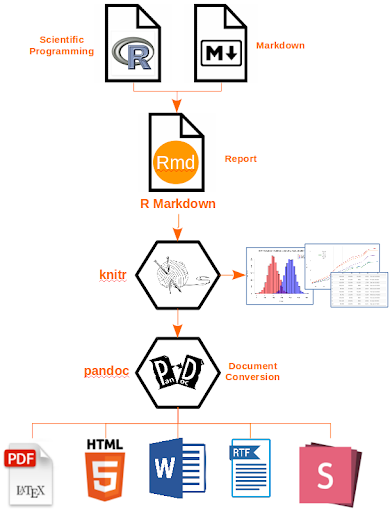
\includegraphics[width=0.6\linewidth]{figures/rmarkdown-flow} 

}

\caption{R Markdown의 최종 결과물 산출과정(http://applied-r.com/project-reporting-template/)}\label{fig:rmarkdown-flow}
\end{figure}

\normalsize

\hypertarget{create-rmd-file}{%
\subsubsection*{R Markdown 문서 시작하기}\label{create-rmd-file}}


\begin{itemize}
\tightlist
\item
  \textbf{R Markdown} 문서 생성: \texttt{{[}File{]}\ -\textgreater{}\ {[}New\ File{]}\ -\textgreater{}\ {[}R\ Markdown..{]}}을 선택
\end{itemize}

\footnotesize

\BeginKnitrBlock{rmdcaution}
RStudio를 처음 설치하고 위와 같이 진행할 경우 아래와 같은 패키지 설치 여부를 묻는 팝업 창이 나타남. 패키지 설치 여부에 \texttt{{[}Yes{]}}를 클릭하면 R Markdown 문서 생성을 위해 필요한 패키지들이 자동으로 설치
\EndKnitrBlock{rmdcaution}

\normalsize

\footnotesize

\begin{center}\includegraphics[width=0.8\linewidth]{figures/rmarkdown-new-01} \end{center}

\normalsize

\begin{itemize}
\tightlist
\item
  설치 완료 후 R Markdown으로 생성할 최종 문서 유형 선택 질의 창이 나타남. 아래 창에서 제목(Title)과 저자(Author) 이름 입력 후 \texttt{{[}OK{]}} 버튼 클릭(\texttt{Document}, \texttt{html} 문서 선택)
\end{itemize}

\footnotesize

\begin{center}\includegraphics[width=0.8\linewidth]{figures/rmarkdown-new-02} \end{center}

\normalsize

\begin{itemize}
\tightlist
\item
  아래 그림과 같이 새로운 문서 창이 생성되고 \texttt{test.Rmd} 파일로 저장\footnote{\protect\hyperlink{rstudio-project}{RStudio 프로젝트}에서 생성한 폴더 내에 파일 저장}
\end{itemize}

\footnotesize

\begin{center}\includegraphics[width=0.8\linewidth]{figures/rmarkdown-new-03} \end{center}

\normalsize

\begin{itemize}
\tightlist
\item
  문서 상단에 \texttt{Knit} 아이콘을 클릭 후 \texttt{Knit\ to\ HTML} 클릭 또는 문서 아무 곳에 커서를 위치하고 단축키 \texttt{{[}Ctrl{]}\ +\ {[}Shift{]}\ +\ {[}K{]}} 입력
\end{itemize}

\footnotesize

\begin{center}\includegraphics[width=0.8\linewidth]{figures/rmarkdown-new-04} \end{center}

\normalsize

\begin{itemize}
\tightlist
\item
  \texttt{knitr} + \texttt{R\ Markdown} + \texttt{pandoc} \(\rightarrow\) \texttt{html} 파일 생성 결과
\end{itemize}

\footnotesize

\begin{figure}

{\centering \includegraphics[width=0.8\linewidth]{figures/rmarkdown-new-out} 

}

\caption{test.html 문서 화면(저장 폴더 내 `test.html`을 크롬 브라우저로 실행)}\label{fig:rmarkdown-new-out}
\end{figure}

\normalsize

\hypertarget{r-markdown-uxbb38uxc11c-uxad6cuxc131}{%
\subsubsection{R Markdown 문서 구성}\label{r-markdown-uxbb38uxc11c-uxad6cuxc131}}

R Markdown 문서는 아래 그림과 같이 \textbf{YAML}, \textbf{Markdown 텍스트}, \textbf{Code Chunk} 세 부분으로 구성됨.

\footnotesize

\begin{center}\includegraphics[width=0.8\linewidth]{figures/rmarkdown-part} \end{center}

\normalsize

\textbf{1. YAML (YAML Ain't Markup Language)}

\begin{itemize}
\tightlist
\item
  R Markdown 문서의 metadata로 문서의 맨 처음에 항상 포함되어야 함.
\item
  R Markdown 문서의 최종 출력 형태, 제목, 저자, 날짜 등의 정보 등을 포함
\item
  YAML 언어에 대한 사용 예시는 \citet{xie-2016} 의 \href{https://bookdown.org/yihui/bookdown/r-markdown.html}{Appendix B.2} 참고
\item
  최소 형태의 YAML 예시
\end{itemize}

\footnotesize

\begin{Shaded}
\begin{Highlighting}[]
\OtherTok{---}
\FunctionTok{title:}\AttributeTok{ }\StringTok{"Hello R Markdown"}
\FunctionTok{author:}\AttributeTok{ }\StringTok{"Zorba"}
\FunctionTok{date:}\AttributeTok{ }\StringTok{"2020-03-17"}
\FunctionTok{output:}\AttributeTok{ html_document}
\OtherTok{---}
\end{Highlighting}
\end{Shaded}

\normalsize

\textbf{2. Markdown 텍스트}

\begin{itemize}
\tightlist
\item
  Markdown 문법은 15주 차 강의에서 배울 예정임
\item
  \href{https://rstudio.com/wp-content/uploads/2015/03/rmarkdown-reference.pdf}{R Markdown 레퍼런스 가이드} 참조
\item
  그림 삽입: \texttt{!{[}{]}(path/filename)}
\end{itemize}

\begin{Shaded}
\begin{Highlighting}[]
\NormalTok{그립 삽입 구문}
\NormalTok{![](figures/son.jpg)   }
\end{Highlighting}
\end{Shaded}

\includegraphics{figures/son.jpg}

\textbf{3. Code Chunk}

\begin{itemize}
\tightlist
\item
  실제 R code가 실행되는 부분임
\item
  Code chunk 실행 시 다양한 옵션들이 있으나 이 부분 역시 15주 차 강의에서 간략히 다룰 예정임
\item
  Code chunk는 \texttt{\textasciigrave{}\textasciigrave{}\textasciigrave{}\{r\}}로 시작되며 \texttt{r}은 code 언어 이름을 나타냄.
\item
  Code chunk는 \texttt{\textasciigrave{}\textasciigrave{}\textasciigrave{}} 로 종료
\item
  R Markdown 문서 작성 시 단축키 \texttt{{[}Ctrl{]}\ +\ {[}Alt{]}\ +\ {[}I{]}}를 입력하면 Chunk 입력창이 자동 생성됨
\item
  Chunk option에 대한 상세 내용은 \url{https://yihui.org/knitr/options/} 또는 \href{https://rstudio.com/wp-content/uploads/2015/03/rmarkdown-reference.pdf}{R Markdown 레퍼런스 가이드} 참조
\end{itemize}

\begin{Shaded}
\begin{Highlighting}[]
\NormalTok{Code chunk 예시}

\NormalTok{Xie의 R Markdown: The Definitive Guide에서 발췌}

\BaseNTok{```\{r\}}
\BaseNTok{fit = lm(dist ~ speed, data = cars)}
\BaseNTok{b   = coef(fit)}
\BaseNTok{plot(cars)}
\BaseNTok{abline(fit)}
\BaseNTok{```}
\end{Highlighting}
\end{Shaded}

\footnotesize

\begin{Shaded}
\begin{Highlighting}[]
\NormalTok{fit =}\StringTok{ }\KeywordTok{lm}\NormalTok{(dist }\OperatorTok{~}\StringTok{ }\NormalTok{speed, }\DataTypeTok{data =}\NormalTok{ cars)}
\NormalTok{b   =}\StringTok{ }\KeywordTok{coef}\NormalTok{(fit)}
\KeywordTok{plot}\NormalTok{(cars)}
\KeywordTok{abline}\NormalTok{(fit)}
\end{Highlighting}
\end{Shaded}

\includegraphics{01-overview_files/figure-latex/unnamed-chunk-44-1.pdf}

\normalsize

\begin{itemize}
\tightlist
\item
  Code chunk에서 외부 그림 파일 불러오기(\citet{xie-2018} 에서 예시 발췌)
\end{itemize}

\footnotesize

\begin{Shaded}
\begin{Highlighting}[]
\NormalTok{knitr}\OperatorTok{::}\KeywordTok{include_graphics}\NormalTok{(}\KeywordTok{rep}\NormalTok{(}\StringTok{'figures/knit-logo.png'}\NormalTok{, }\DecValTok{3}\NormalTok{))}
\end{Highlighting}
\end{Shaded}

\includegraphics[width=0.328\linewidth]{figures/knit-logo} \includegraphics[width=0.328\linewidth]{figures/knit-logo} \includegraphics[width=0.328\linewidth]{figures/knit-logo}

\normalsize

\footnotesize

\BeginKnitrBlock{rmdimportant}
\textbf{Homework 1}: R Markdown 문서에 아래 내용을 포함한 문서를 \texttt{html} 파일 형식으로 출력 후 제출

\begin{itemize}
\tightlist
\item
  간략한 자기소개 및 ``통계 프로그래밍 언어'' 수업에 대한 본인만의 목표 기술
\item
  본인이 setting 한 RStudio 구성 캡쳐 화면을 그림 파일로 저장하고 R Markdown 문서에 삽입(화면 캡쳐 시 생성 프로젝트 내 폴더 내용 반드시 포함)
\item
  패키지 \texttt{ggplot2}를 불러오고 \texttt{cars} 데이터셋의 2차원 산점도(\textbf{hint}: \texttt{help(geom\_point)} 또는 googling 활용)를 문서에 포함
\end{itemize}
\EndKnitrBlock{rmdimportant}

\normalsize

\hypertarget{data-type}{%
\chapter{R 객체(R object)}\label{data-type}}

\footnotesize

\BeginKnitrBlock{rmdnote}
\textbf{학습목표(2 주차)}: R에서 사용 가능한 데이터 타입에 대해 알아보고, 고유 데이터 타입으로 구성한 객체(스칼라, 백터, 리스트)와 이와 연관된 함수들을 익힌다.
\EndKnitrBlock{rmdnote}

\normalsize

\hypertarget{ch2-abstract}{%
\subsubsection*{학습 필요성}\label{ch2-abstract}}


\begin{itemize}
\tightlist
\item
  R언어는 타 프로그래밍 언어와 유사한 데이터 타입(정수형, 실수형, 문자형 등)을 제공
\item
  R 언어가 다른 언어와 차이점 \(\rightarrow\) \textbf{데이터 분석}에 특화된 벡터(vector), 행렬(matrix), 데이터프레임(data frame), 리스트(list)와 같은 객체\footnote{R에서 사용자가 데이터 입력을 위해 생성 또는 읽어온 객체(object)는 종종 변수(variable)라는 말과 혼용. 본 문서에서는 최상위 데이터 저장장소를 객체라고 명명하며 데이터프레임과 같이 여러 종류의 데이터타입으로 이루어진 객체의 1차원 속성을 변수라고 칭함} 제공
\item
  R 패키지에서 제공되는 함수 사용 방법은 R의 객체에 따라 달라질 수 있음\\
\item
  R 언어를 원활히 다룰 수 있으려면 R에서 데이터 객체의 형태, 자료 할당 및 그 연산 방법에 대한 이해가 필수적으로 선행되어야 함
\end{itemize}

\hypertarget{object-value}{%
\subsubsection*{R의 데이터 타입}\label{object-value}}


\begin{itemize}
\item
  \textbf{수치형(numeric)}: 숫자(정수, 소수)
\item
  \textbf{문자열(string)}: \texttt{"충남대학교"}, \texttt{"R강의"}
\item
  \textbf{논리형(logical)}: \texttt{TRUE}/\texttt{FALSE}
\item
  \textbf{결측값(\texttt{NA})}: 자료에서 발생한 결측 표현
\item
  \textbf{공백(\texttt{NULL})}: 지정하지 않은 값
\item
  \textbf{요인(factor)}: 범주형 자료 표현(수치 + 문자 결합 형태로 이해하면 편함)
\item
  \textbf{기타}: 숫자아님(\texttt{NaN}), 무한대(\texttt{Inf}) 등
\end{itemize}

\hypertarget{ch2-object-type}{%
\subsubsection*{R 객체의 종류}\label{ch2-object-type}}


\begin{itemize}
\tightlist
\item
  스칼라(상수형, scalar 또는 atomic)
\item
  벡터(vector): \textbf{R의 기본연산 단위}
\item
  리스트(list)
\item
  행렬(matrix)
\item
  배열(array)
\item
  데이터프레임(data frame)
\end{itemize}

\textbf{아래 그림은 2\textasciitilde4 주차에 배울 R 주요 객체에 대한 개요도임}

\footnotesize

\begin{figure}

{\centering \includegraphics[width=1\linewidth]{figures/datatype-diagram} 

}

\caption{R 데이터 타입 구조 다이어그램: [R, Python 분석과 프로그래밍 (by R Friend)]( http://rfriend.tistory.com/)에서 발췌 후 수정}\label{fig:rmarkdown-part}
\end{figure}

\normalsize

\hypertarget{scalar}{%
\section{스칼라(scalar)}\label{scalar}}

\begin{itemize}
\tightlist
\item
  단일 차원의 값(하나의 값): \(1 \times 1\) 백터로 표현 \(\rightarrow\) R 데이터 객체의 기본은 벡터!!
\item
  데이터 객체의 유형은 크게 숫자형, 문자열, 논리형이 있음
\end{itemize}

\footnotesize

\BeginKnitrBlock{rmdtip}
스칼라를 입력시 R의 벡터 지정 함수인 \texttt{c()}(벡터 부분에서 상세 내용 학습)를 꼭 사용해서 입력할 필요가 없다. 단, 연속되지 않은 두 개 이상 스칼라면 벡터이므로 꼭 c()를 써야 한다.
\EndKnitrBlock{rmdtip}

\normalsize

\hypertarget{definition}{%
\subsection{선언}\label{definition}}

\begin{itemize}
\tightlist
\item
  일반적으로 컴파일이 필요한 언어(예: \texttt{C} 언어)의 경우 변수 또는 객체를 사용 전에 선언이 필요
\end{itemize}

\footnotesize

\begin{Shaded}
\begin{Highlighting}[]
\DataTypeTok{int}\NormalTok{ x; }
\NormalTok{x = }\DecValTok{1}\NormalTok{;}
\end{Highlighting}
\end{Shaded}

\normalsize

\begin{itemize}
\item
  위 코드에서 \texttt{int\ x;} 없이 \texttt{x\ =\ 1}을 입력 후 컴파일 하면 에러가 나타나지만 \texttt{R} 언어에서는 \textbf{변수를 선언할 필요가 전혀 없음}
\item
  \texttt{z} 가 어떤 데이터 타입인지 언급할 필요가 전혀 없음 \(\rightarrow\) \texttt{Python}, \texttt{Perl}, \texttt{Matlab} 등과 같은 스크립트 언어의 특징. 아래 코드 참조
\end{itemize}

\footnotesize

\begin{Shaded}
\begin{Highlighting}[]
\NormalTok{z <-}\StringTok{ }\DecValTok{3}
\NormalTok{z}
\end{Highlighting}
\end{Shaded}

\begin{verbatim}
[1] 3
\end{verbatim}

\normalsize

\hypertarget{numeric}{%
\subsection{숫자형}\label{numeric}}

\begin{itemize}
\tightlist
\item
  정수형(integer)과 실수형(double)로 구분됨
\item
  정수형 구분시 숫자 뒤 \texttt{L}을 표시
\end{itemize}

\footnotesize

\begin{Shaded}
\begin{Highlighting}[]
\CommentTok{# 정수형 구분자 사용 예시}
\CommentTok{# typeof(): R 객체의 데이터 타입 반환하는 함수}
\KeywordTok{typeof}\NormalTok{(10L)}
\end{Highlighting}
\end{Shaded}

\begin{verbatim}
[1] "integer"
\end{verbatim}

\begin{Shaded}
\begin{Highlighting}[]
\KeywordTok{typeof}\NormalTok{(}\DecValTok{10}\NormalTok{)}
\end{Highlighting}
\end{Shaded}

\begin{verbatim}
[1] "double"
\end{verbatim}

\normalsize

\begin{itemize}
\tightlist
\item
  수치연산(\texttt{+,\ -,\ *,\ \^{},\ **,\ /,\ \%\%,\ \%/\%}) 가능: R은 함수형 언어이기 때문에 앞에 기술한 연산자도 하나의 함수로 인식함.
\item
  수치 연산자(operator) 및 기본 수학 함수
\end{itemize}

\footnotesize

\begin{table}[H]

\caption{\label{tab:operation}R언어의 기본 수치 연산자}
\centering
\fontsize{10}{12}\selectfont
\begin{tabular}[t]{>{\raggedright\arraybackslash}p{4cm}>{\raggedright\arraybackslash}p{6cm}}
\toprule
수치형 연산자 & 설명\\
\midrule
\rowcolor{gray!6}  \ttfamily{+, -, *, /} & \ttfamily{사칙연산}\\
\ttfamily{n \%\% m} & \ttfamily{n을 m 으로 나눈 나머지}\\
\rowcolor{gray!6}  \ttfamily{n \%/\% m} & \ttfamily{n을 m 으로 나눈 몫}\\
\ttfamily{n \textasciicircum{} m 또는 n ** m} & \ttfamily{n 의 m 승}\\
\bottomrule
\end{tabular}
\end{table}

\normalsize

\textbf{숫자형 스칼라 연산 적용 예시}

\footnotesize

\begin{Shaded}
\begin{Highlighting}[]
\CommentTok{# 숫자형 스칼라}
\NormalTok{a <-}\StringTok{ }\DecValTok{3}
\NormalTok{b <-}\StringTok{ }\DecValTok{10}
\NormalTok{a; b}
\end{Highlighting}
\end{Shaded}

\begin{verbatim}
[1] 3
\end{verbatim}

\begin{verbatim}
[1] 10
\end{verbatim}

\begin{Shaded}
\begin{Highlighting}[]
\CommentTok{# 덧셈}
\NormalTok{c <-}\StringTok{ }\NormalTok{a }\OperatorTok{+}\StringTok{ }\NormalTok{b}
\NormalTok{c}
\end{Highlighting}
\end{Shaded}

\begin{verbatim}
[1] 13
\end{verbatim}

\begin{Shaded}
\begin{Highlighting}[]
\CommentTok{# 덧셈을 함수로 입력}
\CommentTok{# "+"(a, b)로 입력한 결과}
\NormalTok{c <-}\StringTok{ "+"}\NormalTok{(a, b)}

\CommentTok{# 뺄셈}
\NormalTok{d <-}\StringTok{ }\NormalTok{b }\OperatorTok{-}\StringTok{ }\NormalTok{a}
\NormalTok{d}
\end{Highlighting}
\end{Shaded}

\begin{verbatim}
[1] 7
\end{verbatim}

\begin{Shaded}
\begin{Highlighting}[]
\CommentTok{# 곱셈}
\NormalTok{m <-}\StringTok{ }\NormalTok{a }\OperatorTok{*}\StringTok{ }\NormalTok{b}
\NormalTok{m}
\end{Highlighting}
\end{Shaded}

\begin{verbatim}
[1] 30
\end{verbatim}

\begin{Shaded}
\begin{Highlighting}[]
\CommentTok{# 나누기}
\NormalTok{dd <-}\StringTok{ }\NormalTok{b}\OperatorTok{/}\NormalTok{a}
\NormalTok{dd}
\end{Highlighting}
\end{Shaded}

\begin{verbatim}
[1] 3.333333
\end{verbatim}

\begin{Shaded}
\begin{Highlighting}[]
\CommentTok{# 멱승}
\NormalTok{b}\OperatorTok{^}\NormalTok{a}
\end{Highlighting}
\end{Shaded}

\begin{verbatim}
[1] 1000
\end{verbatim}

\begin{Shaded}
\begin{Highlighting}[]
\CommentTok{# 나누기의 나머지(remainder) 반환}
\NormalTok{r <-}\StringTok{ }\NormalTok{b }\OperatorTok\StringTok{ }\NormalTok{a}
\NormalTok{r}
\end{Highlighting}
\end{Shaded}

\begin{verbatim}
[1] 1
\end{verbatim}

\begin{Shaded}
\begin{Highlighting}[]
\CommentTok{# 나누기의 몫(quotient) 반환}
\NormalTok{q <-}\StringTok{ }\NormalTok{b }\OperatorTok\StringTok{ }\NormalTok{a}
\NormalTok{q}
\end{Highlighting}
\end{Shaded}

\begin{verbatim}
[1] 3
\end{verbatim}

\begin{Shaded}
\begin{Highlighting}[]
\CommentTok{# 연산 우선 순위}
\NormalTok{nn <-}\StringTok{ }\NormalTok{(}\DecValTok{3} \OperatorTok{+}\StringTok{ }\DecValTok{5}\NormalTok{)}\OperatorTok{*}\DecValTok{3} \OperatorTok{-}\StringTok{ }\DecValTok{4}\OperatorTok{**}\DecValTok{2}\OperatorTok{/}\DecValTok{4}
\NormalTok{nn}
\end{Highlighting}
\end{Shaded}

\begin{verbatim}
[1] 20
\end{verbatim}

\normalsize

\hypertarget{character}{%
\subsection{문자형}\label{character}}

\begin{itemize}
\tightlist
\item
  수치형이 아닌 문자 형식의 단일 원소
\item
  C와 같은 언어에서 볼수 있는 한개 문자에 대한 데이터 타입 존재하지 않음
\item
  수치연산 불가능
\item
  따옴표(\texttt{"} 또는 \texttt{\textquotesingle{}})로 문자를 묶어서 문자열 표시
\item
  문자열을 다루는 자세한 설명은 5주차에서 자세히 설명할 예정임
\end{itemize}

\footnotesize

\begin{Shaded}
\begin{Highlighting}[]
\NormalTok{h1 <-}\StringTok{ }\KeywordTok{c}\NormalTok{(}\StringTok{"Hello CNU!!"}\NormalTok{)}
\NormalTok{h2 <-}\StringTok{ }\KeywordTok{c}\NormalTok{(}\StringTok{"R is not too difficult."}\NormalTok{)}
\KeywordTok{typeof}\NormalTok{(h1); }\KeywordTok{typeof}\NormalTok{(h2)}
\end{Highlighting}
\end{Shaded}

\begin{verbatim}
[1] "character"
\end{verbatim}

\begin{verbatim}
[1] "character"
\end{verbatim}

\begin{Shaded}
\begin{Highlighting}[]
\NormalTok{h1}
\end{Highlighting}
\end{Shaded}

\begin{verbatim}
[1] "Hello CNU!!"
\end{verbatim}

\begin{Shaded}
\begin{Highlighting}[]
\NormalTok{h2}
\end{Highlighting}
\end{Shaded}

\begin{verbatim}
[1] "R is not too difficult."
\end{verbatim}

\begin{Shaded}
\begin{Highlighting}[]
\CommentTok{# 문자열의 문자 수 반환}
\KeywordTok{nchar}\NormalTok{(h1); }\KeywordTok{nchar}\NormalTok{(h2)}
\end{Highlighting}
\end{Shaded}

\begin{verbatim}
[1] 11
\end{verbatim}

\begin{verbatim}
[1] 23
\end{verbatim}

\begin{Shaded}
\begin{Highlighting}[]
\CommentTok{# 문자열 연산 error 예시}
\NormalTok{h1 }\OperatorTok{-}\StringTok{ }\NormalTok{h2}
\end{Highlighting}
\end{Shaded}

\begin{verbatim}
Error in h1 - h2: 이항연산자에 수치가 아닌 인수입니다
\end{verbatim}

\normalsize

\hypertarget{logical}{%
\subsection{논리형 스칼라}\label{logical}}

\begin{itemize}
\tightlist
\item
  참(\texttt{TRUE}, \texttt{T}) 또는 거짓(\texttt{FALSE}, \texttt{F})를 나타내는 값
\item
  \texttt{TRUE}/\texttt{FALSE}: 예약어(reversed word)
\item
  \texttt{T}/\texttt{F}: \texttt{TRUE}와 \texttt{FALSE}로 초기화된 전역 변수

  \begin{itemize}
  \tightlist
  \item
    \texttt{T}에 \texttt{FALSE} 또는 어떤 값도 할당 가능 \(\rightarrow\) 가급적 \texttt{TRUE/FALSE}를 명시하는 것이 편함
  \end{itemize}
\item
  논리형 연산자(logical operator)
\end{itemize}

\footnotesize

\begin{table}[H]

\caption{\label{tab:logic-op-tab}R언어의 논리형 연산자}
\centering
\fontsize{10}{12}\selectfont
\begin{tabular}[t]{>{\raggedright\arraybackslash}p{3cm}>{\raggedright\arraybackslash}p{7cm}}
\toprule
논리형 연산자 & 설명\\
\midrule
\rowcolor{gray!6}  \ttfamily{\&} & \ttfamily{AND (vectorized)}\\
\ttfamily{\&\&} & \ttfamily{AND (atomic)}\\
\rowcolor{gray!6}  \ttfamily{|} & \ttfamily{OR (vectorized)}\\
\ttfamily{||} & \ttfamily{OR (atomic)}\\
\rowcolor{gray!6}  \ttfamily{!} & \ttfamily{NOT}\\
\bottomrule
\end{tabular}
\end{table}

\normalsize

\begin{itemize}
\tightlist
\item
  비교 연산자를 적용할 경우 논리값을 반환
\end{itemize}

\footnotesize

\begin{table}[H]

\caption{\label{tab:comp-op-tab}R언어의 비교 연산자}
\centering
\fontsize{10}{12}\selectfont
\begin{threeparttable}
\begin{tabular}[t]{>{\raggedright\arraybackslash}p{3cm}>{\raggedright\arraybackslash}p{7cm}}
\toprule
비교 연산자 & 설명\\
\midrule
\rowcolor{gray!6}  \ttfamily{>} & \ttfamily{크다(greater-than)}\\
\ttfamily{<} & \ttfamily{작다(less-than)}\\
\rowcolor{gray!6}  \ttfamily{==} & \ttfamily{같다(equal)}\\
\ttfamily{>=} & \ttfamily{크거나 같다(greater than equal)}\\
\rowcolor{gray!6}  \ttfamily{<=} & \ttfamily{작거나 같다(less than equal)}\\
\addlinespace
\ttfamily{!=} & \ttfamily{같지 않다(not equal)}\\
\bottomrule
\end{tabular}
\begin{tablenotes}
\item \textit{Note: } 
\item 기술한 비교 연산자는 수치형 및 논리형 데이터 타입 모두에 적용 가능 하지만, 문자형은 비교 연산은 ==, != 만 가능함
\end{tablenotes}
\end{threeparttable}
\end{table}

\normalsize

\footnotesize

\BeginKnitrBlock{rmdnote}
\textbf{참고}

\begin{itemize}
\tightlist
\item
  논리형 스칼라도 숫자형 연산 가능 \(\rightarrow\) 컴퓨터는 \texttt{TRUE}/\texttt{FALSE}를 1과 0 숫자로 인식
\item
  수치 연산자는 스칼라 뿐 아니라 아래에서 다룰 벡터, 행렬, 리스트, 데이터프레임 객체의 연산에 사용 가능
\item
  \texttt{\&}/\texttt{\textbar{}}와 \texttt{\&\&}/\texttt{\textbar{}\textbar{}}는 동일하게 AND/OR를 의미하지만 연산 결과가 다름.
\item
  \texttt{\&}의 연산 대상이 벡터인 경우 백터 구성 값 각각에 대해 \texttt{\&} 연산을 실행 하지만 \texttt{\&\&}는 하나의 값(스칼라)에만 논리 연산이 적용(아래 예시 참고)
\end{itemize}
\EndKnitrBlock{rmdnote}

\normalsize

\begin{itemize}
\tightlist
\item
  논리형 스칼라의 논리 및 비교 연산 예시
\end{itemize}

\footnotesize

\begin{Shaded}
\begin{Highlighting}[]
\KeywordTok{typeof}\NormalTok{(}\OtherTok{TRUE}\NormalTok{)  }\CommentTok{# TRUE의 데이터 타입}
\end{Highlighting}
\end{Shaded}

\begin{verbatim}
[1] "logical"
\end{verbatim}

\begin{Shaded}
\begin{Highlighting}[]
\OtherTok{TRUE} \OperatorTok{&}\StringTok{ }\OtherTok{TRUE}  \CommentTok{# TRUE 반환}
\end{Highlighting}
\end{Shaded}

\begin{verbatim}
[1] TRUE
\end{verbatim}

\begin{Shaded}
\begin{Highlighting}[]
\OtherTok{TRUE} \OperatorTok{&}\StringTok{ }\OtherTok{FALSE}  \CommentTok{# FALSE 반환}
\end{Highlighting}
\end{Shaded}

\begin{verbatim}
[1] FALSE
\end{verbatim}

\begin{Shaded}
\begin{Highlighting}[]
\CommentTok{# 아래 연산은 모두 TRUE 반환}
\OtherTok{TRUE} \OperatorTok{|}\StringTok{ }\OtherTok{TRUE}
\end{Highlighting}
\end{Shaded}

\begin{verbatim}
[1] TRUE
\end{verbatim}

\begin{Shaded}
\begin{Highlighting}[]
\OtherTok{TRUE} \OperatorTok{|}\StringTok{ }\OtherTok{FALSE}
\end{Highlighting}
\end{Shaded}

\begin{verbatim}
[1] TRUE
\end{verbatim}

\begin{Shaded}
\begin{Highlighting}[]
\CommentTok{# TRUE와 FALSE의 반대}
\OperatorTok{!}\OtherTok{TRUE}
\end{Highlighting}
\end{Shaded}

\begin{verbatim}
[1] FALSE
\end{verbatim}

\begin{Shaded}
\begin{Highlighting}[]
\OperatorTok{!}\OtherTok{FALSE}
\end{Highlighting}
\end{Shaded}

\begin{verbatim}
[1] TRUE
\end{verbatim}

\begin{Shaded}
\begin{Highlighting}[]
\CommentTok{# 전역변수 T에 FALSE 값 할당}
\NormalTok{T <-}\StringTok{ }\OtherTok{FALSE}
\NormalTok{T}
\end{Highlighting}
\end{Shaded}

\begin{verbatim}
[1] FALSE
\end{verbatim}

\begin{Shaded}
\begin{Highlighting}[]
\NormalTok{T <-}\StringTok{ }\OtherTok{TRUE}  \CommentTok{# 원상복귀}
\CommentTok{# TRUE/FALSE에 값을 할당할 수 없음}
\OtherTok{TRUE}\NormalTok{ <-}\StringTok{ }\DecValTok{1}
\end{Highlighting}
\end{Shaded}

\begin{verbatim}
Error in TRUE <- 1: 대입에 유효하지 않은 (do_set) 좌변입니다
\end{verbatim}

\begin{Shaded}
\begin{Highlighting}[]
\OtherTok{TRUE}\NormalTok{ <-}\StringTok{ }\OtherTok{FALSE}
\end{Highlighting}
\end{Shaded}

\begin{verbatim}
Error in TRUE <- FALSE: 대입에 유효하지 않은 (do_set) 좌변입니다
\end{verbatim}

\begin{Shaded}
\begin{Highlighting}[]
\CommentTok{# &(|)와 &&(||)의 차이}
\NormalTok{l}\FloatTok{.01}\NormalTok{ <-}\StringTok{ }\KeywordTok{c}\NormalTok{(}\OtherTok{TRUE}\NormalTok{, }\OtherTok{TRUE}\NormalTok{, }\OtherTok{FALSE}\NormalTok{, }\OtherTok{TRUE}\NormalTok{)  }\CommentTok{# 논리형 값으로 구성된 벡터}
\NormalTok{l}\FloatTok{.02}\NormalTok{ <-}\StringTok{ }\KeywordTok{c}\NormalTok{(}\OtherTok{FALSE}\NormalTok{, }\OtherTok{TRUE}\NormalTok{, }\OtherTok{TRUE}\NormalTok{, }\OtherTok{TRUE}\NormalTok{)}
\NormalTok{l}\FloatTok{.01} \OperatorTok{&}\StringTok{ }\NormalTok{l}\FloatTok{.02}  \CommentTok{# l.01과 l.02 각 원소 별 & 연산}
\end{Highlighting}
\end{Shaded}

\begin{verbatim}
[1] FALSE  TRUE FALSE  TRUE
\end{verbatim}

\begin{Shaded}
\begin{Highlighting}[]
\NormalTok{l}\FloatTok{.01} \OperatorTok{&&}\StringTok{ }\NormalTok{l}\FloatTok{.02}  \CommentTok{# l.01과 l.02의 첫 번째 원소에 대해 & 연산}
\end{Highlighting}
\end{Shaded}

\begin{verbatim}
[1] FALSE
\end{verbatim}

\begin{Shaded}
\begin{Highlighting}[]
\CommentTok{# 비교 연산자}
\NormalTok{x <-}\StringTok{ }\DecValTok{9}
\NormalTok{y <-}\StringTok{ }\DecValTok{4}
\CommentTok{# x > y 의 반환값 데이터 타입}
\KeywordTok{typeof}\NormalTok{(x }\OperatorTok{>}\StringTok{ }\NormalTok{y)}
\end{Highlighting}
\end{Shaded}

\begin{verbatim}
[1] "logical"
\end{verbatim}

\begin{Shaded}
\begin{Highlighting}[]
\CommentTok{# 논리형 값 반환}
\NormalTok{x }\OperatorTok{>}\StringTok{ }\NormalTok{y}
\end{Highlighting}
\end{Shaded}

\begin{verbatim}
[1] TRUE
\end{verbatim}

\begin{Shaded}
\begin{Highlighting}[]
\NormalTok{x }\OperatorTok{<}\StringTok{ }\NormalTok{y}
\end{Highlighting}
\end{Shaded}

\begin{verbatim}
[1] FALSE
\end{verbatim}

\begin{Shaded}
\begin{Highlighting}[]
\NormalTok{x }\OperatorTok{==}\StringTok{ }\NormalTok{y}
\end{Highlighting}
\end{Shaded}

\begin{verbatim}
[1] FALSE
\end{verbatim}

\begin{Shaded}
\begin{Highlighting}[]
\NormalTok{x }\OperatorTok{!=}\StringTok{ }\NormalTok{y}
\end{Highlighting}
\end{Shaded}

\begin{verbatim}
[1] TRUE
\end{verbatim}

\normalsize

\hypertarget{missing-value}{%
\subsection{결측값(missing value)}\label{missing-value}}

\begin{itemize}
\tightlist
\item
  결측치 지정 \textbf{상수}: \texttt{NA} \(\rightarrow\) R과 다른 언어의 가장 큰 차이점 중 하나
\item
  예를 들어 4명의 통계학과 학생 중 3명의 통계학 개론 중간고사 점수가 각각 80, 90, 75점이고 4번 째 학생의 점수가 없는 경우 \texttt{NA}로 결측값 표현
\item
  \texttt{is.na()} 함수를 이용해 해당 값이 결측을 포함하고 있는지 확인
\end{itemize}

\footnotesize

\begin{Shaded}
\begin{Highlighting}[]
\NormalTok{one <-}\StringTok{ }\DecValTok{80}\NormalTok{; two <-}\StringTok{ }\DecValTok{90}\NormalTok{; three <-}\StringTok{ }\DecValTok{75}\NormalTok{; four <-}\StringTok{ }\OtherTok{NA}
\NormalTok{four}
\end{Highlighting}
\end{Shaded}

\begin{verbatim}
[1] NA
\end{verbatim}

\begin{Shaded}
\begin{Highlighting}[]
\CommentTok{# 'is.na()' 결측 NA가 포함되어 있으면 TRUE }
\KeywordTok{is.na}\NormalTok{(four)}
\end{Highlighting}
\end{Shaded}

\begin{verbatim}
[1] TRUE
\end{verbatim}

\normalsize

\footnotesize

\BeginKnitrBlock{rmdtip}
\texttt{is.na(object\_name)}: 객체를 구성하고 있는 원소 중 \texttt{NA}를 포함하고 있는지 확인 \(\rightarrow\) \texttt{NA}를 포함하면 \texttt{TRUE}, 아니면 \texttt{FALSE} 반환

\textbf{참고}: 자료에 \texttt{NA}가 포함된 경우 연산 결과는 모두 \texttt{NA}가 반환
\EndKnitrBlock{rmdtip}

\normalsize

\footnotesize

\begin{Shaded}
\begin{Highlighting}[]
\OtherTok{NA} \OperatorTok{+}\StringTok{ }\DecValTok{1}
\end{Highlighting}
\end{Shaded}

\begin{verbatim}
[1] NA
\end{verbatim}

\begin{Shaded}
\begin{Highlighting}[]
\OtherTok{NA} \OperatorTok{&}\StringTok{ }\OtherTok{TRUE}
\end{Highlighting}
\end{Shaded}

\begin{verbatim}
[1] NA
\end{verbatim}

\begin{Shaded}
\begin{Highlighting}[]
\OtherTok{NA} \OperatorTok{<=}\StringTok{ }\DecValTok{3}
\end{Highlighting}
\end{Shaded}

\begin{verbatim}
[1] NA
\end{verbatim}

\normalsize

\hypertarget{null}{%
\subsection{NULL 값}\label{null}}

\begin{itemize}
\tightlist
\item
  \texttt{NULL}: 초기화 되지 않은 변수 또는 \textbf{객체}를 지칭함
\item
  \texttt{is.null()} 함수를 통해 객체가 \texttt{NULL}인지 판단
\end{itemize}

\footnotesize

\begin{Shaded}
\begin{Highlighting}[]
\NormalTok{x <-}\StringTok{ }\OtherTok{NULL} \CommentTok{# NULL 지정}
\KeywordTok{is.null}\NormalTok{(x) }\CommentTok{# NULL 객체인지 판단}
\end{Highlighting}
\end{Shaded}

\begin{verbatim}
[1] TRUE
\end{verbatim}

\begin{Shaded}
\begin{Highlighting}[]
\NormalTok{x <-}\StringTok{ }\DecValTok{1}
\KeywordTok{is.null}\NormalTok{(x) }
\end{Highlighting}
\end{Shaded}

\begin{verbatim}
[1] FALSE
\end{verbatim}

\normalsize

\footnotesize

\BeginKnitrBlock{rmdnote}
\textbf{\texttt{NA}와 \texttt{NULL}의 차이점}: 자료의 공백을 의미한다는 점에서 유사한 측면이 있으나 아래 내용처럼 큰 차이가 있음

\begin{itemize}
\tightlist
\item
  \texttt{NULL}: 값을 지정하지 않은 객체를 표현하는데 사용. 즉 아직 변수 또는 객체의 상태가 아직 미정인 상태를 나타냄
\item
  \texttt{NA}: 데이터 값이 결측임을 지정해주는 논리형 상수
\end{itemize}
\EndKnitrBlock{rmdnote}

\normalsize

\footnotesize

\begin{Shaded}
\begin{Highlighting}[]
\CommentTok{# NA와 NULL은 다름}
\NormalTok{x <-}\StringTok{ }\OtherTok{NA}
\KeywordTok{is.null}\NormalTok{(}\OtherTok{NA}\NormalTok{)}
\end{Highlighting}
\end{Shaded}

\begin{verbatim}
[1] FALSE
\end{verbatim}

\begin{Shaded}
\begin{Highlighting}[]
\KeywordTok{is.na}\NormalTok{(}\OtherTok{NULL}\NormalTok{)}
\end{Highlighting}
\end{Shaded}

\begin{verbatim}
logical(0)
\end{verbatim}

\normalsize

\hypertarget{finite}{%
\subsection{무한대/무한소/숫자아님}\label{finite}}

\begin{itemize}
\tightlist
\item
  \texttt{Inf}: 무한대(\(+\infty\), \(1/0\))
\item
  \texttt{-Inf}: 무한소(\(-\infty\), \(-1/0\))
\item
  \texttt{NaN}: 숫자아님(Not a Number, \(0/0\))
\item
  \texttt{is.finite()}, \texttt{is.infinite()}, \texttt{is.nan()} 함수를 통해 객체가 \texttt{Inf} 또는 \texttt{NaN}을 포함하는지 확인
\end{itemize}

\footnotesize

\begin{Shaded}
\begin{Highlighting}[]
\NormalTok{x <-}\StringTok{ }\OtherTok{Inf}
\KeywordTok{is.finite}\NormalTok{(x)}
\end{Highlighting}
\end{Shaded}

\begin{verbatim}
[1] FALSE
\end{verbatim}

\begin{Shaded}
\begin{Highlighting}[]
\KeywordTok{is.infinite}\NormalTok{(x)}
\end{Highlighting}
\end{Shaded}

\begin{verbatim}
[1] TRUE
\end{verbatim}

\begin{Shaded}
\begin{Highlighting}[]
\NormalTok{x <-}\StringTok{ }\DecValTok{0}\OperatorTok{/}\DecValTok{0}
\KeywordTok{is.nan}\NormalTok{(x)}
\end{Highlighting}
\end{Shaded}

\begin{verbatim}
[1] TRUE
\end{verbatim}

\begin{Shaded}
\begin{Highlighting}[]
\KeywordTok{is.infinite}\NormalTok{(x)}
\end{Highlighting}
\end{Shaded}

\begin{verbatim}
[1] FALSE
\end{verbatim}

\normalsize

\footnotesize

\BeginKnitrBlock{rmdnote}
지금까지 요인형(factor)을 제외하고 R 언어에서 객체가 가질 수 있는 데이터 유형에 대해 알아봄. 요인형은 4주 차에 예정된 ``R 자료형: 팩터, 테이블, 데이터 프레임''에서 상세하게 배울 예정임.
\EndKnitrBlock{rmdnote}

\normalsize

\hypertarget{vector}{%
\section{벡터(vector)}\label{vector}}

\hypertarget{vector-prop}{%
\subsection{벡터의 특징}\label{vector-prop}}

\begin{itemize}
\tightlist
\item
  타 프로그래밍 언어의 배열(array)의 개념으로 \textbf{동일한 유형}의 데이터 원소가 하나 이상(\(n \times 1\), \(n \geq 1\)) 으로 구성된 자료 형태
\item
  R 언어의 가장 기본적인 데이터 형태로 R에서 행해지는 모든 연산의 기본(vectorization) \(\rightarrow\) 벡터 연산 시 반복구문(예: \texttt{for\ loop})이 필요 없음.
\item
  \ref{scalar} 절에서 기술한 \protect\hyperlink{scalar}{스칼라(scalar)}는 사실 \(1 \times 1\) 벡터임
\item
  수학적으로 벡터는 아래와 같이 나타낼 수 있음
\end{itemize}

\[\mathrm{\mathbf x} = [x_1, x_2, x_3, \ldots, x_n]^T
\]

\begin{itemize}
\tightlist
\item
  벡터는 앞의 예시에서 본 바와 같이 \texttt{c()} 함수를 사용해 생성
\end{itemize}

\footnotesize

\begin{Shaded}
\begin{Highlighting}[]
\CommentTok{# 숫자형 벡터 }
\NormalTok{x <-}\StringTok{ }\KeywordTok{c}\NormalTok{(}\DecValTok{2}\NormalTok{, }\DecValTok{0}\NormalTok{, }\DecValTok{2}\NormalTok{, }\DecValTok{0}\NormalTok{, }\DecValTok{0}\NormalTok{, }\DecValTok{3}\NormalTok{, }\DecValTok{2}\NormalTok{, }\DecValTok{4}\NormalTok{)}
\NormalTok{x}
\end{Highlighting}
\end{Shaded}

\begin{verbatim}
[1] 2 0 2 0 0 3 2 4
\end{verbatim}

\begin{Shaded}
\begin{Highlighting}[]
\CommentTok{# 문자형 벡터}
\NormalTok{y <-}\StringTok{ }\KeywordTok{c}\NormalTok{(}\StringTok{"Boncho Ku"}\NormalTok{, }\StringTok{"R programming"}\NormalTok{, }\StringTok{"Male"}\NormalTok{, }\StringTok{"sophomore"}\NormalTok{, }\StringTok{"2020-03-24"}\NormalTok{)}
\NormalTok{y}
\end{Highlighting}
\end{Shaded}

\begin{verbatim}
[1] "Boncho Ku"     "R programming" "Male"          "sophomore"    
[5] "2020-03-24"   
\end{verbatim}

\normalsize

\begin{itemize}
\tightlist
\item
  두 개 이상의 벡터는 \texttt{c()} 함수를 통해 결합 가능

  \begin{itemize}
  \tightlist
  \item
    함수 내 \texttt{,} 구분자를 통해 결합
  \end{itemize}
\end{itemize}

\footnotesize

\begin{Shaded}
\begin{Highlighting}[]
\CommentTok{# 두 벡터의 결합 (1)}
\NormalTok{x <-}\StringTok{ }\DecValTok{1}\OperatorTok{:}\DecValTok{5}
\NormalTok{y <-}\StringTok{ }\DecValTok{10}\OperatorTok{:}\DecValTok{6}
\NormalTok{z <-}\StringTok{ }\KeywordTok{c}\NormalTok{(x, y)}
\NormalTok{x}
\end{Highlighting}
\end{Shaded}

\begin{verbatim}
[1] 1 2 3 4 5
\end{verbatim}

\begin{Shaded}
\begin{Highlighting}[]
\NormalTok{y}
\end{Highlighting}
\end{Shaded}

\begin{verbatim}
[1] 10  9  8  7  6
\end{verbatim}

\begin{Shaded}
\begin{Highlighting}[]
\NormalTok{z}
\end{Highlighting}
\end{Shaded}

\begin{verbatim}
 [1]  1  2  3  4  5 10  9  8  7  6
\end{verbatim}

\begin{Shaded}
\begin{Highlighting}[]
\NormalTok{x <-}\StringTok{ }\DecValTok{5}\OperatorTok{:}\DecValTok{10}
\NormalTok{x1 <-}\StringTok{ }\NormalTok{x[}\DecValTok{1}\OperatorTok{:}\DecValTok{3}\NormalTok{] }\CommentTok{# x 벡터에서 1에서 4번째 원소 추출}
\NormalTok{x2 <-}\StringTok{ }\KeywordTok{c}\NormalTok{(x1, }\DecValTok{15}\NormalTok{, x[}\DecValTok{4}\NormalTok{])}
\NormalTok{x2}
\end{Highlighting}
\end{Shaded}

\begin{verbatim}
[1]  5  6  7 15  8
\end{verbatim}

\normalsize

\begin{itemize}
\tightlist
\item
  서로 다른 자료형으로 벡터를 구성한 경우 표현력이 높은 자료형으로 변환한 값 반환

  \begin{itemize}
  \tightlist
  \item
    예: 문자열 + 숫자로 구성된 벡터 \(\rightarrow\) 문자형 벡터
  \item
    변환규칙: \texttt{NULL\ \textless{}\ raw\ \textless{}\ logical\ \textless{}\ integer\ \textless{}\ double\ \textless{}\ complex\ \textless{}\ character\ \textless{}\ list\ \textless{}\ expression}
  \end{itemize}
\end{itemize}

\footnotesize

\begin{Shaded}
\begin{Highlighting}[]
\CommentTok{# 숫자형 벡터와 문자열 벡터 혼용}
\NormalTok{k <-}\StringTok{ }\KeywordTok{c}\NormalTok{(}\DecValTok{1}\NormalTok{, }\DecValTok{2}\NormalTok{, }\StringTok{"3"}\NormalTok{, }\StringTok{"4"}\NormalTok{)}
\NormalTok{k}
\end{Highlighting}
\end{Shaded}

\begin{verbatim}
[1] "1" "2" "3" "4"
\end{verbatim}

\begin{Shaded}
\begin{Highlighting}[]
\KeywordTok{is.numeric}\NormalTok{(k) }\CommentTok{# 벡터가 숫자형인지 판단하는 함수}
\end{Highlighting}
\end{Shaded}

\begin{verbatim}
[1] FALSE
\end{verbatim}

\begin{Shaded}
\begin{Highlighting}[]
\KeywordTok{is.character}\NormalTok{(k) }\CommentTok{# 벡터가 문자열인지 판단하는 함수}
\end{Highlighting}
\end{Shaded}

\begin{verbatim}
[1] TRUE
\end{verbatim}

\begin{Shaded}
\begin{Highlighting}[]
\CommentTok{# 숫자형 벡터와 문자열 벡터 결합}
\NormalTok{x <-}\StringTok{ }\DecValTok{1}\OperatorTok{:}\DecValTok{3}
\NormalTok{y <-}\StringTok{ }\KeywordTok{c}\NormalTok{(}\StringTok{"a"}\NormalTok{, }\StringTok{"b"}\NormalTok{, }\StringTok{"c"}\NormalTok{)}
\NormalTok{z <-}\StringTok{ }\KeywordTok{c}\NormalTok{(x, y)}
\NormalTok{z}
\end{Highlighting}
\end{Shaded}

\begin{verbatim}
[1] "1" "2" "3" "a" "b" "c"
\end{verbatim}

\begin{Shaded}
\begin{Highlighting}[]
\KeywordTok{is.numeric}\NormalTok{(z)}
\end{Highlighting}
\end{Shaded}

\begin{verbatim}
[1] FALSE
\end{verbatim}

\begin{Shaded}
\begin{Highlighting}[]
\KeywordTok{is.character}\NormalTok{(z)}
\end{Highlighting}
\end{Shaded}

\begin{verbatim}
[1] TRUE
\end{verbatim}

\begin{Shaded}
\begin{Highlighting}[]
\CommentTok{# 숫자형 벡터와 논리형 벡터 결합}
\NormalTok{x <-}\StringTok{ }\DecValTok{9}\OperatorTok{:}\DecValTok{4}
\NormalTok{y <-}\StringTok{ }\KeywordTok{c}\NormalTok{(}\OtherTok{TRUE}\NormalTok{, }\OtherTok{TRUE}\NormalTok{, }\OtherTok{FALSE}\NormalTok{)}
\NormalTok{z <-}\StringTok{ }\KeywordTok{c}\NormalTok{(x, y)}

\NormalTok{z }\CommentTok{# TRUE/FALSE 가 1과 0으로 변환}
\end{Highlighting}
\end{Shaded}

\begin{verbatim}
[1] 9 8 7 6 5 4 1 1 0
\end{verbatim}

\begin{Shaded}
\begin{Highlighting}[]
\KeywordTok{is.numeric}\NormalTok{(z)}
\end{Highlighting}
\end{Shaded}

\begin{verbatim}
[1] TRUE
\end{verbatim}

\begin{Shaded}
\begin{Highlighting}[]
\KeywordTok{is.logical}\NormalTok{(z)}
\end{Highlighting}
\end{Shaded}

\begin{verbatim}
[1] FALSE
\end{verbatim}

\normalsize

\begin{itemize}
\tightlist
\item
  두 벡터는 중첩이 불가능 \(\rightarrow\) 동일한 벡터 2개를 결합 시 단일 차원 벡터 생성
\end{itemize}

\footnotesize

\begin{Shaded}
\begin{Highlighting}[]
\NormalTok{x <-}\StringTok{ }\NormalTok{y <-}\StringTok{ }\DecValTok{1}\OperatorTok{:}\DecValTok{3} \CommentTok{# x와 y 동시에 [1, 2, 3] 할당}
\NormalTok{x }
\end{Highlighting}
\end{Shaded}

\begin{verbatim}
[1] 1 2 3
\end{verbatim}

\begin{Shaded}
\begin{Highlighting}[]
\NormalTok{y}
\end{Highlighting}
\end{Shaded}

\begin{verbatim}
[1] 1 2 3
\end{verbatim}

\begin{Shaded}
\begin{Highlighting}[]
\NormalTok{z <-}\StringTok{ }\KeywordTok{c}\NormalTok{(x, y)}
\NormalTok{z}
\end{Highlighting}
\end{Shaded}

\begin{verbatim}
[1] 1 2 3 1 2 3
\end{verbatim}

\normalsize

\begin{itemize}
\tightlist
\item
  벡터 각 원소에 이름 부여 가능

  \begin{itemize}
  \tightlist
  \item
    \texttt{names()} 함수를 이용해 원소 이름 지정
  \item
    사용 프로토타입: \texttt{names(x)\ \textless{}-\ 문자열\ 벡터}, 단 \texttt{x}와 이름에 입력할 문자열 벡터의 길이는 같아야 함.
  \item
    \texttt{c()} 함수에서 직접 이름 지정 \(\rightarrow\) \texttt{c(atom\_name1\ =\ value,\ atom\_name2\ =\ value,\ ...)}
  \end{itemize}
\end{itemize}

\footnotesize

\begin{Shaded}
\begin{Highlighting}[]
\NormalTok{x <-}\StringTok{ }\KeywordTok{c}\NormalTok{(}\StringTok{"Boncho Ku"}\NormalTok{, }\StringTok{"R programming"}\NormalTok{, }\StringTok{"Male"}\NormalTok{, }\StringTok{"sophomore"}\NormalTok{, }\StringTok{"2020-03-24"}\NormalTok{)}

\CommentTok{# 벡터 원소 이름 지정}
\KeywordTok{names}\NormalTok{(x) <-}\StringTok{ }\KeywordTok{c}\NormalTok{(}\StringTok{"name"}\NormalTok{, }\StringTok{"course"}\NormalTok{, }\StringTok{"gender"}\NormalTok{, }\StringTok{"grade"}\NormalTok{, }\StringTok{"date"}\NormalTok{) }
\NormalTok{x}
\end{Highlighting}
\end{Shaded}

\begin{verbatim}
           name          course          gender           grade            date 
    "Boncho Ku" "R programming"          "Male"     "sophomore"    "2020-03-24" 
\end{verbatim}

\begin{Shaded}
\begin{Highlighting}[]
\NormalTok{y <-}\StringTok{ }\KeywordTok{c}\NormalTok{(}\DataTypeTok{a =} \DecValTok{10}\NormalTok{, }\DataTypeTok{b =} \DecValTok{6}\NormalTok{, }\DataTypeTok{c =} \DecValTok{9}\NormalTok{)}
\KeywordTok{names}\NormalTok{(y)}
\end{Highlighting}
\end{Shaded}

\begin{verbatim}
[1] "a" "b" "c"
\end{verbatim}

\normalsize

\begin{itemize}
\tightlist
\item
  벡터의 길이(차원) 확인

  \begin{itemize}
  \tightlist
  \item
    \texttt{length()} 또는 \texttt{NROW()} 사용
  \end{itemize}
\end{itemize}

\footnotesize

\begin{Shaded}
\begin{Highlighting}[]
\NormalTok{x <-}\StringTok{ }\DecValTok{1}\OperatorTok{:}\DecValTok{50}
\CommentTok{# 객체의 길이 반환}
\CommentTok{# length(): 벡터, 행렬인 경우 원소의 개수, 데이터프레임인 경우 열의 개수 반환}
\KeywordTok{length}\NormalTok{(x) }
\end{Highlighting}
\end{Shaded}

\begin{verbatim}
[1] 50
\end{verbatim}

\begin{Shaded}
\begin{Highlighting}[]
\CommentTok{# NROW(): 벡터인 경우 원소의 개수, 행렬, 데이터 프레임인 경우 행의 개수 반환}
\KeywordTok{NROW}\NormalTok{(x)}
\end{Highlighting}
\end{Shaded}

\begin{verbatim}
[1] 50
\end{verbatim}

\normalsize

\hypertarget{vector-operation}{%
\subsection{벡터의 연산}\label{vector-operation}}

\begin{itemize}
\tightlist
\item
  원소 단위 사칙연산 및 비교연산 수행 \(\rightarrow\) 벡터화 연산(vectorized operation)

  \begin{itemize}
  \tightlist
  \item
    예를 들어 \(\mathrm{\mathbf x} = [1, 2, 3]^T\) 이고, \(\mathrm{\mathbf y} = [2, 3, 4]^T\) 라고 할 때 \(\mathrm{\mathbf x} + \mathrm{\mathbf y}\)의 연산은 아래와 같음
  \end{itemize}
\end{itemize}

\[\begin{bmatrix}
1 \\ 2\\ 3
\end{bmatrix} + 
\begin{bmatrix}
2 \\ 3\\ 4
\end{bmatrix} = 
\begin{bmatrix}
3 \\ 5 \\ 7
\end{bmatrix}
\]

\begin{itemize}
\tightlist
\item
  \texttt{*} 연산 시 행렬 대수학에서 벡터의 곱(product)과 다름을 주의
\end{itemize}

\[\begin{bmatrix}
1 \\ 2\\ 3
\end{bmatrix} * 
\begin{bmatrix}
2 \\ 3\\ 4
\end{bmatrix} = 
\begin{bmatrix}
2 \\ 6 \\ 12
\end{bmatrix}
\]

\footnotesize

\begin{Shaded}
\begin{Highlighting}[]
\NormalTok{x <-}\StringTok{ }\DecValTok{1}\OperatorTok{:}\DecValTok{3}\NormalTok{; y <-}\StringTok{ }\DecValTok{2}\OperatorTok{:}\DecValTok{4}
\KeywordTok{length}\NormalTok{(x); }\KeywordTok{length}\NormalTok{(y)}
\end{Highlighting}
\end{Shaded}

\begin{verbatim}
[1] 3
\end{verbatim}

\begin{verbatim}
[1] 3
\end{verbatim}

\begin{Shaded}
\begin{Highlighting}[]
\NormalTok{x; y}
\end{Highlighting}
\end{Shaded}

\begin{verbatim}
[1] 1 2 3
\end{verbatim}

\begin{verbatim}
[1] 2 3 4
\end{verbatim}

\begin{Shaded}
\begin{Highlighting}[]
\CommentTok{# 사칙연산(+, -, *, /)}
\CommentTok{# 백터 vs. 백터}
\NormalTok{x }\OperatorTok{+}\StringTok{ }\NormalTok{y}
\end{Highlighting}
\end{Shaded}

\begin{verbatim}
[1] 3 5 7
\end{verbatim}

\begin{Shaded}
\begin{Highlighting}[]
\NormalTok{x }\OperatorTok{-}\StringTok{ }\NormalTok{y}
\end{Highlighting}
\end{Shaded}

\begin{verbatim}
[1] -1 -1 -1
\end{verbatim}

\begin{Shaded}
\begin{Highlighting}[]
\NormalTok{x }\OperatorTok{*}\StringTok{ }\NormalTok{y}
\end{Highlighting}
\end{Shaded}

\begin{verbatim}
[1]  2  6 12
\end{verbatim}

\begin{Shaded}
\begin{Highlighting}[]
\NormalTok{x }\OperatorTok{/}\StringTok{ }\NormalTok{y}
\end{Highlighting}
\end{Shaded}

\begin{verbatim}
[1] 0.5000000 0.6666667 0.7500000
\end{verbatim}

\begin{Shaded}
\begin{Highlighting}[]
\CommentTok{# 그외 연산}
\CommentTok{# 나머지(remainder)}
\NormalTok{y }\OperatorTok\StringTok{ }\NormalTok{x}
\end{Highlighting}
\end{Shaded}

\begin{verbatim}
[1] 0 1 1
\end{verbatim}

\begin{Shaded}
\begin{Highlighting}[]
\CommentTok{# 몫(quotient)}
\NormalTok{y }\OperatorTok\StringTok{ }\NormalTok{x}
\end{Highlighting}
\end{Shaded}

\begin{verbatim}
[1] 2 1 1
\end{verbatim}

\begin{Shaded}
\begin{Highlighting}[]
\CommentTok{# 멱승(exponent)}
\NormalTok{y }\OperatorTok{^}\StringTok{ }\NormalTok{x}
\end{Highlighting}
\end{Shaded}

\begin{verbatim}
[1]  2  9 64
\end{verbatim}

\normalsize

\begin{itemize}
\tightlist
\item
  차원이 서로 맞지 않는 경우 작은 차원(짧은 쪽)의 백터를 재사용함
\end{itemize}

\[\begin{bmatrix}
1 \\ 2\\ 3
\end{bmatrix} + [5] = 
\begin{bmatrix}
1 \\ 2\\ 3
\end{bmatrix} + 
\begin{bmatrix}
5 \\ 5\\ 5
\end{bmatrix} = 
\begin{bmatrix}
6 \\ 7 \\ 8
\end{bmatrix}
\]

\footnotesize

\begin{Shaded}
\begin{Highlighting}[]
\CommentTok{# 벡터(n by 1) vs. 스칼라(1 by 1)}
\NormalTok{x }\OperatorTok{*}\StringTok{ }\DecValTok{5} \CommentTok{# 5을 x의 길이 만큼 재사용(반복) 후 곱 연산 수행}
\end{Highlighting}
\end{Shaded}

\begin{verbatim}
[1]  5 10 15
\end{verbatim}

\begin{Shaded}
\begin{Highlighting}[]
\NormalTok{x <-}\StringTok{ }\KeywordTok{c}\NormalTok{(}\DecValTok{2}\NormalTok{, }\DecValTok{1}\NormalTok{, }\DecValTok{3}\NormalTok{, }\DecValTok{5}\NormalTok{, }\DecValTok{4}\NormalTok{); y <-}\StringTok{ }\KeywordTok{c}\NormalTok{(}\DecValTok{2}\NormalTok{, }\DecValTok{3}\NormalTok{, }\DecValTok{4}\NormalTok{)}
\NormalTok{x}
\end{Highlighting}
\end{Shaded}

\begin{verbatim}
[1] 2 1 3 5 4
\end{verbatim}

\begin{Shaded}
\begin{Highlighting}[]
\NormalTok{y}
\end{Highlighting}
\end{Shaded}

\begin{verbatim}
[1] 2 3 4
\end{verbatim}

\begin{Shaded}
\begin{Highlighting}[]
\KeywordTok{length}\NormalTok{(x); }\KeywordTok{length}\NormalTok{(y)}
\end{Highlighting}
\end{Shaded}

\begin{verbatim}
[1] 5
\end{verbatim}

\begin{verbatim}
[1] 3
\end{verbatim}

\begin{Shaded}
\begin{Highlighting}[]
\CommentTok{# x의 길이가 5이고 y의 길이가 3이기 때문에 5를 맞추기 위헤}
\CommentTok{# y의 원소 중 1-2 번째 원소를 재사용}
\NormalTok{x }\OperatorTok{+}\StringTok{ }\NormalTok{y}
\end{Highlighting}
\end{Shaded}

\begin{verbatim}
Warning in x + y: 두 객체의 길이가 서로 배수관계에 있지 않습니다
\end{verbatim}

\begin{verbatim}
[1] 4 4 7 7 7
\end{verbatim}

\begin{Shaded}
\begin{Highlighting}[]
\NormalTok{x }\OperatorTok{/}\StringTok{ }\NormalTok{y}
\end{Highlighting}
\end{Shaded}

\begin{verbatim}
Warning in x/y: 두 객체의 길이가 서로 배수관계에 있지 않습니다
\end{verbatim}

\begin{verbatim}
[1] 1.0000000 0.3333333 0.7500000 2.5000000 1.3333333
\end{verbatim}

\normalsize

\begin{itemize}
\tightlist
\item
  연산 순서는 일반적인 사칙연산의 순서를 준용

  \begin{itemize}
  \tightlist
  \item
    단 1단위 수열을 생성하는 \texttt{:} 연산자가 사칙연산을 우선함
  \end{itemize}
\end{itemize}

\footnotesize

\begin{Shaded}
\begin{Highlighting}[]
\CommentTok{# 연산 우선 순위}
\DecValTok{1}\OperatorTok{:}\DecValTok{5} \OperatorTok{*}\StringTok{ }\DecValTok{3}
\end{Highlighting}
\end{Shaded}

\begin{verbatim}
[1]  3  6  9 12 15
\end{verbatim}

\begin{Shaded}
\begin{Highlighting}[]
\DecValTok{1}\OperatorTok{:}\NormalTok{(}\DecValTok{5} \OperatorTok{*}\StringTok{ }\DecValTok{3}\NormalTok{)}
\end{Highlighting}
\end{Shaded}

\begin{verbatim}
 [1]  1  2  3  4  5  6  7  8  9 10 11 12 13 14 15
\end{verbatim}

\normalsize

\begin{itemize}
\tightlist
\item
  논리형 값으로 구성된 벡터의 기본 연산 시 수치형으로 변환된 연산 결과를 반환
\end{itemize}

\footnotesize

\begin{Shaded}
\begin{Highlighting}[]
\CommentTok{# 논리형 벡터}
\NormalTok{b1 <-}\StringTok{ }\KeywordTok{c}\NormalTok{(}\OtherTok{TRUE}\NormalTok{, }\OtherTok{TRUE}\NormalTok{, }\OtherTok{FALSE}\NormalTok{, }\OtherTok{TRUE}\NormalTok{, }\OtherTok{TRUE}\NormalTok{, }\OtherTok{TRUE}\NormalTok{, }\OtherTok{FALSE}\NormalTok{, }\OtherTok{FALSE}\NormalTok{)}
\NormalTok{b2 <-}\StringTok{ }\KeywordTok{c}\NormalTok{(}\OtherTok{FALSE}\NormalTok{, }\OtherTok{TRUE}\NormalTok{, }\OtherTok{TRUE}\NormalTok{, }\OtherTok{TRUE}\NormalTok{, }\OtherTok{TRUE}\NormalTok{, }\OtherTok{TRUE}\NormalTok{, }\OtherTok{FALSE}\NormalTok{, }\OtherTok{TRUE}\NormalTok{)}

\KeywordTok{is.numeric}\NormalTok{(b1); }\KeywordTok{is.numeric}\NormalTok{(b2)}
\end{Highlighting}
\end{Shaded}

\begin{verbatim}
[1] FALSE
\end{verbatim}

\begin{verbatim}
[1] FALSE
\end{verbatim}

\begin{Shaded}
\begin{Highlighting}[]
\KeywordTok{is.logical}\NormalTok{(b1); }\KeywordTok{is.logical}\NormalTok{(b2)}
\end{Highlighting}
\end{Shaded}

\begin{verbatim}
[1] TRUE
\end{verbatim}

\begin{verbatim}
[1] TRUE
\end{verbatim}

\begin{Shaded}
\begin{Highlighting}[]
\CommentTok{# 논리형 벡터 연산}
\NormalTok{b3 <-}\StringTok{ }\NormalTok{b1 }\OperatorTok{+}\StringTok{ }\NormalTok{b2}
\KeywordTok{is.numeric}\NormalTok{(b3)}
\end{Highlighting}
\end{Shaded}

\begin{verbatim}
[1] TRUE
\end{verbatim}

\begin{Shaded}
\begin{Highlighting}[]
\NormalTok{b3}
\end{Highlighting}
\end{Shaded}

\begin{verbatim}
[1] 1 2 1 2 2 2 0 1
\end{verbatim}

\begin{Shaded}
\begin{Highlighting}[]
\NormalTok{b1 }\OperatorTok{-}\StringTok{ }\NormalTok{b2}
\end{Highlighting}
\end{Shaded}

\begin{verbatim}
[1]  1  0 -1  0  0  0  0 -1
\end{verbatim}

\begin{Shaded}
\begin{Highlighting}[]
\NormalTok{b1 }\OperatorTok{*}\StringTok{ }\NormalTok{b2}
\end{Highlighting}
\end{Shaded}

\begin{verbatim}
[1] 0 1 0 1 1 1 0 0
\end{verbatim}

\begin{Shaded}
\begin{Highlighting}[]
\NormalTok{b1}\OperatorTok{/}\NormalTok{b2}
\end{Highlighting}
\end{Shaded}

\begin{verbatim}
[1] Inf   1   0   1   1   1 NaN   0
\end{verbatim}

\normalsize

\begin{itemize}
\tightlist
\item
  두 벡터 간 비교 연산은 사칙연산과 마찬가지로 각 원소단위 연산을 수행하고 논리형 벡터 반환

  \begin{itemize}
  \tightlist
  \item
    재사용 규칙은 그대로 적용됨
  \end{itemize}
\end{itemize}

\footnotesize

\begin{Shaded}
\begin{Highlighting}[]
\CommentTok{# 두 벡터의 비교 연산}
\NormalTok{x <-}\StringTok{ }\KeywordTok{c}\NormalTok{(}\DecValTok{2}\NormalTok{, }\DecValTok{4}\NormalTok{, }\DecValTok{3}\NormalTok{, }\DecValTok{10}\NormalTok{, }\DecValTok{5}\NormalTok{, }\DecValTok{9}\NormalTok{)}
\NormalTok{y <-}\StringTok{ }\KeywordTok{c}\NormalTok{(}\DecValTok{3}\NormalTok{, }\DecValTok{4}\NormalTok{, }\DecValTok{6}\NormalTok{, }\DecValTok{2}\NormalTok{, }\DecValTok{10}\NormalTok{, }\DecValTok{7}\NormalTok{)}

\NormalTok{x }\OperatorTok{==}\StringTok{ }\NormalTok{y}
\end{Highlighting}
\end{Shaded}

\begin{verbatim}
[1] FALSE  TRUE FALSE FALSE FALSE FALSE
\end{verbatim}

\begin{Shaded}
\begin{Highlighting}[]
\NormalTok{x }\OperatorTok{!=}\StringTok{ }\NormalTok{y}
\end{Highlighting}
\end{Shaded}

\begin{verbatim}
[1]  TRUE FALSE  TRUE  TRUE  TRUE  TRUE
\end{verbatim}

\begin{Shaded}
\begin{Highlighting}[]
\NormalTok{x }\OperatorTok{>}\StringTok{ }\NormalTok{y}
\end{Highlighting}
\end{Shaded}

\begin{verbatim}
[1] FALSE FALSE FALSE  TRUE FALSE  TRUE
\end{verbatim}

\begin{Shaded}
\begin{Highlighting}[]
\NormalTok{x }\OperatorTok{<}\StringTok{ }\NormalTok{y}
\end{Highlighting}
\end{Shaded}

\begin{verbatim}
[1]  TRUE FALSE  TRUE FALSE  TRUE FALSE
\end{verbatim}

\begin{Shaded}
\begin{Highlighting}[]
\NormalTok{x }\OperatorTok{>=}\StringTok{ }\NormalTok{y}
\end{Highlighting}
\end{Shaded}

\begin{verbatim}
[1] FALSE  TRUE FALSE  TRUE FALSE  TRUE
\end{verbatim}

\begin{Shaded}
\begin{Highlighting}[]
\NormalTok{x }\OperatorTok{<=}\StringTok{ }\NormalTok{y}
\end{Highlighting}
\end{Shaded}

\begin{verbatim}
[1]  TRUE  TRUE  TRUE FALSE  TRUE FALSE
\end{verbatim}

\begin{Shaded}
\begin{Highlighting}[]
\CommentTok{# 비교 연산 시 두 벡터의 길이가 다른 경우}
\NormalTok{x <-}\StringTok{ }\DecValTok{1}\OperatorTok{:}\DecValTok{5}\NormalTok{; y <-}\StringTok{ }\DecValTok{2}\OperatorTok{:}\DecValTok{4}

\NormalTok{x }\OperatorTok{==}\StringTok{ }\NormalTok{y}
\end{Highlighting}
\end{Shaded}

\begin{verbatim}
Warning in x == y: 두 객체의 길이가 서로 배수관계에 있지 않습니다
\end{verbatim}

\begin{verbatim}
[1] FALSE FALSE FALSE FALSE FALSE
\end{verbatim}

\begin{Shaded}
\begin{Highlighting}[]
\NormalTok{x }\OperatorTok{!=}\StringTok{ }\NormalTok{y}
\end{Highlighting}
\end{Shaded}

\begin{verbatim}
Warning in x != y: 두 객체의 길이가 서로 배수관계에 있지 않습니다
\end{verbatim}

\begin{verbatim}
[1] TRUE TRUE TRUE TRUE TRUE
\end{verbatim}

\begin{Shaded}
\begin{Highlighting}[]
\NormalTok{x }\OperatorTok{>}\StringTok{ }\NormalTok{y}
\end{Highlighting}
\end{Shaded}

\begin{verbatim}
Warning in x > y: 두 객체의 길이가 서로 배수관계에 있지 않습니다
\end{verbatim}

\begin{verbatim}
[1] FALSE FALSE FALSE  TRUE  TRUE
\end{verbatim}

\begin{Shaded}
\begin{Highlighting}[]
\NormalTok{x }\OperatorTok{<}\StringTok{ }\NormalTok{y}
\end{Highlighting}
\end{Shaded}

\begin{verbatim}
Warning in x < y: 두 객체의 길이가 서로 배수관계에 있지 않습니다
\end{verbatim}

\begin{verbatim}
[1]  TRUE  TRUE  TRUE FALSE FALSE
\end{verbatim}

\begin{Shaded}
\begin{Highlighting}[]
\NormalTok{x }\OperatorTok{>=}\StringTok{ }\NormalTok{y}
\end{Highlighting}
\end{Shaded}

\begin{verbatim}
Warning in x >= y: 두 객체의 길이가 서로 배수관계에 있지 않습니다
\end{verbatim}

\begin{verbatim}
[1] FALSE FALSE FALSE  TRUE  TRUE
\end{verbatim}

\begin{Shaded}
\begin{Highlighting}[]
\NormalTok{x }\OperatorTok{<=}\StringTok{ }\NormalTok{y}
\end{Highlighting}
\end{Shaded}

\begin{verbatim}
Warning in x <= y: 두 객체의 길이가 서로 배수관계에 있지 않습니다
\end{verbatim}

\begin{verbatim}
[1]  TRUE  TRUE  TRUE FALSE FALSE
\end{verbatim}

\normalsize

\begin{itemize}
\tightlist
\item
  문자열 벡터의 연산은 \texttt{==} 또는 \texttt{!=} 만 가능(사칙연산 불가능)
\end{itemize}

\footnotesize

\begin{Shaded}
\begin{Highlighting}[]
\CommentTok{# 문자열 벡터 연산 (==, !=)}
\NormalTok{c1 <-}\StringTok{ }\NormalTok{letters[}\DecValTok{1}\OperatorTok{:}\DecValTok{5}\NormalTok{]}
\CommentTok{# a-z로 구성된 벡터에서 1-2, 6-8 번째 원소 추출}
\NormalTok{c2 <-}\StringTok{ }\NormalTok{letters[}\KeywordTok{c}\NormalTok{(}\DecValTok{1}\OperatorTok{:}\DecValTok{2}\NormalTok{, }\DecValTok{6}\OperatorTok{:}\DecValTok{8}\NormalTok{)] }
\NormalTok{c1}
\end{Highlighting}
\end{Shaded}

\begin{verbatim}
[1] "a" "b" "c" "d" "e"
\end{verbatim}

\begin{Shaded}
\begin{Highlighting}[]
\NormalTok{c2}
\end{Highlighting}
\end{Shaded}

\begin{verbatim}
[1] "a" "b" "f" "g" "h"
\end{verbatim}

\begin{Shaded}
\begin{Highlighting}[]
\NormalTok{c1 }\OperatorTok{==}\StringTok{ }\NormalTok{c2}
\end{Highlighting}
\end{Shaded}

\begin{verbatim}
[1]  TRUE  TRUE FALSE FALSE FALSE
\end{verbatim}

\begin{Shaded}
\begin{Highlighting}[]
\NormalTok{c1 }\OperatorTok{!=}\StringTok{ }\NormalTok{c2}
\end{Highlighting}
\end{Shaded}

\begin{verbatim}
[1] FALSE FALSE  TRUE  TRUE  TRUE
\end{verbatim}

\normalsize

\begin{itemize}
\tightlist
\item
  \texttt{NA}를 포함한 두 벡터 연산 시 동일 위치에 \texttt{NA}가 존재하면 어떤 연산이든 \texttt{NA} 값을 반환
\end{itemize}

\footnotesize

\begin{Shaded}
\begin{Highlighting}[]
\CommentTok{# 결측을 포함한 벡터}
\NormalTok{x <-}\StringTok{ }\KeywordTok{c}\NormalTok{(}\DecValTok{1}\OperatorTok{:}\DecValTok{10}\NormalTok{, }\KeywordTok{c}\NormalTok{(}\OtherTok{NA}\NormalTok{, }\OtherTok{NA}\NormalTok{))}
\NormalTok{y <-}\StringTok{ }\KeywordTok{c}\NormalTok{(}\OtherTok{NA}\NormalTok{, }\OtherTok{NA}\NormalTok{, }\DecValTok{1}\OperatorTok{:}\DecValTok{10}\NormalTok{)}
\NormalTok{x}
\end{Highlighting}
\end{Shaded}

\begin{verbatim}
 [1]  1  2  3  4  5  6  7  8  9 10 NA NA
\end{verbatim}

\begin{Shaded}
\begin{Highlighting}[]
\NormalTok{y}
\end{Highlighting}
\end{Shaded}

\begin{verbatim}
 [1] NA NA  1  2  3  4  5  6  7  8  9 10
\end{verbatim}

\begin{Shaded}
\begin{Highlighting}[]
\KeywordTok{is.na}\NormalTok{(x); }\KeywordTok{is.na}\NormalTok{(y)}
\end{Highlighting}
\end{Shaded}

\begin{verbatim}
 [1] FALSE FALSE FALSE FALSE FALSE FALSE FALSE FALSE FALSE FALSE  TRUE  TRUE
\end{verbatim}

\begin{verbatim}
 [1]  TRUE  TRUE FALSE FALSE FALSE FALSE FALSE FALSE FALSE FALSE FALSE FALSE
\end{verbatim}

\begin{Shaded}
\begin{Highlighting}[]
\CommentTok{# 결측을 포함한 벡터의 연산 }
\NormalTok{x }\OperatorTok{+}\StringTok{ }\NormalTok{y}
\end{Highlighting}
\end{Shaded}

\begin{verbatim}
 [1] NA NA  4  6  8 10 12 14 16 18 NA NA
\end{verbatim}

\begin{Shaded}
\begin{Highlighting}[]
\NormalTok{x }\OperatorTok{/}\StringTok{ }\NormalTok{y}
\end{Highlighting}
\end{Shaded}

\begin{verbatim}
 [1]       NA       NA 3.000000 2.000000 1.666667 1.500000 1.400000 1.333333
 [9] 1.285714 1.250000       NA       NA
\end{verbatim}

\begin{Shaded}
\begin{Highlighting}[]
\NormalTok{x }\OperatorTok{<}\StringTok{ }\NormalTok{y}
\end{Highlighting}
\end{Shaded}

\begin{verbatim}
 [1]    NA    NA FALSE FALSE FALSE FALSE FALSE FALSE FALSE FALSE    NA    NA
\end{verbatim}

\begin{Shaded}
\begin{Highlighting}[]
\NormalTok{x }\OperatorTok{>}\StringTok{ }\NormalTok{y}
\end{Highlighting}
\end{Shaded}

\begin{verbatim}
 [1]   NA   NA TRUE TRUE TRUE TRUE TRUE TRUE TRUE TRUE   NA   NA
\end{verbatim}

\normalsize

\begin{itemize}
\tightlist
\item
  \texttt{NULL}이 벡터에 포함되더라도 벡터의 길이에는 변동이 없음
\end{itemize}

\footnotesize

\begin{Shaded}
\begin{Highlighting}[]
\CommentTok{# NULL을 포함한 벡터 }
\NormalTok{x <-}\StringTok{ }\KeywordTok{c}\NormalTok{(}\DecValTok{1}\NormalTok{, }\DecValTok{2}\NormalTok{, }\DecValTok{3}\NormalTok{, }\OtherTok{NULL}\NormalTok{, }\OtherTok{NULL}\NormalTok{, }\OtherTok{NULL}\NormalTok{) }\CommentTok{# 길이가 6?}
\KeywordTok{length}\NormalTok{(x)}
\end{Highlighting}
\end{Shaded}

\begin{verbatim}
[1] 3
\end{verbatim}

\begin{Shaded}
\begin{Highlighting}[]
\NormalTok{x}
\end{Highlighting}
\end{Shaded}

\begin{verbatim}
[1] 1 2 3
\end{verbatim}

\normalsize

\hypertarget{vector-index}{%
\subsection{벡터의 색인(indexing)}\label{vector-index}}

\begin{itemize}
\tightlist
\item
  벡터의 특정 위치에 있는 원소를 추출\\
\item
  색인(indexing)을 통해 벡터의 원소에 접근 가능
\item
  타 언어는 대체로 첫 번째 색인이 0에서 시작하지만, R은 1부터 시작
\item
  \texttt{x{[}i{]}}: 벡터 \texttt{x}의 \texttt{i}번 째 요소
\item
  \texttt{x{[}start:end{]}}: \texttt{x}의 \texttt{start}부터 \texttt{end}까지 값 반환
\end{itemize}

\footnotesize

\begin{Shaded}
\begin{Highlighting}[]
\NormalTok{x <-}\StringTok{ }\KeywordTok{c}\NormalTok{(}\FloatTok{1.2}\NormalTok{, }\FloatTok{3.1}\NormalTok{, }\FloatTok{4.2}\NormalTok{, }\FloatTok{2.8}\NormalTok{, }\FloatTok{3.3}\NormalTok{)}
\NormalTok{x[}\DecValTok{3}\NormalTok{] }\CommentTok{# x 원소 중 3 번째 원소 추출}
\end{Highlighting}
\end{Shaded}

\begin{verbatim}
[1] 4.2
\end{verbatim}

\begin{Shaded}
\begin{Highlighting}[]
\CommentTok{# x 원소 중 2-3번째 원소 추출}
\NormalTok{x[}\DecValTok{2}\OperatorTok{:}\DecValTok{3}\NormalTok{]}
\end{Highlighting}
\end{Shaded}

\begin{verbatim}
[1] 3.1 4.2
\end{verbatim}

\normalsize

\begin{itemize}
\tightlist
\item
  \texttt{x{[}-i{]}}: 벡터 \texttt{x}에서 \texttt{i}번 째 요소를 제외한 나머지 값 반환
\end{itemize}

\footnotesize

\begin{Shaded}
\begin{Highlighting}[]
\CommentTok{# x의 3 번째 원소 제거}
\NormalTok{x[}\OperatorTok{-}\DecValTok{3}\NormalTok{]}
\end{Highlighting}
\end{Shaded}

\begin{verbatim}
[1] 1.2 3.1 2.8 3.3
\end{verbatim}

\begin{Shaded}
\begin{Highlighting}[]
\CommentTok{# 맨 마지막 원소(5 번째) 제거}
\CommentTok{# 아래 script는 동일한 결과 출력}
\NormalTok{x[}\DecValTok{1}\OperatorTok{:}\NormalTok{(}\KeywordTok{length}\NormalTok{(x) }\OperatorTok{-}\StringTok{ }\DecValTok{1}\NormalTok{)]}
\end{Highlighting}
\end{Shaded}

\begin{verbatim}
[1] 1.2 3.1 4.2 2.8
\end{verbatim}

\begin{Shaded}
\begin{Highlighting}[]
\NormalTok{x[}\OperatorTok{-}\KeywordTok{length}\NormalTok{(x)]}
\end{Highlighting}
\end{Shaded}

\begin{verbatim}
[1] 1.2 3.1 4.2 2.8
\end{verbatim}

\normalsize

\begin{itemize}
\tightlist
\item
  \texttt{x{[}idx\_vec{]}}: \texttt{idx\_vec}가 인덱싱 벡터라고 할 때 \texttt{idx\_vec}에 지정된 요소를 얻어옴. 일반적으로 \texttt{idx\_vec}는 백터의 행 순서 번호 또는 각 벡터 원소의 이름에 대응하는 문자열 벡터를 인덱싱 벡터로 사용할 수 있음.
\end{itemize}

\footnotesize

\begin{Shaded}
\begin{Highlighting}[]
\CommentTok{# 벡터를 이용한 인덱싱}
\CommentTok{# x 원소 중 1, 5번째 원소 추출}
\NormalTok{x[}\KeywordTok{c}\NormalTok{(}\DecValTok{1}\NormalTok{, }\DecValTok{5}\NormalTok{)] }\CommentTok{# c(1,5)는 벡터}
\end{Highlighting}
\end{Shaded}

\begin{verbatim}
[1] 1.2 3.3
\end{verbatim}

\begin{Shaded}
\begin{Highlighting}[]
\NormalTok{v <-}\StringTok{ }\KeywordTok{c}\NormalTok{(}\DecValTok{1}\NormalTok{, }\DecValTok{4}\NormalTok{)}
\NormalTok{x[v]}
\end{Highlighting}
\end{Shaded}

\begin{verbatim}
[1] 1.2 2.8
\end{verbatim}

\begin{Shaded}
\begin{Highlighting}[]
\CommentTok{# 인덱스 번호 중복 가능}
\NormalTok{x[}\KeywordTok{c}\NormalTok{(}\DecValTok{1}\NormalTok{, }\DecValTok{2}\NormalTok{, }\DecValTok{2}\NormalTok{, }\DecValTok{4}\NormalTok{)]}
\end{Highlighting}
\end{Shaded}

\begin{verbatim}
[1] 1.2 3.1 3.1 2.8
\end{verbatim}

\begin{Shaded}
\begin{Highlighting}[]
\CommentTok{# 원소 이름으로 인덱싱}
\CommentTok{# 원소 이름 지정}
\KeywordTok{names}\NormalTok{(x) <-}\StringTok{ }\KeywordTok{paste0}\NormalTok{(}\StringTok{"x"}\NormalTok{, }\DecValTok{1}\OperatorTok{:}\KeywordTok{length}\NormalTok{(x)) }\CommentTok{# 문자열 "x"와 숫자 1:5(벡터 길이)를 결합한 문자열 반환}
\NormalTok{x[}\StringTok{"x3"}\NormalTok{]}
\end{Highlighting}
\end{Shaded}

\begin{verbatim}
 x3 
4.2 
\end{verbatim}

\begin{Shaded}
\begin{Highlighting}[]
\NormalTok{x[}\KeywordTok{c}\NormalTok{(}\StringTok{"x2"}\NormalTok{, }\StringTok{"x4"}\NormalTok{)]}
\end{Highlighting}
\end{Shaded}

\begin{verbatim}
 x2  x4 
3.1 2.8 
\end{verbatim}

\normalsize

\begin{itemize}
\tightlist
\item
  필터링(filtering): 특정한 조건을 만족하는 원소 추출

  \begin{itemize}
  \tightlist
  \item
    비교 연산자를 이용한 조건 생성 \(\rightarrow\) 논리값을 이용한 원소 추출
  \end{itemize}
\end{itemize}

\footnotesize

\begin{Shaded}
\begin{Highlighting}[]
\NormalTok{z <-}\StringTok{ }\KeywordTok{c}\NormalTok{(}\DecValTok{5}\NormalTok{, }\DecValTok{2}\NormalTok{, }\DecValTok{-3}\NormalTok{, }\DecValTok{8}\NormalTok{)}
\CommentTok{# z의 원소 중 z의 제곱이 8보다 큰 원소 추출}
\NormalTok{w <-}\StringTok{ }\NormalTok{z[z}\OperatorTok{^}\DecValTok{2} \OperatorTok{>}\StringTok{ }\DecValTok{8}\NormalTok{]}
\NormalTok{w}
\end{Highlighting}
\end{Shaded}

\begin{verbatim}
[1]  5 -3  8
\end{verbatim}

\normalsize

\begin{itemize}
\tightlist
\item
  작동 원리

  \begin{itemize}
  \tightlist
  \item
    \texttt{z\^{}2\ \textgreater{}\ 8}은 벡터 \texttt{z}의 모든 원소 제곱값이 8 보다 큰 케이스를 논리형 값으로 반환
  \end{itemize}
\end{itemize}

\footnotesize

\begin{Shaded}
\begin{Highlighting}[]
\NormalTok{z}\OperatorTok{^}\DecValTok{2}
\end{Highlighting}
\end{Shaded}

\begin{verbatim}
[1] 25  4  9 64
\end{verbatim}

\begin{Shaded}
\begin{Highlighting}[]
\NormalTok{idx <-}\StringTok{ }\NormalTok{z}\OperatorTok{^}\DecValTok{2} \OperatorTok{>}\StringTok{ }\DecValTok{8}
\NormalTok{idx}
\end{Highlighting}
\end{Shaded}

\begin{verbatim}
[1]  TRUE FALSE  TRUE  TRUE
\end{verbatim}

\begin{Shaded}
\begin{Highlighting}[]
\NormalTok{z[idx]}
\end{Highlighting}
\end{Shaded}

\begin{verbatim}
[1]  5 -3  8
\end{verbatim}

\normalsize

\begin{itemize}
\tightlist
\item
  특정 조건을 만족하는 벡터의 위치에 임의의 값을 치환할 수 있음
\end{itemize}

\footnotesize

\begin{Shaded}
\begin{Highlighting}[]
\CommentTok{# 위 벡터 z 의 원소 중 z^2 > 8 인 원소의 값을 0으로 치환}
\NormalTok{z[idx] <-}\StringTok{ }\DecValTok{0}
\end{Highlighting}
\end{Shaded}

\normalsize

\hypertarget{vector-function}{%
\subsection{벡터 관련 함수}\label{vector-function}}

\begin{itemize}
\tightlist
\item
  \texttt{c()} 함수 외에 R은 벡터 생성을 위해 몇 가지 유용한 함수를 제공함
\end{itemize}

\hypertarget{fun-seq}{%
\subsubsection*{\texorpdfstring{\textbf{\texttt{seq}} 계열 함수}{seq 계열 함수}}\label{fun-seq}}


\begin{quote}
보다 자세한 사용 설명은 \texttt{help(seq)} 참고
\end{quote}

\textbf{\texttt{seq()}}: 등차 수열 생성하는 함수로 from\texttt{에서}end\texttt{까지\ 숫자\ 내에서\ 공차(간격)가}by` 인 수열 생성

\footnotesize

\begin{Shaded}
\begin{Highlighting}[]
\CommentTok{# seq(): 수열 생성 함수}
\KeywordTok{seq}\NormalTok{(}
\NormalTok{  from, }\CommentTok{# 시작값}
\NormalTok{  to,   }\CommentTok{# 끝값}
\NormalTok{  by    }\CommentTok{# 공차(증가치)}
\NormalTok{)}

\CommentTok{# 기타 인수}
\CommentTok{# length.out = n}
\CommentTok{#   - 생성하고자 하는 벡터의 길이가 n인 수열 생성}
\CommentTok{# along.with = 1:n }
\CommentTok{#   - index가 1에서 n 까지 길이를 갖는 수열 생성}
\end{Highlighting}
\end{Shaded}

\normalsize

\begin{itemize}
\tightlist
\item
  \textbf{사용 예시}
\end{itemize}

\footnotesize

\begin{Shaded}
\begin{Highlighting}[]
\NormalTok{x <-}\StringTok{ }\KeywordTok{seq}\NormalTok{(}\DataTypeTok{from =} \DecValTok{2}\NormalTok{, }\DataTypeTok{to =} \DecValTok{30}\NormalTok{, }\DataTypeTok{by =} \DecValTok{2}\NormalTok{)}
\NormalTok{x }
\end{Highlighting}
\end{Shaded}

\begin{verbatim}
 [1]  2  4  6  8 10 12 14 16 18 20 22 24 26 28 30
\end{verbatim}

\begin{Shaded}
\begin{Highlighting}[]
\CommentTok{# 간격이 꼭 정수가 아니어도 사용 가능}
\NormalTok{x <-}\StringTok{ }\KeywordTok{seq}\NormalTok{(}\DataTypeTok{from =} \DecValTok{0}\NormalTok{, }\DataTypeTok{to =} \DecValTok{3}\NormalTok{, }\DataTypeTok{by =} \FloatTok{0.2}\NormalTok{)}

\CommentTok{# by 대신 length.out 으로 생성된 수열의 길이 조정}
\NormalTok{x <-}\StringTok{ }\KeywordTok{seq}\NormalTok{(}\DataTypeTok{from =} \DecValTok{-3}\NormalTok{, }\DataTypeTok{to =} \DecValTok{3}\NormalTok{, }\DataTypeTok{length.out =} \DecValTok{10}\NormalTok{)}
\NormalTok{x}
\end{Highlighting}
\end{Shaded}

\begin{verbatim}
 [1] -3.0000000 -2.3333333 -1.6666667 -1.0000000 -0.3333333  0.3333333
 [7]  1.0000000  1.6666667  2.3333333  3.0000000
\end{verbatim}

\begin{Shaded}
\begin{Highlighting}[]
\CommentTok{# from, to 인수 없이 length.out=10 인 경우}
\KeywordTok{seq}\NormalTok{(}\DataTypeTok{length.out =} \DecValTok{10}\NormalTok{)}
\end{Highlighting}
\end{Shaded}

\begin{verbatim}
 [1]  1  2  3  4  5  6  7  8  9 10
\end{verbatim}

\begin{Shaded}
\begin{Highlighting}[]
\CommentTok{# by 대신 along.width }
\KeywordTok{seq}\NormalTok{(}\DataTypeTok{along.with=}\DecValTok{1}\OperatorTok{:}\DecValTok{10}\NormalTok{)}
\end{Highlighting}
\end{Shaded}

\begin{verbatim}
 [1]  1  2  3  4  5  6  7  8  9 10
\end{verbatim}

\begin{Shaded}
\begin{Highlighting}[]
\KeywordTok{seq}\NormalTok{(}\DecValTok{1}\NormalTok{, }\DecValTok{5}\NormalTok{, }\DataTypeTok{along.with=}\DecValTok{1}\OperatorTok{:}\DecValTok{10}\NormalTok{)}
\end{Highlighting}
\end{Shaded}

\begin{verbatim}
 [1] 1.000000 1.444444 1.888889 2.333333 2.777778 3.222222 3.666667 4.111111
 [9] 4.555556 5.000000
\end{verbatim}

\begin{Shaded}
\begin{Highlighting}[]
\CommentTok{# 벡터 x에 seq() 함수 적용 시 1:length(x) 값 반환}
\KeywordTok{seq}\NormalTok{(x)}
\end{Highlighting}
\end{Shaded}

\begin{verbatim}
 [1]  1  2  3  4  5  6  7  8  9 10
\end{verbatim}

\normalsize

\textbf{\texttt{seq\_along()}}: 주어진 객체의 길이 만큼 1부터 1 간격의 수열 생성

\begin{itemize}
\tightlist
\item
  \texttt{seq()} 함수와 매우 유사하나, 무조건 1부터 시작해서 인수로 \texttt{seq()}의 \texttt{along.with} 값을 이용한 함수
\item
  \texttt{seq()} 함수보다 조금 빠름
\item
  \textbf{사용 예시}
\end{itemize}

\footnotesize

\begin{Shaded}
\begin{Highlighting}[]
\CommentTok{# 1부터 x 벡터의 길이 까지 1 단위 수열 값 반환}
\KeywordTok{seq_along}\NormalTok{(x)}
\end{Highlighting}
\end{Shaded}

\begin{verbatim}
 [1]  1  2  3  4  5  6  7  8  9 10
\end{verbatim}

\normalsize

\textbf{\texttt{seq\_len()}}: 인수로 받은 값 만큼 1부터 해당 값 까지 1 간격의 수열 생성

\begin{itemize}
\tightlist
\item
  \texttt{seq()} 함수의 인수 중 \texttt{length.out} 값을 이용한 함수
\item
  \textbf{사용 예시}
\end{itemize}

\footnotesize

\begin{Shaded}
\begin{Highlighting}[]
\CommentTok{# 1부터 n 까지 1 단위 수열 값 반환}
\KeywordTok{seq_len}\NormalTok{(}\DecValTok{10}\NormalTok{)}
\end{Highlighting}
\end{Shaded}

\begin{verbatim}
 [1]  1  2  3  4  5  6  7  8  9 10
\end{verbatim}

\normalsize

\hypertarget{fun-rep}{%
\subsubsection*{\texorpdfstring{\textbf{\texttt{rep}} 계열 함수}{rep 계열 함수}}\label{fun-rep}}


\begin{quote}
\texttt{help(rep)}을 통해 상세 내용 참고
\end{quote}

\textbf{\texttt{rep()}}: 주어진 벡터의 원소를 반복

\footnotesize

\begin{Shaded}
\begin{Highlighting}[]
\CommentTok{# rep(): 벡터 또는 벡터의 개별 원소를 반복한 값 반환}
\KeywordTok{rep}\NormalTok{(}
\NormalTok{  x, }\CommentTok{# 반복할 값이 저장된 벡터}
\NormalTok{  times, }\CommentTok{# 전체 벡터의 반복 횟수}
\NormalTok{  each }\CommentTok{# 개별 원소의 반복 횟수}
\NormalTok{)}
\end{Highlighting}
\end{Shaded}

\normalsize

\begin{itemize}
\tightlist
\item
  \textbf{사용 예시}
\end{itemize}

\footnotesize

\begin{Shaded}
\begin{Highlighting}[]
\NormalTok{x <-}\StringTok{ }\KeywordTok{rep}\NormalTok{(}\DecValTok{4}\NormalTok{, }\DecValTok{5}\NormalTok{) }\CommentTok{# 4를 5번 반복}
\NormalTok{x}
\end{Highlighting}
\end{Shaded}

\begin{verbatim}
[1] 4 4 4 4 4
\end{verbatim}

\begin{Shaded}
\begin{Highlighting}[]
\CommentTok{# x <- c(1:3) 전체를 3번 반복한 벡터 반환}
\NormalTok{x <-}\StringTok{ }\KeywordTok{c}\NormalTok{(}\DecValTok{1}\OperatorTok{:}\DecValTok{3}\NormalTok{)}
\NormalTok{xr1 <-}\StringTok{ }\KeywordTok{rep}\NormalTok{(x, }\DataTypeTok{times =} \DecValTok{3}\NormalTok{)}
\NormalTok{xr1}
\end{Highlighting}
\end{Shaded}

\begin{verbatim}
[1] 1 2 3 1 2 3 1 2 3
\end{verbatim}

\begin{Shaded}
\begin{Highlighting}[]
\CommentTok{# 벡터 x 의 각 원소를 4번씩 반복한 벡터 반환}
\NormalTok{xr2 <-}\StringTok{ }\KeywordTok{rep}\NormalTok{(x, }\DataTypeTok{each =} \DecValTok{4}\NormalTok{)}
\NormalTok{xr2}
\end{Highlighting}
\end{Shaded}

\begin{verbatim}
 [1] 1 1 1 1 2 2 2 2 3 3 3 3
\end{verbatim}

\begin{Shaded}
\begin{Highlighting}[]
\CommentTok{# 벡터 x 의 각 원소를 3번 반복하고 해당 벡터를 2회 반복}
\NormalTok{xr3 <-}\StringTok{ }\KeywordTok{rep}\NormalTok{(x, }\DataTypeTok{each =} \DecValTok{3}\NormalTok{, }\DataTypeTok{times =} \DecValTok{2}\NormalTok{)}
\NormalTok{xr3}
\end{Highlighting}
\end{Shaded}

\begin{verbatim}
 [1] 1 1 1 2 2 2 3 3 3 1 1 1 2 2 2 3 3 3
\end{verbatim}

\begin{Shaded}
\begin{Highlighting}[]
\CommentTok{# 문자형 벡터의 반복}
\CommentTok{# 아래 sex 벡터의 각 원소를 2 번 반복하고 해당 벡터를 4회 반복}
\NormalTok{sex <-}\StringTok{ }\KeywordTok{c}\NormalTok{(}\StringTok{"Male"}\NormalTok{, }\StringTok{"Female"}\NormalTok{)}
\NormalTok{sexr <-}\StringTok{ }\KeywordTok{rep}\NormalTok{(sex, }\DataTypeTok{each =} \DecValTok{2}\NormalTok{, }\DataTypeTok{times =} \DecValTok{4}\NormalTok{)}
\NormalTok{sexr}
\end{Highlighting}
\end{Shaded}

\begin{verbatim}
 [1] "Male"   "Male"   "Female" "Female" "Male"   "Male"   "Female" "Female"
 [9] "Male"   "Male"   "Female" "Female" "Male"   "Male"   "Female" "Female"
\end{verbatim}

\normalsize

\textbf{\texttt{rep.int()} \& \texttt{rep\_len()}}: \texttt{rep()} 함수의 simple 버전으로 속도(performance)가 요구되는 프로그래밍 시 사용

\begin{itemize}
\tightlist
\item
  \textbf{사용 예시}
\end{itemize}

\footnotesize

\begin{Shaded}
\begin{Highlighting}[]
\CommentTok{# 1:5 벡터를 3 번 반복}
\KeywordTok{rep.int}\NormalTok{(}\DecValTok{1}\OperatorTok{:}\DecValTok{5}\NormalTok{, }\DecValTok{3}\NormalTok{)}
\end{Highlighting}
\end{Shaded}

\begin{verbatim}
 [1] 1 2 3 4 5 1 2 3 4 5 1 2 3 4 5
\end{verbatim}

\begin{Shaded}
\begin{Highlighting}[]
\CommentTok{# 불완전한 사이클로 벡터 반복}
\KeywordTok{rep_len}\NormalTok{(}\DecValTok{1}\OperatorTok{:}\DecValTok{5}\NormalTok{, }\DataTypeTok{length.out =} \DecValTok{7}\NormalTok{)}
\end{Highlighting}
\end{Shaded}

\begin{verbatim}
[1] 1 2 3 4 5 1 2
\end{verbatim}

\normalsize

\hypertarget{fun-filtering}{%
\subsubsection*{\texorpdfstring{\textbf{Filtering 관련 함수}}{Filtering 관련 함수}}\label{fun-filtering}}


\begin{quote}
\texttt{help(subset)} 참고
\end{quote}

\textbf{\texttt{subset()}}: 기존 필터링 방식과 비교할 때 \texttt{NA}를 처리하는 방식에서 차이를 보임

\begin{itemize}
\tightlist
\item
  벡터 뿐 아니라 앞으로 배울 행렬 및 데이터프레임 객체에도 적용 가능
\end{itemize}

\footnotesize

\begin{Shaded}
\begin{Highlighting}[]
\NormalTok{x <-}\StringTok{ }\KeywordTok{c}\NormalTok{(}\DecValTok{6}\NormalTok{, }\DecValTok{1}\OperatorTok{:}\DecValTok{3}\NormalTok{, }\OtherTok{NA}\NormalTok{, }\OtherTok{NA}\NormalTok{, }\DecValTok{12}\NormalTok{)}
\NormalTok{x}
\end{Highlighting}
\end{Shaded}

\begin{verbatim}
[1]  6  1  2  3 NA NA 12
\end{verbatim}

\begin{Shaded}
\begin{Highlighting}[]
\CommentTok{# 일반적 필터링 적용 }
\NormalTok{x[x }\OperatorTok{>}\StringTok{ }\DecValTok{5}\NormalTok{]}
\end{Highlighting}
\end{Shaded}

\begin{verbatim}
[1]  6 NA NA 12
\end{verbatim}

\begin{Shaded}
\begin{Highlighting}[]
\CommentTok{# subset() 함수 적용}
\KeywordTok{subset}\NormalTok{(x, x }\OperatorTok{>}\StringTok{ }\DecValTok{5}\NormalTok{)}
\end{Highlighting}
\end{Shaded}

\begin{verbatim}
[1]  6 12
\end{verbatim}

\normalsize

\textbf{\texttt{which()}}: 한 벡터에서 특정 조건에 맞는 위치(인덱스)를 반환

\footnotesize

\begin{Shaded}
\begin{Highlighting}[]
\CommentTok{# which(): 논리형 벡터를 인수로 받고 해당 논리형 벡터가 참인 index 반환}
\KeywordTok{which}\NormalTok{(}
\NormalTok{  logical_vec }\CommentTok{# 논리형 벡터}
\NormalTok{)}
\end{Highlighting}
\end{Shaded}

\normalsize

\begin{itemize}
\tightlist
\item
  \textbf{사용 예시}
\end{itemize}

\footnotesize

\begin{Shaded}
\begin{Highlighting}[]
\NormalTok{x <-}\StringTok{ }\KeywordTok{c}\NormalTok{(}\DecValTok{3}\NormalTok{, }\DecValTok{8}\NormalTok{, }\DecValTok{3}\NormalTok{, }\DecValTok{1}\NormalTok{, }\DecValTok{7}\NormalTok{)}

\CommentTok{# x의 원소값이 3인 index 반환}
\KeywordTok{which}\NormalTok{(x }\OperatorTok{==}\StringTok{ }\DecValTok{3}\NormalTok{)}
\end{Highlighting}
\end{Shaded}

\begin{verbatim}
[1] 1 3
\end{verbatim}

\begin{Shaded}
\begin{Highlighting}[]
\CommentTok{# x의 원소가 4보다 큰 원소의 index 반환}
\KeywordTok{which}\NormalTok{(x }\OperatorTok{>}\StringTok{ }\DecValTok{4}\NormalTok{)}
\end{Highlighting}
\end{Shaded}

\begin{verbatim}
[1] 2 5
\end{verbatim}

\begin{Shaded}
\begin{Highlighting}[]
\CommentTok{# 9월(Sep)과 12월(Dec)와 같은 원소 index}
\CommentTok{# month.abb: R 내장 벡터로 월 약어(Jan ~ Dec)를 저장한 문자열 벡터}
\KeywordTok{which}\NormalTok{(month.abb }\OperatorTok{==}\StringTok{ }\KeywordTok{c}\NormalTok{(}\StringTok{"Sep"}\NormalTok{, }\StringTok{"Dec"}\NormalTok{))}
\end{Highlighting}
\end{Shaded}

\begin{verbatim}
[1]  9 12
\end{verbatim}

\begin{Shaded}
\begin{Highlighting}[]
\CommentTok{# 조건을 만족하는 원소가 존재하지 않는다면?}
\NormalTok{x <-}\StringTok{ }\KeywordTok{which}\NormalTok{(x }\OperatorTok{>}\StringTok{ }\DecValTok{9}\NormalTok{)}
\NormalTok{x}
\end{Highlighting}
\end{Shaded}

\begin{verbatim}
integer(0)
\end{verbatim}

\begin{Shaded}
\begin{Highlighting}[]
\KeywordTok{length}\NormalTok{(x) }\CommentTok{# 길이가 0인 벡터 반환 is.null(x) == TRUE ??}
\end{Highlighting}
\end{Shaded}

\begin{verbatim}
[1] 0
\end{verbatim}

\begin{Shaded}
\begin{Highlighting}[]
\KeywordTok{is.null}\NormalTok{(x)}
\end{Highlighting}
\end{Shaded}

\begin{verbatim}
[1] FALSE
\end{verbatim}

\begin{Shaded}
\begin{Highlighting}[]
\CommentTok{# 특정 조건 만족 여부를 확인 }
\CommentTok{# any(condition) -> 하나라도 condition을 만족하는 원소가 존재하는지 판단}
\CommentTok{# TRUE 또는 FALSE 값 반환}
\KeywordTok{any}\NormalTok{(x }\OperatorTok{>}\StringTok{ }\DecValTok{9}\NormalTok{)}
\end{Highlighting}
\end{Shaded}

\begin{verbatim}
[1] FALSE
\end{verbatim}

\normalsize

\hypertarget{set-function}{%
\subsubsection{\texorpdfstring{\textbf{집합 관련 함수}}{집합 관련 함수}}\label{set-function}}

\begin{itemize}
\tightlist
\item
  벡터는 숫자, 문자열의 묶음, 즉 원소들의 집합(set)으로 볼 수 있기 때문에 집합 연산이 가능
\item
  두 집합을 \(X\)와 \(Y\)로 정의 했을 때 아래와 같은 집합 연산 가능
\item
  \textbf{\texttt{setequal(X,\ Y)}}: \texttt{X}와 \texttt{Y}가 동일한지 판단 (\(X = Y\)) \(\rightarrow\) 논리값 \texttt{TRUE} 또는 \texttt{FALSE} 반환
\end{itemize}

\footnotesize

\begin{Shaded}
\begin{Highlighting}[]
\NormalTok{x <-}\StringTok{ }\NormalTok{y <-}\StringTok{ }\KeywordTok{c}\NormalTok{(}\DecValTok{1}\NormalTok{, }\DecValTok{9}\NormalTok{, }\DecValTok{7}\NormalTok{, }\DecValTok{3}\NormalTok{, }\DecValTok{6}\NormalTok{)}
\KeywordTok{setequal}\NormalTok{(x, y)}
\end{Highlighting}
\end{Shaded}

\begin{verbatim}
[1] TRUE
\end{verbatim}

\normalsize

\begin{itemize}
\tightlist
\item
  \textbf{\texttt{union(X,\ Y)}}: \texttt{X}와 \texttt{Y}의 합집합 (\(X \cup Y\))
\end{itemize}

\footnotesize

\begin{Shaded}
\begin{Highlighting}[]
\NormalTok{y <-}\StringTok{ }\KeywordTok{c}\NormalTok{(}\DecValTok{1}\NormalTok{, }\DecValTok{9}\NormalTok{, }\DecValTok{8}\NormalTok{, }\DecValTok{2}\NormalTok{, }\DecValTok{0}\NormalTok{, }\DecValTok{3}\NormalTok{)}
\KeywordTok{union}\NormalTok{(x, y)}
\end{Highlighting}
\end{Shaded}

\begin{verbatim}
[1] 1 9 7 3 6 8 2 0
\end{verbatim}

\normalsize

\begin{itemize}
\tightlist
\item
  \textbf{\texttt{interaction(X,\ Y)}}: \texttt{X}와 \texttt{Y}의 교집합 (\(X \cap Y\))
\end{itemize}

\footnotesize

\begin{Shaded}
\begin{Highlighting}[]
\KeywordTok{intersect}\NormalTok{(x, y)}
\end{Highlighting}
\end{Shaded}

\begin{verbatim}
[1] 1 9 3
\end{verbatim}

\normalsize

\begin{itemize}
\tightlist
\item
  \textbf{\texttt{setdiff(X,\ Y)}}: \texttt{X}와 \texttt{Y}의 차집합 (\(X - Y\))
\end{itemize}

\footnotesize

\begin{Shaded}
\begin{Highlighting}[]
\KeywordTok{setdiff}\NormalTok{(x, y)}
\end{Highlighting}
\end{Shaded}

\begin{verbatim}
[1] 7 6
\end{verbatim}

\begin{Shaded}
\begin{Highlighting}[]
\KeywordTok{setdiff}\NormalTok{(y, x)}
\end{Highlighting}
\end{Shaded}

\begin{verbatim}
[1] 8 2 0
\end{verbatim}

\normalsize

\begin{itemize}
\tightlist
\item
  \textbf{\texttt{X\ \%in\%\ Y}}: \texttt{X}(기준)가 집합 \texttt{Y}의 원소인지 논리값 반환
\end{itemize}

\footnotesize

\begin{Shaded}
\begin{Highlighting}[]
\NormalTok{x <-}\StringTok{ }\KeywordTok{c}\NormalTok{(}\StringTok{"apple"}\NormalTok{, }\StringTok{"banana"}\NormalTok{, }\StringTok{"strawberry"}\NormalTok{, }\StringTok{"mango"}\NormalTok{, }\StringTok{"peach"}\NormalTok{, }\StringTok{"orange"}\NormalTok{)}
\NormalTok{y <-}\StringTok{ }\KeywordTok{c}\NormalTok{(}\StringTok{"strawberry"}\NormalTok{, }\StringTok{"orange"}\NormalTok{, }\StringTok{"mango"}\NormalTok{)}

\NormalTok{x }\OperatorTok\StringTok{ }\NormalTok{y}
\end{Highlighting}
\end{Shaded}

\begin{verbatim}
[1] FALSE FALSE  TRUE  TRUE FALSE  TRUE
\end{verbatim}

\begin{Shaded}
\begin{Highlighting}[]
\NormalTok{y }\OperatorTok\StringTok{ }\NormalTok{x}
\end{Highlighting}
\end{Shaded}

\begin{verbatim}
[1] TRUE TRUE TRUE
\end{verbatim}

\normalsize

\hypertarget{vec-identical}{%
\subsubsection{\texorpdfstring{\textbf{두 벡터의 동일성 테스트}}{두 벡터의 동일성 테스트}}\label{vec-identical}}

\begin{itemize}
\tightlist
\item
  두 벡터가 동일한지 테스트 하기 위해 \texttt{x\ ==\ y} 연산의 반환 값은 위의 예제에서 확인한 것 처럼 각 원소에 대한 논리값을 반환(아래 예제 확인)
\end{itemize}

\footnotesize

\begin{Shaded}
\begin{Highlighting}[]
\NormalTok{x <-}\StringTok{ }\DecValTok{1}\OperatorTok{:}\DecValTok{3}
\NormalTok{y <-}\StringTok{ }\KeywordTok{c}\NormalTok{(}\DecValTok{1}\NormalTok{, }\DecValTok{3}\NormalTok{, }\DecValTok{4}\NormalTok{)}
\NormalTok{x }\OperatorTok{==}\StringTok{ }\NormalTok{y}
\end{Highlighting}
\end{Shaded}

\begin{verbatim}
[1]  TRUE FALSE FALSE
\end{verbatim}

\normalsize

\begin{itemize}
\tightlist
\item
  단지 두 벡터가 동일한지 아닌지를 확인하기 위해서는 하나의 논리값만 필요한 경우 \texttt{all()} 사용
\end{itemize}

\footnotesize

\begin{Shaded}
\begin{Highlighting}[]
\KeywordTok{all}\NormalTok{(x }\OperatorTok{==}\StringTok{ }\NormalTok{y)}
\end{Highlighting}
\end{Shaded}

\begin{verbatim}
[1] FALSE
\end{verbatim}

\normalsize

\begin{itemize}
\tightlist
\item
  보다 나은 방법으로 \texttt{identical()} 함수 적용
\end{itemize}

\footnotesize

\begin{Shaded}
\begin{Highlighting}[]
\CommentTok{# 두 객체의 동일성 여부 테스트}
\KeywordTok{identical}\NormalTok{(x, y)}
\end{Highlighting}
\end{Shaded}

\begin{verbatim}
[1] FALSE
\end{verbatim}

\normalsize

\begin{itemize}
\tightlist
\item
  \texttt{identical()} 함수는 벡터가 갖는 데이터 타입의 동일성 까지 체크함
\end{itemize}

\footnotesize

\begin{Shaded}
\begin{Highlighting}[]
\NormalTok{x <-}\StringTok{ }\DecValTok{1}\OperatorTok{:}\DecValTok{5}\NormalTok{; y <-}\StringTok{ }\KeywordTok{c}\NormalTok{(}\DecValTok{1}\NormalTok{, }\DecValTok{2}\NormalTok{, }\DecValTok{3}\NormalTok{, }\DecValTok{4}\NormalTok{, }\DecValTok{5}\NormalTok{)}
\NormalTok{x}
\end{Highlighting}
\end{Shaded}

\begin{verbatim}
[1] 1 2 3 4 5
\end{verbatim}

\begin{Shaded}
\begin{Highlighting}[]
\NormalTok{y}
\end{Highlighting}
\end{Shaded}

\begin{verbatim}
[1] 1 2 3 4 5
\end{verbatim}

\begin{Shaded}
\begin{Highlighting}[]
\CommentTok{# all() 함수로 동일성 확인}
\KeywordTok{all}\NormalTok{(x }\OperatorTok{==}\StringTok{ }\NormalTok{y)}
\end{Highlighting}
\end{Shaded}

\begin{verbatim}
[1] TRUE
\end{verbatim}

\begin{Shaded}
\begin{Highlighting}[]
\CommentTok{# identical 함수로 동일성 확인}
\KeywordTok{identical}\NormalTok{(x, y)}
\end{Highlighting}
\end{Shaded}

\begin{verbatim}
[1] FALSE
\end{verbatim}

\begin{Shaded}
\begin{Highlighting}[]
\CommentTok{# x, y 데이터 타입 확인}
\KeywordTok{typeof}\NormalTok{(x)}
\end{Highlighting}
\end{Shaded}

\begin{verbatim}
[1] "integer"
\end{verbatim}

\begin{Shaded}
\begin{Highlighting}[]
\KeywordTok{typeof}\NormalTok{(y)}
\end{Highlighting}
\end{Shaded}

\begin{verbatim}
[1] "double"
\end{verbatim}

\normalsize

\hypertarget{list}{%
\section{리스트(list)}\label{list}}

\begin{itemize}
\tightlist
\item
  \textbf{리스트(list)}: \texttt{(key,\ value)} 형태로 데이터를 저장한 배열(벡터)
\item
  서로 다른 데이터 타입을 가진 객체를 원소로 가질 수 있는 벡터

  \begin{itemize}
  \tightlist
  \item
    예: 한 리스트 안에는 상이한 데이터 타입(숫자형, 문자형, 논리형 등)을 갖는 원소(객체)들을 포함할 수 있음
  \end{itemize}
\end{itemize}

\footnotesize

\BeginKnitrBlock{rmdnote}
\textbf{리스트 예시}: 통계프로그래밍언어 중간고사 성적 테이블

\begin{itemize}
\tightlist
\item
  중간고사 성적 테이블은 이름, 학번, 출석률, 점수, 등급으로 이루어졌다고 가정하면 ``김상자''의 성적 리스트는 다음과 같이 나타낼 수 있음
\item
  \texttt{LIST(이름\ =\ "김상자",\ 학번\ =\ "202015115",\ 점수\ =\ 95,\ 등급\ =\ "A-")}
\item
  위 record에서 보듯이 문자형과 숫자형이 LIST 안에 같이 표현되고 있음
\end{itemize}
\EndKnitrBlock{rmdnote}

\normalsize

\begin{itemize}
\tightlist
\item
  위 record를 벡터 생성함수 \texttt{c()}로 생성한 경우
\end{itemize}

\footnotesize

\begin{Shaded}
\begin{Highlighting}[]
\CommentTok{# 벡터로 위 record를 입력한 경우}
\NormalTok{vec <-}\StringTok{ }\KeywordTok{c}\NormalTok{(}\StringTok{`}\DataTypeTok{이름}\StringTok{`}\NormalTok{ =}\StringTok{ "김상자"}\NormalTok{, }\StringTok{`}\DataTypeTok{학번}\StringTok{`}\NormalTok{ =}\StringTok{ "202015115"}\NormalTok{, }
         \StringTok{`}\DataTypeTok{점수}\StringTok{`}\NormalTok{ =}\StringTok{ }\DecValTok{95}\NormalTok{, }\StringTok{`}\DataTypeTok{등급}\StringTok{`}\NormalTok{ =}\StringTok{ "A-"}\NormalTok{)}
\NormalTok{vec}
\end{Highlighting}
\end{Shaded}

\begin{verbatim}
       이름        학번        점수        등급 
   "김상자" "202015115"        "95"        "A-" 
\end{verbatim}

\begin{Shaded}
\begin{Highlighting}[]
\KeywordTok{typeof}\NormalTok{(vec)}
\end{Highlighting}
\end{Shaded}

\begin{verbatim}
[1] "character"
\end{verbatim}

\normalsize

\footnotesize

\BeginKnitrBlock{rmdtip}
객체 명칭 규칙을 벗어나는 이름을 객제명으로 사용하고 싶다면 다음과 같이 홀따옴표 `\texttt{object\_name}` 표시를 통해 사용 가능함
\EndKnitrBlock{rmdtip}

\normalsize

\footnotesize

\begin{Shaded}
\begin{Highlighting}[]
\OperatorTok{>}\StringTok{ }\CommentTok{#공백이 있는 이름을 객체 명칭으로 사용}
\ErrorTok{>}\StringTok{ `}\DataTypeTok{golf score}\StringTok{`}\NormalTok{ <-}\StringTok{ }\KeywordTok{c}\NormalTok{(}\DecValTok{75}\NormalTok{, }\DecValTok{82}\NormalTok{, }\DecValTok{92}\NormalTok{)}
\OperatorTok{>}\StringTok{ `}\DataTypeTok{golf score}\StringTok{`}
\end{Highlighting}
\end{Shaded}

\begin{verbatim}
[1] 75 82 92
\end{verbatim}

\begin{Shaded}
\begin{Highlighting}[]
\OperatorTok{>}\StringTok{ `}\DataTypeTok{3x}\StringTok{`}\NormalTok{ <-}\StringTok{ }\KeywordTok{c}\NormalTok{(}\DecValTok{3}\NormalTok{, }\DecValTok{6}\NormalTok{, }\DecValTok{9}\NormalTok{, }\DecValTok{12}\NormalTok{)}
\OperatorTok{>}\StringTok{ `}\DataTypeTok{3x}\StringTok{`}
\end{Highlighting}
\end{Shaded}

\begin{verbatim}
[1]  3  6  9 12
\end{verbatim}

\normalsize

\hypertarget{make-list}{%
\subsection{리스트 생성}\label{make-list}}

\begin{itemize}
\tightlist
\item
  \textbf{\texttt{list()}} 함수를 사용해 list 객체 생성
\end{itemize}

\footnotesize

\begin{Shaded}
\begin{Highlighting}[]
\CommentTok{# list 함수 사용 prototype}
\KeywordTok{list}\NormalTok{(}\DataTypeTok{name_1 =}\NormalTok{ object_}\DecValTok{1}\NormalTok{, ..., }\DataTypeTok{name_m =}\NormalTok{ object_m)}

\CommentTok{# name_1, ..., name_m: 리스트 원소 이름}
\CommentTok{# object_1, ..., object_m: 리스트 원소에 대응한 객체}
\end{Highlighting}
\end{Shaded}

\normalsize

\begin{itemize}
\tightlist
\item
  중간고사 성적 테이블 예시
\end{itemize}

\footnotesize

\begin{Shaded}
\begin{Highlighting}[]
\CommentTok{# lst 객체 생성}
\NormalTok{lst <-}\StringTok{ }\KeywordTok{list}\NormalTok{(}\StringTok{`}\DataTypeTok{이름}\StringTok{`}\NormalTok{ =}\StringTok{ "김상자"}\NormalTok{, }
            \StringTok{`}\DataTypeTok{학번}\StringTok{`}\NormalTok{ =}\StringTok{ "202015115"}\NormalTok{, }
            \StringTok{`}\DataTypeTok{점수}\StringTok{`}\NormalTok{ =}\StringTok{ }\DecValTok{95}\NormalTok{, }
            \StringTok{`}\DataTypeTok{등급}\StringTok{`}\NormalTok{ =}\StringTok{ "A-"}\NormalTok{)}
\NormalTok{lst}
\end{Highlighting}
\end{Shaded}

\begin{verbatim}
$이름
[1] "김상자"

$학번
[1] "202015115"

$점수
[1] 95

$등급
[1] "A-"
\end{verbatim}

\begin{Shaded}
\begin{Highlighting}[]
\CommentTok{# lst 내 객체의 데이터 타입 확인}
\CommentTok{# lapply(): lst 객체에 동일한 함수 적용 (추후 학습)}
\KeywordTok{lapply}\NormalTok{(lst, typeof)}
\end{Highlighting}
\end{Shaded}

\begin{verbatim}
$이름
[1] "character"

$학번
[1] "character"

$점수
[1] "double"

$등급
[1] "character"
\end{verbatim}

\normalsize

\begin{itemize}
\tightlist
\item
  리스트 원소에 이름이 부여된 경우 \texttt{names()}를 통해 확인 가능
\end{itemize}

\footnotesize

\begin{Shaded}
\begin{Highlighting}[]
\KeywordTok{names}\NormalTok{(lst)}
\end{Highlighting}
\end{Shaded}

\begin{verbatim}
[1] "이름" "학번" "점수" "등급"
\end{verbatim}

\normalsize

\begin{itemize}
\tightlist
\item
  이름(\texttt{name\_1,\ ..,\ name\_n}) 없이도 리스트 생성 가능하나, 가급적 이름을 부여 하는 것이 더 명확
\end{itemize}

\footnotesize

\begin{Shaded}
\begin{Highlighting}[]
\KeywordTok{list}\NormalTok{(}\StringTok{"김상자"}\NormalTok{, }\StringTok{"202015115"}\NormalTok{, }\DecValTok{95}\NormalTok{, }\StringTok{"A-"}\NormalTok{)}
\end{Highlighting}
\end{Shaded}

\begin{verbatim}
[[1]]
[1] "김상자"

[[2]]
[1] "202015115"

[[3]]
[1] 95

[[4]]
[1] "A-"
\end{verbatim}

\normalsize

\begin{itemize}
\tightlist
\item
  리스트는 벡터이므로 \texttt{vector()} 함수를 통해 생성 가능
\end{itemize}

\footnotesize

\begin{Shaded}
\begin{Highlighting}[]
\CommentTok{# 길이가 1이고 객체가 NULL인 리스트 생성}
\NormalTok{z <-}\StringTok{ }\KeywordTok{vector}\NormalTok{(}\DataTypeTok{mode =} \StringTok{"list"}\NormalTok{, }\DataTypeTok{length=}\DecValTok{1}\NormalTok{)}
\NormalTok{z}
\end{Highlighting}
\end{Shaded}

\begin{verbatim}
[[1]]
NULL
\end{verbatim}

\normalsize

\begin{itemize}
\tightlist
\item
  리스트의 값이 어떤 객체든 관계 없음
\end{itemize}

\footnotesize

\begin{Shaded}
\begin{Highlighting}[]
\NormalTok{x <-}\StringTok{ }\KeywordTok{list}\NormalTok{(}\DataTypeTok{name =} \KeywordTok{c}\NormalTok{(}\StringTok{"A"}\NormalTok{, }\StringTok{"B"}\NormalTok{, }\StringTok{"C"}\NormalTok{), }
          \DataTypeTok{salary =} \KeywordTok{c}\NormalTok{(}\DecValTok{500}\NormalTok{, }\DecValTok{450}\NormalTok{, }\DecValTok{600}\NormalTok{), }\DataTypeTok{union =}\NormalTok{ T)}
\NormalTok{x}
\end{Highlighting}
\end{Shaded}

\begin{verbatim}
$name
[1] "A" "B" "C"

$salary
[1] 500 450 600

$union
[1] TRUE
\end{verbatim}

\normalsize

\hypertarget{list-index}{%
\subsection{리스트 색인}\label{list-index}}

\begin{itemize}
\tightlist
\item
  리스트에 포함된 객체에 접근는 기본적으로 벡터의 색인 방법과 동일하게 색인 번호 또는 키(이름)을 통해 접근 가능
\item
  리스트에 포함된 모든 객체의 원소값을 쉽게 확인하는 함수는 \texttt{unlist()}임
\end{itemize}

\footnotesize

\begin{Shaded}
\begin{Highlighting}[]
\NormalTok{lval <-}\StringTok{ }\KeywordTok{unlist}\NormalTok{(x)}
\KeywordTok{typeof}\NormalTok{(lval)}
\end{Highlighting}
\end{Shaded}

\begin{verbatim}
[1] "character"
\end{verbatim}

\normalsize

\footnotesize

\begin{table}[H]

\caption{\label{tab:list-tab}리스트 데이터 접근 방법}
\centering
\fontsize{10}{12}\selectfont
\begin{tabular}[t]{>{\raggedright\arraybackslash}p{3cm}>{\raggedright\arraybackslash}p{7cm}}
\toprule
색인방법 & 동작\\
\midrule
\rowcolor{gray!6}  \ttfamily{x\$name} & \ttfamily{리스트 x 에서 객체명(name)에 해당하는 객체에 접근}\\
\ttfamily{x[[i]] 또는 x[[name]]} & \ttfamily{리스트 x 에서 i 번째 또는 name에 해당하는 객체 반환}\\
\rowcolor{gray!6}  \ttfamily{x[i] 또는 x[name]} & \ttfamily{리스트 x 에서 i 번째 또는 name에 해당하는 부분 리스트 반환}\\
\bottomrule
\end{tabular}
\end{table}

\normalsize

\begin{itemize}
\tightlist
\item
  \texttt{x\$name}을 통해 리스트 내 객체 접근
\end{itemize}

\footnotesize

\begin{Shaded}
\begin{Highlighting}[]
\NormalTok{lst}\OperatorTok{$}\StringTok{`}\DataTypeTok{학번}\StringTok{`}
\end{Highlighting}
\end{Shaded}

\begin{verbatim}
[1] "202015115"
\end{verbatim}

\normalsize

\begin{itemize}
\tightlist
\item
  \texttt{x{[}{[}i{]}{]}} 또는 \texttt{x{[}{[}name{]}{]}} 을 통해 리스트 내 객체 접근
\end{itemize}

\footnotesize

\begin{Shaded}
\begin{Highlighting}[]
\NormalTok{lst[[}\DecValTok{2}\NormalTok{]]}
\end{Highlighting}
\end{Shaded}

\begin{verbatim}
[1] "202015115"
\end{verbatim}

\begin{Shaded}
\begin{Highlighting}[]
\NormalTok{z <-}\StringTok{ }\NormalTok{lst[[}\StringTok{"학번"}\NormalTok{]]}
\NormalTok{z}
\end{Highlighting}
\end{Shaded}

\begin{verbatim}
[1] "202015115"
\end{verbatim}

\begin{Shaded}
\begin{Highlighting}[]
\KeywordTok{typeof}\NormalTok{(z)}
\end{Highlighting}
\end{Shaded}

\begin{verbatim}
[1] "character"
\end{verbatim}

\normalsize

\begin{itemize}
\tightlist
\item
  \texttt{x{[}i{]}} 또는 \texttt{x{[}name{]}} 을 통해 리스트 내 부분 리스트 추출
\end{itemize}

\footnotesize

\begin{Shaded}
\begin{Highlighting}[]
\NormalTok{lst[}\DecValTok{2}\NormalTok{]}
\end{Highlighting}
\end{Shaded}

\begin{verbatim}
$학번
[1] "202015115"
\end{verbatim}

\begin{Shaded}
\begin{Highlighting}[]
\NormalTok{j <-}\StringTok{ }\NormalTok{lst[}\StringTok{"학번"}\NormalTok{]}
\NormalTok{j}
\end{Highlighting}
\end{Shaded}

\begin{verbatim}
$학번
[1] "202015115"
\end{verbatim}

\begin{Shaded}
\begin{Highlighting}[]
\KeywordTok{typeof}\NormalTok{(j)}
\end{Highlighting}
\end{Shaded}

\begin{verbatim}
[1] "list"
\end{verbatim}

\normalsize

\begin{itemize}
\tightlist
\item
  리스트 또한 벡터로 볼 수 있기 때문에 여러 개의 부분 리스트 추출 가능
\end{itemize}

\footnotesize

\begin{Shaded}
\begin{Highlighting}[]
\CommentTok{# 리스트 lst 에서 1 ~ 3 번째 까지 부분 리스트 추출}
\NormalTok{lst[}\DecValTok{1}\OperatorTok{:}\DecValTok{3}\NormalTok{]}
\end{Highlighting}
\end{Shaded}

\begin{verbatim}
$이름
[1] "김상자"

$학번
[1] "202015115"

$점수
[1] 95
\end{verbatim}

\normalsize

\begin{itemize}
\tightlist
\item
  리스트를 구성하는 객체 내 색인
\end{itemize}

\footnotesize

\begin{Shaded}
\begin{Highlighting}[]
\NormalTok{x}
\end{Highlighting}
\end{Shaded}

\begin{verbatim}
$name
[1] "A" "B" "C"

$salary
[1] 500 450 600

$union
[1] TRUE
\end{verbatim}

\begin{Shaded}
\begin{Highlighting}[]
\CommentTok{# salary에서 2-3번째 원소 추출}
\NormalTok{x}\OperatorTok{$}\NormalTok{salary[}\DecValTok{2}\OperatorTok{:}\DecValTok{3}\NormalTok{]}
\end{Highlighting}
\end{Shaded}

\begin{verbatim}
[1] 450 600
\end{verbatim}

\begin{Shaded}
\begin{Highlighting}[]
\NormalTok{x[[}\DecValTok{2}\NormalTok{]][}\DecValTok{2}\OperatorTok{:}\DecValTok{3}\NormalTok{]}
\end{Highlighting}
\end{Shaded}

\begin{verbatim}
[1] 450 600
\end{verbatim}

\begin{Shaded}
\begin{Highlighting}[]
\NormalTok{x[[}\StringTok{"salary"}\NormalTok{]][}\DecValTok{2}\OperatorTok{:}\DecValTok{3}\NormalTok{]}
\end{Highlighting}
\end{Shaded}

\begin{verbatim}
[1] 450 600
\end{verbatim}

\begin{Shaded}
\begin{Highlighting}[]
\CommentTok{# 부분 리스트도 길이가 1인 리스트이므로, }
\CommentTok{# 부분 리스트 내 객제 접근 시 리스트 접근이 선행}
\CommentTok{# x의 2번째 부분 리스트에서 첫 번째 객체의 2-3번째 원소 추출}
\NormalTok{x[}\DecValTok{2}\NormalTok{][[}\DecValTok{1}\NormalTok{]][}\DecValTok{2}\OperatorTok{:}\DecValTok{3}\NormalTok{]}
\end{Highlighting}
\end{Shaded}

\begin{verbatim}
[1] 450 600
\end{verbatim}

\normalsize

\begin{itemize}
\tightlist
\item
  리스트의 길이 반환: 벡터와 마찬가지로 \texttt{length()} 함수 적용 가능
\end{itemize}

\footnotesize

\begin{Shaded}
\begin{Highlighting}[]
\KeywordTok{length}\NormalTok{(lst); }\KeywordTok{length}\NormalTok{(x)}
\end{Highlighting}
\end{Shaded}

\begin{verbatim}
[1] 4
\end{verbatim}

\begin{verbatim}
[1] 3
\end{verbatim}

\normalsize

\hypertarget{list-add-delete}{%
\subsection{리스트에 원소 추가/제거}\label{list-add-delete}}

\begin{itemize}
\tightlist
\item
  주어진 리스트 \texttt{x}에 새로운 원소믐 \texttt{x\$new\_obj\ \textless{}-\ value} 명령어 형태로 추가
\item
  이미 존재하고 있는 리스트 원소 제거는 \texttt{x\$exist\_obj\ \textless{}-\ NULL} 형태로 제거
\end{itemize}

\footnotesize

\begin{Shaded}
\begin{Highlighting}[]
\CommentTok{# 리스트 lst 에 5회 차 퀴즈 점수 추가}
\NormalTok{lst}\OperatorTok{$}\NormalTok{quiz <-}\StringTok{ }\KeywordTok{c}\NormalTok{(}\DecValTok{10}\NormalTok{, }\DecValTok{8}\NormalTok{, }\DecValTok{9}\NormalTok{, }\DecValTok{9}\NormalTok{, }\DecValTok{8}\NormalTok{)}

\CommentTok{# 리스트 lst이 원소 quiz 제거}
\NormalTok{lst}\OperatorTok{$}\NormalTok{quiz <-}\StringTok{ }\OtherTok{NULL}
\NormalTok{lst}
\end{Highlighting}
\end{Shaded}

\begin{verbatim}
$이름
[1] "김상자"

$학번
[1] "202015115"

$점수
[1] 95

$등급
[1] "A-"
\end{verbatim}

\begin{Shaded}
\begin{Highlighting}[]
\CommentTok{# 벡터 색인을 이용해 원소 추가 가능}
\NormalTok{lst[[}\DecValTok{5}\NormalTok{]] <-}\StringTok{ }\KeywordTok{c}\NormalTok{(}\DecValTok{10}\NormalTok{, }\DecValTok{8}\NormalTok{, }\DecValTok{9}\NormalTok{, }\DecValTok{9}\NormalTok{, }\DecValTok{8}\NormalTok{)}
\NormalTok{lst}
\end{Highlighting}
\end{Shaded}

\begin{verbatim}
$이름
[1] "김상자"

$학번
[1] "202015115"

$점수
[1] 95

$등급
[1] "A-"

[[5]]
[1] 10  8  9  9  8
\end{verbatim}

\begin{Shaded}
\begin{Highlighting}[]
\CommentTok{# 부분 리스트 괄호에서도 색인 통해 추가/삭제 가능}
\NormalTok{lst[}\DecValTok{5}\NormalTok{] <-}\StringTok{ }\OtherTok{NULL}
\NormalTok{lst}
\end{Highlighting}
\end{Shaded}

\begin{verbatim}
$이름
[1] "김상자"

$학번
[1] "202015115"

$점수
[1] 95

$등급
[1] "A-"
\end{verbatim}

\begin{Shaded}
\begin{Highlighting}[]
\CommentTok{# 여러 개의 리스트 동시 추가/삭제 가능}
\NormalTok{lst[}\DecValTok{5}\OperatorTok{:}\DecValTok{9}\NormalTok{] <-}\StringTok{  }\KeywordTok{c}\NormalTok{(}\DecValTok{10}\NormalTok{, }\DecValTok{8}\NormalTok{, }\DecValTok{9}\NormalTok{, }\DecValTok{9}\NormalTok{, }\DecValTok{8}\NormalTok{)}
\NormalTok{lst}
\end{Highlighting}
\end{Shaded}

\begin{verbatim}
$이름
[1] "김상자"

$학번
[1] "202015115"

$점수
[1] 95

$등급
[1] "A-"

[[5]]
[1] 10

[[6]]
[1] 8

[[7]]
[1] 9

[[8]]
[1] 9

[[9]]
[1] 8
\end{verbatim}

\begin{Shaded}
\begin{Highlighting}[]
\NormalTok{lst[}\DecValTok{5}\OperatorTok{:}\DecValTok{9}\NormalTok{] <-}\StringTok{  }\OtherTok{NULL}
\NormalTok{lst}
\end{Highlighting}
\end{Shaded}

\begin{verbatim}
$이름
[1] "김상자"

$학번
[1] "202015115"

$점수
[1] 95

$등급
[1] "A-"
\end{verbatim}

\normalsize

\hypertarget{uxb9acuxc2a4uxd2b8uxc758-uxacb0uxd569}{%
\subsection{리스트의 결합}\label{uxb9acuxc2a4uxd2b8uxc758-uxacb0uxd569}}

\begin{itemize}
\tightlist
\item
  두 개 이상의 리스트를 결합 시 \texttt{c()} 사용
\end{itemize}

\footnotesize

\begin{Shaded}
\begin{Highlighting}[]
\CommentTok{# 리스트 lst와 x 결합}
\KeywordTok{c}\NormalTok{(lst, x)}
\end{Highlighting}
\end{Shaded}

\begin{verbatim}
$이름
[1] "김상자"

$학번
[1] "202015115"

$점수
[1] 95

$등급
[1] "A-"

$name
[1] "A" "B" "C"

$salary
[1] 500 450 600

$union
[1] TRUE
\end{verbatim}

\normalsize

\footnotesize

\BeginKnitrBlock{rmdnote}
리스트 내에 리스트를 가질 수 있다. 이를 재귀 리스트(recursive list)라고 한다. 예를 들어 위 예제에서 각 학생의 성적 데이터가 리스트로 구성되어 있다면, 전체 성적 데이터베이스는 리스트로 구성된 리스트임. 아래 예제 처럼 간단한 재귀 리스트 구현이 가능
\EndKnitrBlock{rmdnote}

\normalsize

\footnotesize

\begin{Shaded}
\begin{Highlighting}[]
\NormalTok{kim <-}\StringTok{ }\KeywordTok{list}\NormalTok{(}\DataTypeTok{id =} \StringTok{"20153345"}\NormalTok{, }\DataTypeTok{sex =} \StringTok{"Male"}\NormalTok{, }\DataTypeTok{score =} \DecValTok{85}\NormalTok{, }\DataTypeTok{grade =} \StringTok{"B+"}\NormalTok{)}
\NormalTok{lee <-}\StringTok{ }\KeywordTok{list}\NormalTok{(}\DataTypeTok{id =} \StringTok{"20153348"}\NormalTok{, }\DataTypeTok{sex =} \StringTok{"Female"}\NormalTok{, }\DataTypeTok{score =} \DecValTok{75}\NormalTok{, }\DataTypeTok{grade =} \StringTok{"B0"}\NormalTok{)}

\NormalTok{gr <-}\StringTok{ }\KeywordTok{list}\NormalTok{(}\DataTypeTok{kim=}\NormalTok{kim, }\DataTypeTok{lee=}\NormalTok{lee)}
\NormalTok{gr}
\end{Highlighting}
\end{Shaded}

\begin{verbatim}
$kim
$kim$id
[1] "20153345"

$kim$sex
[1] "Male"

$kim$score
[1] 85

$kim$grade
[1] "B+"


$lee
$lee$id
[1] "20153348"

$lee$sex
[1] "Female"

$lee$score
[1] 75

$lee$grade
[1] "B0"
\end{verbatim}

\normalsize

\hypertarget{matrix}{%
\section{행렬(matrix)}\label{matrix}}

\hypertarget{array}{%
\section{배열(array)}\label{array}}

\hypertarget{factor-table}{%
\section{요인(factor)과 테이블(table)}\label{factor-table}}

\hypertarget{data-frame}{%
\section{데이터프레임(data frame)}\label{data-frame}}

  \bibliography{book.bib,packages.bib}

\printindex

\end{document}
